%input macros (i.e. write your own macros file called MacroFile1.tex)
%\newcommand{\PdfPsText}[2]{
  \ifpdf
     #1
  \else
     #2
  \fi
}

\newcommand{\IncludeGraphicsH}[3]{
  \PdfPsText{\includegraphics[height=#2]{#1}}{\includegraphics[bb = #3, height=#2]{#1}}
}

\newcommand{\IncludeGraphicsW}[3]{
  \PdfPsText{\includegraphics[width=#2]{#1}}{\includegraphics[bb = #3, width=#2]{#1}}
}

\newcommand{\InsertFig}[3]{
  \begin{figure}[!htbp]
    \begin{center}
      \leavevmode
      #1
      \caption{#2}
      \label{#3}
    \end{center}
  \end{figure}
}


%%% Local Variables: 
%%% mode: latex
%%% TeX-master: "~/Documents/LaTeX/CUEDThesisPSnPDF/thesis"
%%% End: 


\documentclass[oneside,11pt]{CUEDthesisPSnPDF}

\ifpdf
    \pdfinfo { /Title  (Portfolio Optimisation with Sequential Monte Carlo)
               /Creator (TeX)
               /Producer (pdfTeX)
               /Author (Yow Tzu Lim yowtzu.lim@gmail.com)
               /CreationDate (D:20140905000000)  %format D:YYYYMMDDhhmmss
               /ModDate      (D:20140905000000)  %format D:YYYYMMDDhhmmss
               /Subject (MSc in Statistics)
               /Keywords (Portfolio Optimisation, Sequential Monte Carlo)}
    \pdfcatalog { /PageMode (/UseOutlines)
                  /OpenAction (fitbh)  }
\fi


\title{Portfolio Optimisation with Sequential Monte Carlo}

\ifpdf
  \author{\href{mailto:yowtzu.lim@gmail.com}{Yow Tzu Lim} \\CID: 00859497\\Supervisor: Dr. Nikolas Kantas}
  \collegeordept{\href{http://www.imperial.ac.uk/mathematics}{Department of Mathematics}}
  \university{\href{http://www.imperial.ac.uk}{Imperial College, London}}
\else
  \author{Yow Tzu Lim}
  \collegeordept{Department of Mathematics}
  \university{Imperial College, London}
% insert below the file name that contains the crest in-place of 'UnivShield'
%  \crest{
\includegraphics[bb = 0 0 292 336, width=30mm]{YorkLogo}}
\fi
%
% insert below the file name that contains the crest in-place of 'UnivShield'
%\crest{\IncludeGraphicsW{UnivShield}{40mm}{14 14 73 81}}
%
%\renewcommand{\submittedtext}{change the default text here if needed}
\degree{Submitted in partial fulfilment of the requirements for the\\
MSc in Statistics}
\degreedate{\today}


% turn of those nasty overfull and underfull hboxes
\hbadness=10000
\hfuzz=50pt

% Put all the style files you want in the directory StyleFiles and usepackage like this:
\usepackage{watermark}
\usepackage{lscape}
\usepackage{subfig}
%\usepackage[vlined,algochapter]{algorithm2e}
\usepackage{algorithm}% http://ctan.org/pkg/algorithms
\usepackage{algpseudocode}% http://ctan.org/pkg/algorithmicx
%\usepackage{algorithmic}
%\usepackage{threeparttable}
\usepackage{amsmath, amsthm, amssymb, amsfonts}
\usepackage{graphicx}
\usepackage{multirow}
\usepackage{rotating}
\usepackage{alltt}

% GP tree drawing
\usepackage{epic}       % required by ecltree and fancybox packages
\usepackage{ecltree}    % to draw the GP trees
\usepackage{fancybox}   % required by \Ovalbox
% minimum distance between nodes on the same line
\setlength{\GapWidth}{1em}
% draw with a thick dashed line, very nice looking
\thicklines \drawwith{\dottedline{2}}
% draw an oval and center it with the rule.  You may want to fool with the
% rule values, though these seem to work quite well for me.  If you make the
% rule smaller than the text height, then the GP nodes may not line up with
% each other horizontally quite right, so watch out.
\newcommand{\gpbox}[1]{\Ovalbox{#1\rule[-.7ex]{-0.2ex}{2.7ex}}}
\newcommand{\gpboxhighlight}[1] {\doublebox{#1\rule[-.7ex]{0ex}{2.7ex}}}

\setlength{\GapWidth}{1em}

% Correction macro
%\usepackage{color}
%\newcommand{\change}[2]{{\textcolor{red}{#2}}}
%\newcommand{\compare}[2]{{\textcolor{magenta}{\sout{#1}}}{\textcolor{red}{#2}}}
%\newcommand{\att}[1]{{\textcolor{red}{\fbox{\bf #1}}}}
%\usepackage[normalem]{ulem}
%\newcommand{\delete}[1]{{\textcolor{magenta}{\sout{#1}}}}
%\newcommand{\ignore}[1]{}

\DeclareMathOperator{\diag}{diag} 

\DeclareMathOperator{\E}{\mathbb{E}}
\DeclareMathOperator{\Var}{{\mathrm{Var}}} 
\begin{document}

%\language{english}

 \renewcommand\baselinestretch{1.2}
\baselineskip=18pt plus1pt

% A page with the abstract on including title and author etc may be
% required to be handed in separately. If this is not so, then comment
% the below 3 lines (between '\begin{abstractseparte}' and 
% 'end{abstractseparate}'), normally like a declaration ... needs some more
% work, mind as environment abstracts creates a new page!
% \begin{abstractseparate}
%   
% Thesis Abstract -----------------------------------------------------


%\begin{abstractslong}    %uncommenting this line, gives a different abstract heading
\begin{abstracts}        %this creates the heading for the abstract page
  Constructing an optimal portfolio is the ultimate goal of every investment manager; but the optimality criteria may be very different to each of them. For index tracker fund manager, the main objective of portfolio management is to track and replicate the exposure of a benchmark index.

In this study, we view this as a stochastic control problem. We adopt the Bayesian view and treat the investment decision controls as random variables. The objective is to search for the sequence of control parameters that results in a portfolio that tracks a benchmark index in an optimal way. We investigate here the potential of using Sequential Monte Carlo (SMC) techniques as the means of determining such strategy. We examine the feasibility of this approach using two examples. The first example is a toy example with the target reference set to be oscillating oscillating wave. In the second example, a real world index --- the German's DAX index level is used as the target reference. In both cases, the approach looks very promising. Lastly, we demonstrate how the Model Preditive Control (MPC) concept can be incorporated to improve tracking performance.

  The thesis concludes with an evaluation on the work done, the extent
  to which the work justify the thesis hypothesis and some possible
  directions on how SMC techniques can be applied to address
  a wider range of relevant problems on the domain of concern.
\end{abstracts}
%\end{abstractlongs}


% ----------------------------------------------------------------------


%%% Local Variables: 
%%% mode: latex
%%% TeX-master: "../thesis"
%%% End: 

% \end{abstractseparate}




% Using the watermark package which is in StyleFiles/
% and to remove DRAFT COPY ONLY appearing on the top of all pages comment out below line
%\watermark{DRAFT COPY ONLY}


\maketitle

%set the number of sectioning levels that get number and appear in the contents
\setcounter{secnumdepth}{3}
\setcounter{tocdepth}{3}

\frontmatter
% Thesis Dedictation ---------------------------------------------------

\begin{declaration} 
  The work contained in this thesis is my own work unless otherwise stated.

  I am the primary author of all work reported in this thesis. Advice
  on specific aspects of the work was provided by my supervisor,
  Dr. Nikolas Kantas.

\end{declaration}


% ----------------------------------------------------------------------

%%% Local Variables: 
%%% mode: latex
%%% TeX-master: "../thesis"
%%% End: 


% Thesis Abstract -----------------------------------------------------


%\begin{abstractslong}    %uncommenting this line, gives a different abstract heading
\begin{abstracts}        %this creates the heading for the abstract page
  Constructing an optimal portfolio is the ultimate goal of every investment manager; but the optimality criteria may be very different to each of them. For index tracker fund manager, the main objective of portfolio management is to track and replicate the exposure of a benchmark index.

In this study, we view this as a stochastic control problem. We adopt the Bayesian view and treat the investment decision controls as random variables. The objective is to search for the sequence of control parameters that results in a portfolio that tracks a benchmark index in an optimal way. We investigate here the potential of using Sequential Monte Carlo (SMC) techniques as the means of determining such strategy. We examine the feasibility of this approach using two examples. The first example is a toy example with the target reference set to be oscillating oscillating wave. In the second example, a real world index --- the German's DAX index level is used as the target reference. In both cases, the approach looks very promising. Lastly, we demonstrate how the Model Preditive Control (MPC) concept can be incorporated to improve tracking performance.

  The thesis concludes with an evaluation on the work done, the extent
  to which the work justify the thesis hypothesis and some possible
  directions on how SMC techniques can be applied to address
  a wider range of relevant problems on the domain of concern.
\end{abstracts}
%\end{abstractlongs}


% ----------------------------------------------------------------------


%%% Local Variables: 
%%% mode: latex
%%% TeX-master: "../thesis"
%%% End: 


\tableofcontents
%\listoffigures
%\listoftables

% Thesis Acknowledgements ------------------------------------------------


%\begin{acknowledgementslong} %uncommenting this line, gives a different acknowledgements heading
\begin{acknowledgements}      %this creates the heading for the acknowlegments
I would like to express my gratitude to all who have provided support in accomplishing this thesis. In particular, I would like to thank my supervisor, Dr. Nikolas Kantas, for the opportunity given to carry out this research, the guidance, expertise, encouragement and patience during the course of this research. I would also like to express my appreciation to my wife Ka Ki Lai for her endless support and care in my personal life during the course of this master degree study. Lastly, I would like to thank God Almighty, who has given me the strength and peace to work hard on this project.

\end{acknowledgements}
%\end{acknowledgmentslong}

% ------------------------------------------------------------------------

%%% Local Variables: 
%%% mode: latex
%%% TeX-master: "../thesis"
%%% End: 



%\printglossary  %% Print the nomenclature
%\addcontentsline{toc}{chapter}{Nomenclature}


\mainmatter

\chapter{Introduction}
\graphicspath{{Chapter1/figures/}}
\label{Introduction}
Capital allocation is a common challenge for every investor. In the investment decision making process, investors decide how much capital is allocated to different investable assets to form a portfolio that performs better than any other possible porfolios according to some criteria. These criterion can be different among investors. Some investors may also have additional considerations such as tax considerations and legal restriction on investment assets or holding periods.

Two common objectives, which often contradicting, are the financial return and the investment risk. The Markowitz's modern portfolio theory \cite{HM52} proposes a portfolio selection framework. In the Markowitz's framework, it is assumed that investor attempt to maximize a portfolio's return and minimize the risk (measured by the variance of the portfolio return). Based on these criteria, the set of non-dominated portfolios, commonly known as the \emph{efficient porfolios} of a given investment period can be found. However, using variance as a risk measure has its limitation. Variance is a symmetric measure; an out-performing asset (than the expected return) is deemed to as risky as an under-perfoming one. Many alternative risk measurements have been proposed, e.g. Sortino ratio, Conditional Value at Risk (CVaR), etc. Refer \cite{RTR00} for details.

Surprisingly, there are some investment managers who have no interest in maximising their portfolio's return. Instead, the main objective of portfolio management for such a fund is to simply track and replicate the exposure of a benchmark index as close as possible. These funds are attractive as it provides the investors the exposure to the market at low fees and taxes because only minimal active management is required. Passively tracking a benchmark index also makes the fund less vulnerable to the change of fund managers. The performance of these funds are often assessed in term of how well the fund tracks the benchmark index using some pre-defined metrics. These index tracking funds are the focus of the thesis.

\section{Technical Approach}
Traditionally, portfolio optimization have been explored in an analytical fashion, adopting necessary assumption as necessary. This seems rather restrictive; there are many instances where numerical method has been used to derive an approximate or even more effective solution to the problem in question. For example, Monte Carlo technique is used to approximate integral, heuristic search technique such as simulated annealing applied in engineering domains, etc.

Our approach to the problem in this thesis is a radical one. We view a portfolio optimisation as a \emph{stochastic} control problem. We adopt the Bayesian view and treat these parameters as random variables. The objective is to find the sequence of control parameters that optimise the reward function defined in terms tracking error between the fund and the benchmark index. We investigate the potential of using Sequential Monte Carlo (SMC) techniques as the means of determining the optimal, or at least excellent, strategies for the portfolio optimisation problem in question. The main reason of choosing SMCs is its ability to carry out \emph{sequential} update on the posterior distribution over time fit well with parameter inference in stochastic process. Moreover, some techniques have achieved significant success in their applications on many domains. Of course, other heuristic search tecniques are also potentially applicable.

To investigate this approach, we first applied the technique on to track the output of a simple determinstic reference model. This model is doubly useful. It demonstrates the concept nicely and serves as a basic model to allow us to gain further understanding on the tunable parameters. We then considered the problem of tracking a real-world index with its constituent prices modelled as Brownian motion with drift. Using SMCs, we search for the optimal strategy (the set of control parameters at each time point) that optimise against the reward function defined in terms of minimizing the tracking error and the trasaction costs involved in maintaining the positions. Lastly, we introduce the concept of Model Predictive Control (MPC) and this concept can be used here to improve the tracking performance.

\section{Thesis hypothesis}
Formally, the hypothesis of the thesis is stated as follows:
\begin{quote}
Sequential Monte Carlo (SMCs) have the potential to be an effective means of searching the optimal strategy for index tracking funds.
\end{quote}
We attempt to examine this hypothesis from three different perspectives:
\begin{enumerate}
\item Exploring the potential of SMCs in searching the optimal strategy from index tracking error with constraints and minimizing the trasaction costs.
\item Exploring the sensitivity of the techniques in terms of the parameter settings, trade-off between the estimation accuracy and computational efforts numerically and providing suggestions for real-world problem.
\item Introducing the model predictive concept and how it can be used together with SMC in improving tracking performance.
\end{enumerate}
Given the time frame of the project, we fully understand it is impossible to evaluate our approach on full scale strategy. The aim is to establish the plausibility or, at the very least, a greater understanding of the strengths and weaknesses of the above approach.

\section{Thesis organisation}
The subsequent chapters of this thesis are organised as follows:
\begin{itemize}
\item Chapter 2 reviews some fundamental concept in Monte Carlo method that are related to this thesis. It begins with a brief introduction to basic methods such as perfect Monte Carlo sampling, rejection sampling, importance sampling. It then  introduces the Sequential Monte Carlo (SMC) techniques, along with various enhancements proposed, e.g., MCMC move, Marginalisation, used in this thesis.
\item Chapter 3 briefly review the state of the art of portfolio optisation problem. It then discusses how a portfolio problem can be transformed naturally into standard parameter estimation in Sequential Monte Carlo frameowrk.
Lastly, it presents a toy experiment in which we attempt to use SMC to track a reference signal generated by a known synthetic model. 
\item Chapter 4 details the experiment in using SMC to infer the optimal control for portfolio that tracks real-world indices. In particular, we focus on the major stock indices, how we can track the index using SMC techniques. Lastly, it introduces the MPC techniques to further improve the tracking performance.
\item Chapter 6 concludes the thesis by evaluating the degree to which the hypothesis has been justfied and outlines potential work for the future.
\end{itemize}

%%% ----------------------------------------------------------------------


%%% Local Variables: 
%%% mode: latex
%%% TeX-master: "../thesis"
%%% End: 

\chapter{Monte Carlo Methods}
\graphicspath{{Chapter2/figures/}}
\label{cha:mcmethods}
Monte Carlo Methods have achieved significant success in its application to various domains in the last few decades. This chapter reviews some fundamental concepts in Monte Carlo methods that are related to this thesis. It begins with a summary on the main concept of Bayesian inference. It then discusses some basic Monte Carlo methods such as perfect Monte Carlo sampling, rejection sampling and importance sampling. Lastly, it introduces Sequential Monte Carlo (SMC), along with various enhancement made to the techniques, used in this thesis.

\section{Bayesian Inference}
In Bayesian inference, each unknown parameter in the model is assumed to be random variable and is associated with a prior distribution that characterises the initial belief. The inference process is merely about updating the belief with new observable evidence in a systematic fashion using Bayes theorem.

Formally, let $\mathcal{M}$ be the model used, $\theta$ be the set of parameters of the model, $p\left(\theta \mid \mathcal{M}\right)$ be the prior distribution (initial belief) and $p(x \mid \theta, \mathcal{M})$ be the likelihood (probability of observing an observation $x$ given the model) then posterior distribution (updated belief) is given as follows:  
\begin{align}
  p(\theta \mid x , \mathcal{M}) &= \frac{p(x \mid \theta , \mathcal{M})~p(\theta \mid \mathcal{M})}{p(x \mid \mathcal{M})} \nonumber \\
                   &\propto p(x \mid \theta , \mathcal{M})~p(\theta \mid \mathcal{M}) \label{eq:bayes} \\
  \text{posterior} &\propto \text{likelihood} \times \text{prior}
\end{align}

This problem formulation is elegant, but there remains some subtle issues in practice. One particular issue is the calculation of the normalisation constant $p(x \mid \mathcal{M})$ in \eqref{eq:bayes}, which demands us to be able to carry out the following integral  analytically:
\begin{equation}
  p(x \mid \mathcal{M}) = \int p(x \mid \theta, \mathcal{M}) p(\theta \mid \mathcal{M})~d\theta
\end{equation}
This is often infeasible. A often way to circumvent this requirement is by making use of conjugate prior that yields posterior distributions from the same family in an analytical fashion. Moreover, the need of calculating integral that does not possess analytic solution also arises in the marginalisation process of nuisance parameters, calculating expectation of a function, etc.

\section{Perfect Monte Carlo}
Instead of a closed form solution, the Method Carlo methods offer a numerical solution in estimating the integral using simple sampling techniques. Consider the calculation the expectation of a function, $I$ of the following form:
\begin{equation}
  I = \E_p[f(x)] = \int f(x)p(x)~dx
\label{eq:expectation}
\end{equation}
Assuming we are able to sample $N$ independent and identically distributed (i.i.d.) samples of $x$ from $p(\cdot)$, denote these as $\{x^{(i)}\}$ where $i \in \{1 \ldots N\}$, a Monte Carlo estimate of $I$ using the the point masses of the samples is:
\begin{equation}
  \hat{I} = \frac{1}{N} \sum^N_{i=1} f(x^{(i)})
\end{equation}
This approximation can be viewed as discretization of the continuous distribution with \emph{random} grid points. This estimate is unbiased and converge almost surely to $I$ as $N \to \infty$ by the Law of Large number \cite{RCP05}. 

Moreover, if the variance of $f(\cdot)$ is bounded ($\sigma^2_f < \infty$), as $N \to \infty$, then the following central limit theorem holds:
\begin{equation}
  \sqrt{N}(\hat{I} - I) \Longrightarrow N(0, \sigma^2_f)
\end{equation}
where $\Longrightarrow$ denotes convergence in distribution \cite{AD09}. The key point to note here is this convergence rate of $\frac{1}{\sqrt{N}}$ is independent of the dimensions of $x$. This is in contrast with any deterministic method that has a rate that decreases as the integral dimension increases \cite{RCP05}. This is the main advantage of Monte Carlo integration.

\section{Rejection sampling}
However, it is not always possible to sample directly from the distribution $p(\cdot)$. Suppose we can find an instrumental distribution (a.k.a. proposal distribution), $q(\cdot)$, that is easy to sample from and has the property such that $cq(x)$ dominates $p(x)$ for all $x$, i.e., $cq(x) \geq p(x) \geq 0$ for all $x$, then to get a random sample from $p(\cdot)$, we can first sample from $q(\cdot)$ instead and accept the sample with acceptance probability $\alpha(x)=\dfrac{p(x)}{cq(x)}$. If the sample is rejected, the process is repeated until success. This rejection algorithm is summarised in Algorithm \ref{algo:rejectionsampling}\footnote{The set notation is used here, despite it is actually a collection that allows duplicates. Therefore, the $\cup$ operation should be viewed as a simple join of two collections.}.

\begin{algorithm}
\caption{Rejection Sampling}\label{algo:rejectionsampling}
\begin{algorithmic}[1]
\Function{RejectionSampling}{N}
\State $\mathcal{X} = \{\ \}$.
\Repeat
  \State sample $x \sim q(\cdot)$.
  \State sample $u \sim \mathcal{U}(0,1)$.
  \If {$u \leq \dfrac{p(x)}{cq(x)}$}.
    \State $\mathcal{X} \gets \mathcal{X} \cup \{x\}$.
  \EndIf
\Until{len($\mathcal{X}$)=N}.
\State return $\mathcal{X}$.
\EndFunction
\end{algorithmic}
\end{algorithm}

Looking at the acceptance ratio formula, it is not difficult to see that the optimal instrumental distribution, $q^*$, is the one that minimizes the space bounded by $cq(x)$ subject to the constraint that it still dominates the target density $p(x)$. As the dimension of $x$ increases, this algorithm becomes very inefficient because the acceptance ratio which is essentially defined as the ratio of two spaces tends towards zero. Therefore, many generated examples would be rejected. 

\section{Importance sampling}
\label{sec:IS}
Instead of making a binary accept-reject decision on each sample, the key concept in important sampling is assign weighting to each sample (obtained from the instrumental distribution, $q(\cdot)$) based on how well the sample resembles the target distribution, $p(\cdot)$. More formally, assume we have an instrumental distribution, $q(\cdot)$ that has support that includes $p(\cdot)$, we can re-write \eqref{eq:expectation} as:
\begin{align}
  I &= \int f(x)\dfrac{p(x)}{q(x)}q(x)~dx \nonumber \\
    &= \int f(x)w(x)q(x)~dx \nonumber \\
    &= \E_q[f(x)w(x)]
\end{align}
where $w(x)$ is commonly referred as the importance weight. This reformulation leads to the following Monte Carlo estimate of $I$:
\begin{align}
  \hat{I} &= \dfrac{\frac{1}{N} \sum^N_{i=1} \tilde{w}(x^{(i)})f(x^{(i)})}{\frac{1}{N} \sum^N_{j=1} \tilde{w}(x^{(j)})} \nonumber \\ 
          &= \sum^N_{i=1} \dfrac{\tilde{w}(x^{(i)})}{\sum^N_{j=1} \tilde{w}(x^{(j)})} f(x^{(i)}) \nonumber \\
          &= \sum^N_{i=1} \hat{w}(x^{(i)}) f(x^{(i)})  \label{eq:is} 
\end{align}
where $\tilde{w}(x^{(i)}) = \dfrac{p(x^{(i)})}{q(x^{(i)})}$ and $\hat{w}(x^{(i)})  = \dfrac{\tilde{w}(x^{(i)})}{\sum^N_{j=1} \tilde{w}(x^{(j)})}$ are referred to as unnormalized and normalised importance weight respectively \cite{CO05}. This estimate is biased as it consists of the ratio of two estimates, yet it is still asymptotically consistent.

To obtain samples from the target distribution, $p(\cdot)$, an additional resampling step can be introduced. In the first step, we draw a set of samples $\{\tilde{x}^{(i)}\}$ from the instrumental distribution and compute their associated normalised importance weights, $\hat{w}(\tilde{x}^{(i)})$. In the resampling step, we draw the final sample set, $\{x^{(i)}\}$ from this intermediate set of samples by taking into account the importance weights. This importance sampling algorithm is summarised in Algorithm \ref{algo:importancesampling}

\begin{algorithm}
\caption{Importance Sampling}\label{algo:importancesampling}
\begin{algorithmic}[1]
\Function{ImportanceSampling}{N}
\State $\tilde{\mathcal{X}} = \{\ \}$
\Repeat
  \State sample $\tilde{x} \sim q(\cdot)$.
  \State $\tilde{\mathcal{X}} \gets \tilde{X} \cup \{\tilde{x}\}$.
\Until{len($\tilde{X}$)=N}.
\State calculate importance weights, $\hat{w}(\tilde{x}^{(i)})  = \dfrac{\tilde{w}(\tilde{x}^{(i)})}{\sum^N_{j=1} \tilde{w}(\tilde{x}^{(j)})}$.
\State $\mathcal{X} = \{\ \}$.
\Repeat
  \State sample $x$ from $\tilde{\mathcal{X}}$ according to the importance weights, $\hat{w}$.
  \State $\mathcal{X} \gets \mathcal{X} \cup \{x\}$.
\Until{len($\mathcal{X}$)=N}.
\State return $\mathcal{X}$.
\EndFunction
\end{algorithmic}
\end{algorithm}

\section{Sequential Monte Carlo}
\label{sec:SMC}
To motivate why Sequential Monte Carlo is useful, consider a target distribution of interest $p(x_{0:n})$, and for simplicity, assuming we can sample directly from the distribution $p(x_{0:n})$, the minimal computational complexity of the sampling scheme would be at least linear in $n$. Sequential Monte Carlo (SMC) provides a way to obtain samples of $x$ for each sequential time step in a \emph{fixed} amount of computational time in Hidden Markov Models (HMMs). We shall begin with a brief introduction on HMMs that is crucial to understand SMC in the next section. Refer \cite{CO05} for further details of inference techniques for HMMs in general. 

\subsection{Hidden Markov Models}
HMMs can be seen as a class of models that consist of two related processes: an underlying Markov process, $X_t$, which is the target process of interest, and a observable process, $Y_t$, which its state can be measured and therefore provides some information about $X_t$. Moreover, it is assumed that these two processes have conditional independence properties as shown using the graphical model representation in Figure \ref{fig:HMM}. These properties can be summarised as follows:
\begin{align}
   p(x_t \mid x_{0:t-1}) &= f(x_t \mid x_{t-1})   \nonumber \\
   p(y_t \mid x_{0:t}, y_{0:t-1}) &= g(y_t \mid x_{t}) 
\end{align}
where $f(x_t \mid x_{t-1})$ is the Markov transition density and $g(y_t \mid x_t)$ is the conditionally independent likelihood. 

\begin{figure}[!thp]
\centering
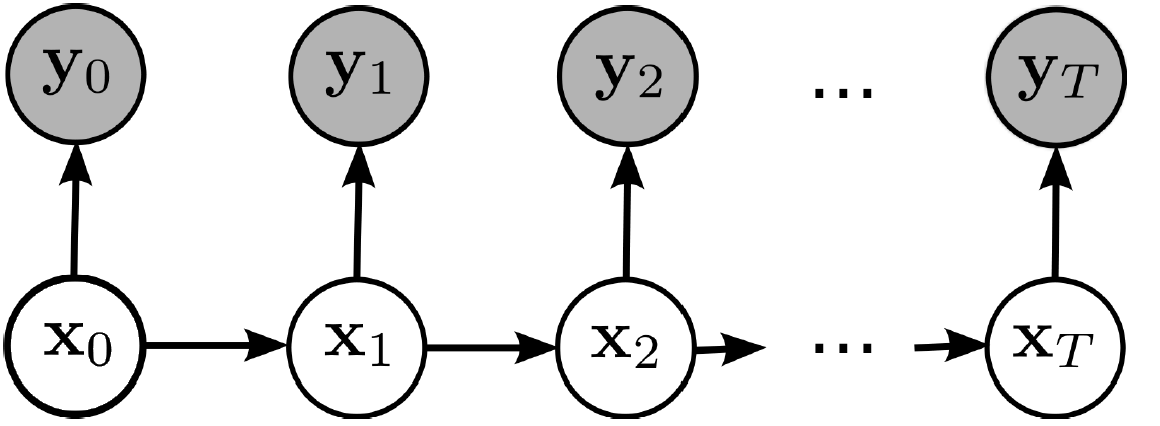
\includegraphics[width=0.7\textwidth]{hmm.png} 
\caption{Hidden Markov Models}
\label{fig:HMM}
\end{figure}

This class of models are designed to model evolving systems that output some observable events over time, which depends on the internal state of the system in a on-line manner. This imposes an implicit requirement on computation perspective: the estimate calculation cost should remain constant over time, i.e., the calculation cost does not increase with the increasing number of states.

Arguably, the most common inference problem in HMMs is the smoothing distribution, $p(x_{0:t} \mid y_{0:t})$, that is estimating the states $x_{0:t}$ based on the sequence of observations up to time $t$, $y_{0:t}$. Using Bayes rules, we can write the density of the distribution of interest in the recursion form as follows:
\begin{align}
    p(x_{0:t} \mid y_{0:t}) &= \dfrac{p(x_{0:t}, y_{0:t})}{p(y_{0:t})} \nonumber \\
                            &= \dfrac{p(x_{0:t-1}, y_{0:t-1})f(x_t \mid x_{t-1}) g(y_t \mid x_t)}{p(y_{0:t})} \nonumber \\ 
                            &= p(x_{0:t-1} \mid y_{0:t-1})\dfrac{f(x_t \mid x_{t-1}) g(y_t \mid x_t)}{p(y_t \mid y_{0:t-1})} 
\end{align}
This recursion is often re-written into two separate steps: the prediction step (the estimation of distribution of all states up to time $t$ given only states up to time $t-1$) and the update step (the correction of the predicted distribution taking into account the new observation) as follows:
\begin{align}
  p(x_{0:t} \mid y_{0:t-1}) &= p(x_{0:t-1} \mid y_{0:t-1})f(x_t \mid x_{t-1}) \nonumber \\
  p(x_{0:t} \mid y_{0:t})   &= \dfrac{p(x_{0:t} \mid y_{0:t-1}) g(y_t \mid x_t)}{p(y_t\
 \mid y_{0:t-1})}
\end{align}

Moreover, any smoothing distribution $p(x_{j:k} \mid y_{1:t})$ where $(0 \leq j \leq k\leq t)$ can be obtained by integrating out $x_i$ that are not interested in as follows:
\begin{equation}
  p(x_{j:k} \mid y_{0:t}) = \int p(x_{0:t} \mid y_{0:t}) dx_{0:j-1, k+1:t}
\label{eq:smoothing}
\end{equation}
A common smoothing distribution of interest is the marginal distribution at time $t$, $p(x_t \mid y_{0:t})$, which is also referred to as the filtering distribution.

Another distribution of interest is  the prediction distribution, that is the estimation of the distribution of any unseen \emph{future} states using only all observations up to current time. If we let $j = 0$ and $k \geq t$ in \eqref{eq:smoothing}, we obtain the following equation:
\begin{equation}
  p(x_{0:k} \mid y_{0:t}) = p(x_{0:t} \mid y_{0:t}) \prod^k_{i=t+1} f(x_i \mid x_{i-1})
\end{equation}
Therefore, any prediction density can be obtained by simply integrating out the variables of not interest from the above equation.

While these expressions \emph{appear} to be very simple, the distribution estimation problem is in fact far from being resolved in practice. The integrals involved in the above equations are often intractable because they require the evalution of complex high-dimensional integrals\footnote{Except under very special setting, in which the marginal filtering density $p(x_t \mid y_{0:t})$, the prediction density $p(x_t \mid y_{0:t-1})$ and the recursive likelihood $P(y_t \mid y_{0:t-1})$ are all Gaussian densities, then their means and variances can be computed analytically using Kalman Filter as shown in Appendix \ref{sec:KF}.}. 

\subsection{Sequential Important Sampling (SIS)}
\label{sec:SIS}
Sequential Monte Carlo provides a systematic way to approximate the solution to the distribution estimation problem. Let assume that it is possible to decompose the selected proposal distribution into recursion form as follows:
\begin{align}
	q_{0:t}(x_{0:t} \mid y_{0:t}) &= q_{0:t-1}(x_{0:t-1} \mid y_{0:t-1}) q_t(x_t \mid x_{0:t-1}, y_{0:t}) \nonumber \\
	             &= q_0(x_0 \mid y_0) \prod^t_{i=1} q_i(x_i \mid x_{0:i-1}, y_{0:i})
\label{eq:q}
\end{align}
then it is possible to obtain sample ${x_{0:t}}$ by first sampling $x_0 \sim q_0(\cdot)$ at time $0$ and then $x_i \sim q_i(x_i \mid x_{0:i-1}, y_{0:i})$ for all time $i$ from $1$ to $t$. The corresponding weight associated to each sample $x_{0:t}$ can also be decomposed into recursion form as follows:
\begin{align}
  \tilde{w_t} &= \dfrac{p_{0:t}(x_{0:t} \mid y_{0:t})}{q_{0:t}(x_{0:t} \mid y_{0:t})} \nonumber \\
%              &= \dfrac{p_{0:t-1}(x_{0:t-1} \mid y_{0:t-1})}{q_{0:t-1}(x_{0:t-1} \mid y_{0:t-1})} \dfrac{p_{0:t}(x_{0:t} \mid y_{0:t})}{p_{0:t-1}(x_{0:t-1} \mid y_{0:t-1})q_t(x_t \mid x_{0:t-1}, y_{0:t})} \nonumber \\
%              &= \tilde{w}_{t-1} \dfrac{p_{0:t}(x_{0:t} \mid y_{0:t})}{p_{0:t-1}(x_{0:t-1} \mid y_{0:t-1})q_t(x_t \mid x_{0:t-1}, y_{0:t})} \nonumber \\
              &\propto \tilde{w}_{t-1} \dfrac{f_t(x_t \mid x_{t-1})g_t(y_y \mid x_t)}{q_t(x_t \mid x_{0:t-1}, y_{0:t})} \label{eq:w} \\
              &\propto \tilde{w}_0 \prod^t_{i=1} \alpha_i(x_{i})          
%  &= w_0(x_0) \prod^t_{i=1} \frac{p_i(x_{0:i})}{p_{i-1}(x_{0:i-1})q_t(x_i \mid x_{0:i-1})} \nonumber \\
\end{align}
where $\alpha_t(x_{t})$  is often referred to as incremental importance weight function. This is the key concept in SIS.

Using these weighted samples $\{(x^{(i)}_{0:t}, \tilde{w}^{(i)}_t)\}_{1 \leq i \leq N}$, it is possible to estimate any function $f$ defined on the space using the self normalised importance sampling estimator in the same way as \eqref{eq:is} as follows:
\begin{align}
  \hat{f}(x_{0:t}) &= \sum^N_{i=1} \dfrac{\tilde{w}^{(i)}_t}{\sum^N_{j=1}\tilde{w}^{(j)}_t} f(x^{(i)}_{0:t}) \nonumber \\
   &= \sum^N_{i=1} \hat{w}^{(i)} f(x^{(i)}_{0:t})
\end{align}
A particular important instance of SMC is obtained when the prior distribution is used as the importance distribution:
\begin{align}
	q_{0:t}(x_{0:t} \mid y_{0:t}) &= p(x_{0:t}) \nonumber \\
	             &= p_0(x_0) \prod^t_{i=1} p_i(x_i \mid x_{0:i-1})
\label{eq:bf}
\end{align}
This greatly simplifies importance weight to follows:
\begin{equation}
  \tilde{w_t} \propto \tilde{w}_{t-1} g (y_t \mid x_{t}) 
\end{equation}
The SIS algorithm is summarised in Algorithm \ref{algo:sis}.

\begin{algorithm}
\caption{Sequential Importance Sampling}\label{algo:sis}
\begin{algorithmic}[1]
\Function{SequentialImportanceSampling}{N, T}
\State Set $t \gets 0$.
\State For $i \in 1, \ldots, N$, sample $x^{(i)}_0 \sim q(x^{(i)}_0 \mid y^{(i)}_0)$.
\State For $i \in 1, \ldots, N$, calculate the unnormalized importance weights:
\begin{equation*}
 \tilde{w}^{(i)}_0 = \dfrac{f(x_0^{(i)})g_0(y_0 \mid x^{(i)}_0)}{q_0(x^{(i)}_0 \mid y_0)}
\end{equation*}
\State For $i \in 1, \ldots, N$, normalize the importance weights:
\begin{equation*}
\hat{w}^{(i)}_0 = \dfrac{\tilde{w}^{(i)}_0}{\sum^N_{i=1} \tilde{w}^{(i)}_0}
\end{equation*}
\State Set $t \gets t + 1$.
\While{$t \leq T$}
\State For $i \in 1, \ldots, N$, sample $x^{(i)}_t \sim q(x^{(i)}_t \mid y_{t-1}, x^{(i)}_{t-1})$.
\State For $i \in 1, \ldots, N$, set $x^{(i)}_{0:t} \gets (x^{(i)}_{0:t-1}, x^{(i)}_t)$.
\State For $i \in 1, \ldots, N$, calculate the unnormalized importance weights:
\begin{equation*}
 \tilde{w}^{(i)}_t = w^{(i)}_{t-1} \dfrac{f_t(x^{(i)}_t \mid x^{(i)}_{t-1})g_t(y_t \mid x^{(i)}_t)}{q_t(x^{(i)}_t \mid x^{(i)}_{0:t-1}, y_{0:t})}
\end{equation*}
\State For $i \in 1, \ldots, N$, normalize the importance weights:
\begin{equation*}
\hat{w}^{(i)}_t = \dfrac{\tilde{w}^{(i)}_t}{\sum^N_{i=1} \tilde{w}^{(i)}_t}
\end{equation*}
\EndWhile
\EndFunction
\end{algorithmic}
\end{algorithm}

\subsection{Optimal Proposal Distribution}
While SIS is attractive, it is nothing but a specialised version of importance sampling introduced earlier in Section \ref{sec:IS}. As the state space increases with the number of time step $t$, direct importance sampling on a state space that is increasing in size is not very efficient. The weights of the samples will degenerate over time, in the sense that the weights start to concentrate only on a small number of samples. Consequently, many samples will have negligible weights and do not contribute much in the estimating the expectation. See \cite{JAM10} for a step-by-step illustration. The weight degeneracy issue cause the quality of the estimate degrades over time.

To alleviate this issue, looking at \eqref{eq:w}, it is obvious that the variance of importance weights can be minimised by using a proposal distribution of the following form:
\begin{equation}
 p_{t}(x_{t} \mid x_{t-1}, y_t) \propto f_{t}(x_{t} \mid x_{t-1}) g_{t}(y_{t} \mid x_t)
\end{equation}
This is often referred to as the optimal proposal distribution.

In general, it is not always possible to sample from this optimal proposal distribution. Yet, the knowledge of its form can be helpful in designing a reasonable good proposal distribution, which one can sample from. Better
proposal \emph{reduces} the amount of variance introduced, but it \emph{does not eliminate} the weight degeneracy problem.

\subsection{Sequential Importance Resampling (SIR)}
The variance in importance weights accumulates over iterations. This suggests a possible solution is to ``reset'' the weights associated to the samples somehow during the iterations \cite{JAM10}. Sequential Importance Resampling (SIR) introduces an additional resampling step to SIS step in a similar fashion as discussed in Section \ref{sec:IS}. After resampling, the weight of each sample is reset to be equal, i.e., $\frac{1}{N}$. This resampling step however introduces extra variance to the estimators.

A simple direct implementation of resampling step is to select the sample from the intermediate stage according to a Multinomial distribution with the success probability parameter set to the vector of normalised weights, $\hat{w}(x^{(i)})$, i.e., the chance of a sample point being replicated is proportional to its weight. 

There are many other resampling schemes have been proposed in the literature. For example, stratified resampling \cite{KG96} as the name suggested splitting the samples into strata to ensure the good coverage on the resulting sample set, residual resampling \cite{JSL98} which is able to decrease the variance of the weights due to resampling, etc. See \cite{DR05} for further details on the comparison of these sampling schemes.  The SIR algorithm is now summarised in Algorithm \ref{algo:sir}.

\subsection{Effective sample size (ESS)}
\label{sec:ess}
Resampling step induces additional Monte Carlo variance to the weights. Yet, this step is necessary to avoid accumulation of estimation variance onto the weights over time and therefore results in a more accurate estimate.

To trade-off these two competing requirements, one possible way is to monitor the effective sample size (ESS) of the sample set which provides a measure on the quality of the weighted samples. The ESS value can be estimated as follows:
\begin{equation}
  \text{ESS} \approx \dfrac{1}{E[w^2]} \approx \dfrac{\left(\sum^N_{i=0} w_i \right)^2}{\sum^N_{i=0}w_i^2}
\end{equation}

A common way to integrate this idea is to trigger the resampling step only if the ESS value at time step $t$ fall below certain threshold at time $t$, say $\frac{N}{2}$. See \cite{JAM10} for further details on ESS.

\begin{algorithm}
\caption{Sequential Importance Resampling}\label{algo:sir}
\begin{algorithmic}[1]
\Function{SequentialImportanceResampling}{N, T}
\State Use Steps $2$-$11$ of Algorithm \ref{algo:sis}
\State \textbf{Resample:} For $i \in 1, \ldots, N$, resample $ x^{(i)}_{0:t} \sim \dfrac{\sum^N_{i=1}\hat{w}^{(i)}_t\delta_{x^{(i)}_{0:t}}}{\sum^N_{j=1} \hat{w}^{(j)}_t}$
\EndFunction
\end{algorithmic}
\end{algorithm}

\subsection{Resample-Move Algorithm}
\label{sec:rm}
However, resampling is not a silver bullet for sampling impoverishment. Essentially, resampling provides a mechanism to eliminate low weight samples to give way to replicate \emph{copies} of high weight samples. This allows all samples to participate and contribute to the distribution estimation. This is obvious beneficial for the case of estimating filtering distribution and predictive distribution. Over time, this replication results in decrease in the number of distinct samples for previous time steps. Eventually, many samples will have the share the same sample trajectory. This is a fundamental weakness of SMC, in which the sample path history is never re-written. This lose of diversity in the sample set will have a negative impact when it comes to any smoothing distribution estimation. 

To counteract this sample impoverishment, Resample-Move Algorithm \cite{BC01, WG01} is proposed to introduce some perturbation to the samples (so to diversify them) without changing the distribution they represent. In the original paper, this is accomplished by adding a MCMC ``move'' step to each sample after the resampling step with a Markov Kernel, $K$ that is invariant to the target distribution, $p(\cdot)$. This Resample-Move algorithm is summarised in Algorithm \ref{algo:rm}.

This does not entirely solve the smoothing distribution estimation problem. To apply Markov Kernels with invariant distribution corresponding to the smoothing distribution, the space that Markov kernel is defined has to increase at each iteration. This implies the computation time increases linearly with time. Moreover, fast mixing high dimension Markov kernel in itself is not easy to design \cite{JAM10}.

To trade-off between the two requirements, one could adopt a sliding windows approach, in which the MCMC Kernel is used to diversify only the samples of the previous $n$ time step at each iteration. Adding this sliding window approach into the standard SIR algorithm will make each iteration has an additional \emph{fixed} computational cost.

\begin{algorithm}
\caption{Resample-Move Algorithm}\label{algo:rm}
\begin{algorithmic}[1]
\Function{ResampleMoveAlgorithm}{N, T}
\State Use Steps $2$-$11$ of Algorithm \ref{algo:sis}
\State \textbf{Resample:} For $i \in 1, \ldots, N$, resample $ x^{(i)}_{0:t} \sim \dfrac{\sum^N_{i=1}\hat{w}^{(i)}_t\delta_{x^{(i)}_{0:t}}}{\sum^N_{j=1} \hat{w}^{(j)}_t}$
\State \textbf{Move:} For $i \in 1, \ldots, N$, sample $x^{(i)}_{0:t} \sim K_t(\cdot)$, where $K_t$ is $p_t$-invariant.
\EndFunction
\end{algorithmic}
\end{algorithm}

\subsection{Rao-Blackwellised SMC}
\label{sec:msmc}
In practice, many models may not be entirely non-linear or non-Gaussian. Some states may be linear and Gaussian, conditional upon other states. Instead of naively modelling all state spaces using SMC, a better approach would be carrying out analytical computation as possible on the linear Gaussian states and use SMC model only the non-linear states. This marginalisation setting will yield estimate that has smaller variance.

To illustrate this, let consider the a simple conditional linear Gaussian Model as follows:
\begin{align}
  X^L_t &= A_t(X^N_t)X^L_{t-1} + B_t(X^N_t)W_t + F_t(X^N_t) \\
  Y_t &= C_t(X^N_t)X^L_t + D_t(X^N_t)V_t + G_t(X^N_t)
\end{align}
where $\{X^N_t\}_{t \geq 0}$ is a non-linear Markov processs, $A_t$, $B_t$, $C_t$, $D_t$, $F_t$, $G_t$ are appropriate matrix/vector of $X^N_t$ and  $\{W_t\}_{t \geq 0}$ and  $\{V_t\}_{t \geq 0}$ are independent sequences of standard Gaussian random variable, i.e., $W_t, V_t \sim \mathcal{N}(0,I)$. In such a case, the transition density and likelihood of this model are Gaussian distributions with center lied at a point of a linear combination of the known $x^N_t$ that can be obtained by using classical Kalman Fitering recursions as shown in Appendix \ref{sec:KF}.


The discussion here has been focused on conditional linear Gaussian model. The discrete state space HMMs is another important class of HMMs in which HMM forward algorithm \cite{LRR89} can be used to marginalise the internal states. See \cite{CO05} for further details.


\section{Conclusion}
This chapter presents a review of Monte Carlo methods, with a particular focus on Sequential Monte Carlo (SMC), along with various extensions proposed in the literature, used in this thesis for portfolio optimisation.

It is worth to have a remark here that the SMC are not only applicable to sequential filtering problem. For example, it has been established that it is possible to use SMC within MCMC framework (pMCMC, where p stands for particle) \cite{CA10} to build high dimensional proposal distribution to improve standard MCMC. In the next chapter, we will show how SMC can be used as a maximiser to search for a optimal strategy for the optimal portfolio, given a multiplicative reward function.

% ------------------------------------------------------------------------


%%% Local Variables: 
%%% mode: latex
%%% TeX-master: "../thesis"
%%% End: 

%\chapter{Security Policy Models}
\graphicspath{{Chapter3/figures/}}
\label{SecurityPolicyModels}
A security policy is
\begin{quote}
  a set of rules~(or principles) that direct how a system~(or an
  organisation) provides security services to protect sensitive and
  critical system resources~\cite{RS07}.
\end{quote}
A security policy must therefore specify \emph{all} necessary control
measures for ensuring system security, including how authentication
should be done and what responses should be made to a security
violation, etc.

Access control specification is typically a major component of a
security policy. Access control protects the resources of a
system~(objects) against unauthorised access by restricting the use of
system resources only to the authorised users~(subjects) according to
the security policy of the system~\cite{RS07}. Access can be in many
modes; the common ones include read, write, append and execute. The
access mode that a subject has on the objects in the system is known
as the~``privilege'' the subject has. The set of high-level rules that
specifies which accesses are to be authorised and which are not is
known as the access control policy~\cite{PS01}. The study of access
control policies has resulted in various useful models. Most of these
models are formal, i.e., formal analysis can be carried out to prove
the models are secure with respect to the security objectives
concerned. There are also some models consisting of informal
high-level principles such as the Clark-Wilson model~\cite{DDC87}.

This chapter first reviews the traditionally influential security
policies and models in the literature. It then presents some recently
proposed risk-budget based models that aim to provide more
flexibility. Next, it introduces the top-down policy hierarchical
model that enables policy composition and refinement, with an emphasis
on the problems encountered in the refinement and conflict analysis
processes. Lastly, it summarises the current state of the art in
security policy development and reiterates the research objectives of
the thesis.

\subsection{Economics based models}
\label{JASONEconomicsBasedModel}
The idea of managing risk in access control using economic concepts is
proposed in~\cite{JPO04}. Each user in an organisation is allocated a
number of risk tokens, which can be spent for operational needs. The
number of risk tokens a user will get in the future depends on the
return of investment of the user. Essentially, risk is viewed as a
type of limited resource in an organisation and the access control
problem is transformed into a resource allocation problem. Two
economics based models are introduced: one based on the command
economic system and the other based on the market economic system.

% The proposal is done in three incremental phases. The first phase is
% the preparatory phase, where the necessary components in making the
% system work are discussed. The following two phases introduce two
% models: the command economy system~(also known as the push economy
% system) and the market economy system~(also known as the pull economy
% system).

\subsubsection{Definition of risk, damage and harm}
\label{sec:ebsdefinitionofriskharmanddamage}
New definitions for risk and two new terms,~``damage'' and~``harm''
are introduced in~\cite{JPO04}. Risk is defined as the unnormalised
probability of an access which can cause the loss of a secret, damage
is defined as the cost of the loss, and harm is defined as the
expected cost of the loss. These terms are related as follows:
\begin{equation}
  \text{harm} = \text{damage} \times \text{risk} 
\label{eq:ebsharm}
\end{equation}
The definition of risk is different from the one in the Fuzzy MLS
model~\eqref{eq:risk}, which is restated as follows for ease of
reference:
\begin{equation*}
  \text{risk} = (\text{value of damage, }V) \times (\text{probability of incurring the damage, }P) 
\end{equation*}

A careful examination of both equations allows us to establish a
mapping between the terms: the term~``harm'' here corresponds to the
term~``risk'' in the Fuzzy MLS model; the term~``damage'' holds the
same meaning in both cases; and the term~``risk'' here corresponds to
the term~``probability of incurring a damage'' in the Fuzzy MLS
model. In this thesis, the terms are used in the sense of the original
report for ease of reference.

\subsubsection{Three guiding principles}
\label{sec:ebsprinciples}
The author suggests that the new information protection systems should
be risk based and outlines three principles that should be followed in
building them. These principles are as follows:
\begin{enumerate}
\item Measure risk --- The amount of risk associated with each
  access should be measured or at least estimated.
\item Mark an acceptable risk level --- Risk avoidance~(setting the
  acceptable risk level to zero) effectively stops all the information
  accesses because every access has an inherent amount of risk
  associated with it. The acceptable risk level should be set to a
  value that optimises the long-term benefit.
\item Maximise the information flow up to the acceptable level --- In
  contrast to current systems which attempt to minimise the total
  risk, information in the system should flow to the greatest extent
  compatible with the acceptable risk level in order to optimise gain.
\end{enumerate}

\subsubsection{Risk model}
\label{sec:ebsriskmodel}
A risk model is required to estimate the risk of each access. The
following factors should be considered in building this model:
\begin{description}
\item [Individual factors] --- User roles, security clearances,
  previous positions, etc.
\item [Situational factors] --- Operational environment,
  access time, etc.
\item [Technical factors] --- Hardware/software security measures,
  etc.
\item [Types of accesses] --- Access method~(softcopy vs.\ hardcopy),
  access duration, whether access is auditable, whether information
  can be redistributed, etc.
\item [Temporal effects of consequences] --- Leaking the information
  on the budget allocated for a small project may result in a
  short-term risk but leaking the information on a national secret
  weapon may result in a long-term risk.
\end{description}
These factors have to be combined in a mathematical way to yield a
formula that can be used to assign a risk value to each information
access.

\subsubsection{Model based on command economic system}
\label{sec:ebscommandeconomysystem}
In this model, the value of a token is pegged to
risk~\cite{JPO04}. For example,
\begin{quote}
  $1$ token is pegged to the risk associated with softcopy access for
  a day to a document by an individual who is cleared to the secret
  level.
\label{def:ebstoken}
\end{quote}
The value of the token is associated with the estimated risk incurred
in the access, including the type and duration of the access and the
security clearance of the individual. Yet, it does not consider the
value of the document~(the damage factor).

Using the risk model presented in Section~\ref{sec:ebsriskmodel}, each
access can be associated with a certain number of risk tokens. Higher
risk accesses cost more. For example,
\begin{itemize}
\item Softcopy access for a day to a document by an individual who is
  cleared to top secret level costs~$0.2$ token.
\item Hardcopy access to a document with a restriction on further
  distribution by an individual who is cleared to secret level
  costs~$50$ tokens.
\end{itemize}
When a piece of information is being produced, the producer will
create the number of tokens that is commensurate with the acceptable
risk level of the piece of information. For example, the production of
a document that may be viewed in softcopy for~$500$ times by an
individual who is cleared to secret level is always accompanied by the
creation of~$500$ tokens. If the~$500$ tokens are spent by an
individual who is cleared to secret level to print the document in
hardcopy format for $10$ times with a restriction of no further
distribution, the acceptable risk level of the document would still be
considered reached.

Additionally, the use of different types of tokens is necessary for
different types of information. This is because all tokens are pegged
using the same baseline. More sensitive information has less tolerable
risk level and therefore has fewer tokens created with it.

To increase the liquidity of the market, a secondary market can be
introduced to allow token exchange. This does not require any change
of the model because the tolerable risk of the information has been
controlled by the number of tokens created with it and other risk
factors have been taken care of in the cost associated to each
information access.

To distribute the risk tokens, the information producers create and
distribute the risk tokens to different organisations based on their
needs. Within an organisation, risk tokens are pushed down through the
management hierarchy. Periodically, the distribution is reviewed based
on the return on investment function. Other metrics can also be used
to adjust the distribution of the risk tokens. An example of such
metric is the utilisation function that measures the fraction of
tokens that have been spent to purchase information accesses. This
function can also serve as a measure on the merits of the information
producers. If the utilisation fraction is near $100\%$, it means the
organisation is almost reaping the full benefit of the information
produced and vice versa.

\subsubsection{Model based on market economic system}
\label{sec:ebsmarketeconomysystem}
The main aspect that differentiates this model from the model based on
command economic system is the collapse of information specific tokens
into two general types. This removes the controls that the producers
have in setting the tolerable risk associated with the
information~(via manipulation of the number of tokens created). The
reason for having more than one type of token is that different types
of information require different protection profiles over time. This
change requires the value of a risk token and the token distribution
mechanism to be redefined.

In the model based on command economic system, accessing to any
information, regardless of its sensitivity level, would cost the same
number of token for all individuals with the same clearance
level. This is because the risk of an information access is only
associated with the probability of causing unauthorised disclosure of
the information. However, the amount of damages caused by unauthorised
disclosure of information with different sensitivity levels are likely
to be different. More sensitive information are likely to cause more
damage. To control the amount of damage, the information producer can
limit the number of tokens created along with an information. With the
change from information-specific tokens to generic tokens, this is no
longer possible.

To overcome this problem, the value of a token in this new model is
changed to be associated with harm~($\text{damage} \times
\text{risk}$) as defined in~\eqref{eq:ebsharm}. To calculate harm, an
additional damage model is required. For risk token creation and
distribution, a new central authority that plays a similar role to the
central bank in the real world is introduced. This central authority
is also responsible for monitoring the health of the tokens by
balancing demand and supply, and controlling the inflation and
deflation rates.

\subsubsection{Review}
\label{sec:ebsreview}
Although the author advocates that the model based on the market economic
system as being better than the model based on the command economic
system, we think that there are interesting features and tradeoffs in
both models. As shown in Table~\ref{tbl:EBSComparison}, the value of a
token is defined in different ways. The model based on the command
economic system has been deliberately simplified to introduce the new
concept and to make way for the model based on the market economic
system. This advocation may also be compounded by an implicit
assumption that the market economy is better than the command economy
in the real world.
\begin{table}
\centering
\begin{tabular}{|p{0.2\textwidth}|p{0.35\textwidth}|p{0.35\textwidth}|}
  \hline
                   & Command economic system   & Market economics system\\
  \hline
  Token value      & pegged with risk          & pegged with harm\\
  \hline
  Token type       & information-specific      & two generic types: short-term and long-term\\
  \hline
  Token creator    & information producer      & central authority~(central bank)\\
  \hline
  Model required   & a risk model only         & a risk model and a damage model\\
  \hline
  Information risk & managed by limiting the number of tokens created with information & managed by maintaining the equilibrium of the information market\\
  \hline
\end{tabular}
\caption{The differences between the model based on command economic system and the model based on market economic system.}
\label{tbl:EBSComparison}
\end{table}

To have a fair comparison, the value of a token in the model based on
the command economic system is associated with the amount of
damage. The only remaining difference now is the controls the
producers have in setting the tolerable damage associated with
information in the model based on the command economic system. The
information producers can be dishonest in their claims of the
sensitivity levels of information by manipulating the number of tokens
created with them. This may result in market dislocation. The model
based on the market economic system is proposed to alleviate this
problem by the introduction of a central bank, thus making the
credibility of the central bank a key factor for this new model to
operate properly. In other words, the author assumes that the risk of
the central bank in being compromised is smaller than the risk of
market dislocation caused by the dishonest behaviours of the
information producers. This assumption may not hold true in certain
operational environments, e.g., MANETs do not have a central trusted
node and all nodes are exposed to security attacks.

Having said that, the three guiding principles in building a
protection system as outlined in Section~\ref{sec:ebsprinciples} are
inspiring. Current protection systems always attempt to minimise the
risk incurred in each access in the hope that the total risk of all
accesses is below the acceptable risk threshold limit. These
principles recognise that risk is inevitably incurred in each access
and thus advocate managing the global risk. The acceptable risk
threshold limit is first determined and information flow is encouraged
all the way up to the acceptable limit to maximise the gain. This
provides greater short-term flexibility in the access
control. Information is made available to any user who is willing to
pay the cost, yet the long-term behaviours of users remain under
control as the token distribution is subject to the return on
investment of each user.

The distribution of risk tokens based on the return on investment also
encourages each user to opt to access information in safer ways so as
to reduce expenses. A stricter enforcement on using safer access
methods can be achieved by reducing the number of tokens given to the
individual. If the tokens are spent in the usage of a
riskier~(expensive) way to access information, the individual may not
have sufficient tokens to accomplish other duties assigned.

There is a natural reluctance for human users to make decisions that
have far reaching consequences, e.g., revoking the clearance of a
user. The risk model helps by redefining the responsibilities of a
human user in terms of security and operational duties. The security
duty encompasses ensuring the integrity of the information entered to
the risk model. This incremental information input to the risk model,
which gradually changes the trust levels of a user, becomes less
daunting in comparison to the immediate revocation of the clearance of
a user. The operational duty is to ensure that the tokens are used or
distributed wisely in the organisation/team, e.g., a manager may make
an economic decision in distributing the tasks to his employees.
However, the use of the risk model leads to an accountability issue:
who is going to be responsible when something goes wrong? The risk
model, the user or the higher level organisation?  There is no obvious
answer. Without accountability, the number of misuses is likely to
increase.

In economics based models, the availability of information access is
tightly linked to the risk tokens. A user who has spent all his budget
is rendered useless until the next token distribution cycle. This can
happen due to the use of an imperfect risk model, an imbalanced
distribution of risk tokens or misbehaviours of users. In the former
two cases, continual refinements have to be employed in a timely
manner to avoid causing market dislocation. If it is due to the
misbehaviours of users, simply denying the user's access request can
be a logical answer but inappropriate in certain scenarios. For
example, denying an information access to a front-line commander in a
battlefield who has no budget left may result in fatal casualty.

Both models also assume that entities are rational and therefore will
make the best decision among given choices. However, psychological and
social research suggests otherwise; the human decision-making process
is often suboptimal and irrational. For example, the~``heuristics and
biases'' programme was started to investigate the idea of whether the
decision-making process under uncertainty often rests on a limited
number of simplified heuristics\footnote{Heuristics are the simple yet
  efficient informal rules that humans use to make decisions.} or a
complicated algorithm~\cite{AT74}. One of the results was the framing
effect, which showed that the way a problem is formulated can have
influence on the decision-making process~\cite{AT81}. A problem can
emphasize on a gain~($30\%$ of the people will pass the examination)
or on loss~($70\%$ of the people will fail the examination). The
former case generally leads to risk aversion behaviour while the
latter case generally leads to risk seeking behaviour. Relationship
among people can also have effects on the decision-making process. For
example, a captain may choose not to report the misuse of authority
among his soldiers to protect his soldiers from punishment or to
preserve the reputation of his team. Other factors such as emotion,
bias, mistake or incapability in judgement~\cite{DK82} can also creep
into the decision-making process and cause chaos in the system.

Whilst the general view of the system architecture and factors to be
considered are outlined in~\cite{JPO04}, it does not present any
example of core components, e.g., the models to calculate risk and
damage. These models are inherently complicated to design and
build. The contributing factors are difficult to measure, quantify,
calculate and aggregate, e.g., how secure is an operating system?
Should an access to a secret document be considered a short-term risk,
a long-term risk or both? If both, what is the proportion of each
risk? Even if building such models is possible, the task of fine
tuning these models in a timely manner can be
challenging. Furthermore, other security prerequisites on the
infrastructures required to implement the system, as discussed
in~\cite{JPO04}, ranging from network protocol to technologies on
tamper proof hardware, are difficult to have. The security of a system
is only as strong as its weakest component; breaching just one
requirement can easily lead to a security breach of the system.

%\subsubsection{Summary}
%\label{JASONEconomybasedModel.Summary}
In summary, the use of economic concepts may provide greater
flexibility to protect information systems. However, there are doubts
arising from its implementation and also with regard to some practical
issues of the system. Indeed, the author also commented that~``(they)
fully expect that much of what~(they) suggest can be proved
unworkable, or no better than some different approach'' and~``(this)
model may seem too extreme''~\cite{JPO04}. Further research is
required to further investigate this idea. Having said that, the $3$M
principles of building an information protection system: measure risk,
mark the acceptable risk and maximise the information distribution to
the acceptable level are inspiring thoughts.

\subsection{Top-down hierarchical models}
\label{TopDownHierarchicalPolicyModel}
The models presented so far have access control policies which are
specified in terms of the low-level corresponding enforcement
mechanisms, e.g., protection bits, capabilities and access control
lists. Each model implements a single specified policy but does not
often capture all the protection requirements of a system.

\subsubsection{The requirements of the policy languages}
In~\cite{TYCW92}, Woo et al.\ proposed a logic based language that
allows access control policies to be specified independently from the
implementation mechanisms and two composition operators that can be
used to combine multiple access control policies. They also outlined a
list of requirements for a language to be suitable for specifying
access control policy. The language should:
\begin{enumerate}
\item be declarative and semantically independent from the
  implementation mechanisms.
\item be efficiently computable, hence allowing efficient
  authorisation evaluation.
\item allow the intended security properties to be easily specified.
\item allow the ways to handle authorisation be easily specified when
  policies are non-monotonic, inconsistent, incomplete~(coverage) or
  combined together.
\end{enumerate}

Although it has been found later in~\cite{SJ01} that the language
proposed does not impose sufficient constraints to ensure that the
specified policy is Turing decidable and therefore may not be
implementable, their work has pioneered the use of high-level
languages to specify abstract policies independently from the
implementation mechanisms. In~\cite{SJ97,SJ97A}, the Authorisation
Specification Language~(ASL), which is based on stratified first order
logic, became the first complete and computable policy specification
language. Other policy specification languages also exist in the
literature, e.g., Security Policy Language~(SPL)~\cite{CNR01} and
XACML~\cite{SD03}. Refer to~\cite{MS02} for detail.

\subsubsection{Policy hierarchy}
In network management research, policies have become increasingly
popular as a means of managing distributed systems. Here the
term~``policies'' carries a much broader meaning; policies are~``rules
governing the choices in behaviour of a system~(in
general)''~\cite{MS94}. Therefore, policies encompass not only
security-related rules, but also management rules. For example,
obligation policies which have the form of event triggered
condition-action rules can be used to define adaptive management
actions, e.g., change in the quality of service provided, resource
allocation and backup policy and software installation. This
difference is not important in the discussion of this thesis.

To cope with the growth in size and complexity of large distributed
systems, there is a trend towards automating many aspects of
management into distributed components. The concepts of viewing policy
as an object and of policy hierarchy are first proposed
in~\cite{JDM91} and refined further in~\cite{JDM93,JDM93A}. The
concept of viewing a policy as an object is about decoupling the
policy from the components that are responsible for enforcing it~(the
implementation mechanisms) and viewing the policy as an independent
reusable component~\cite{JDM91}. This enables the behaviour of the
system to change by simply changing the rules in the policy.

The concept of policy hierarchy recognises that policies exist at
different levels of abstraction. It suggests that high-level policies
can be derived from business goals and form the basis of multiple
low-level policies~\cite{JDM91,JDM93}. The ultimate objective is to
develop a mechanism that allows the specification of a high-level
policy to be analysed and translated automatically to low-level
policies which can then be executed by the system. The number of
policy hierarchy levels may vary among different models, yet the
intuition remains the same. The high-level policies are refined to
form low-level policies.

As an example, the policy model proposed in the International
Technology Alliance~(ITA) project is shown in
Figure~\ref{fig:ITAPolicyModel}~\cite{KS08}. The model consists of
four layers: specification layer, abstract layer, concrete layer and
executable layer. The specification layer consists of authoring and
analysis tools that support the specification of high-level security
policies in constrained natural languages. These policies are then
refined into abstract policies. At the next layer, various formal
methods are used to check the correctness and consistency of these
abstract policies. The concrete layer is then responsible for refining
the analysed policies into concrete policies which are then upheld by
different components to meet the policy goals. The executable layer
transforms these concrete policies into executable policies and
distributes them to the implementation devices that are responsible
for enforcing the policies. This bottom layer is also responsible for
reporting the status and device discovery information back up to the
concrete policy layer.

\begin{figure}[htbp]
 \centering
 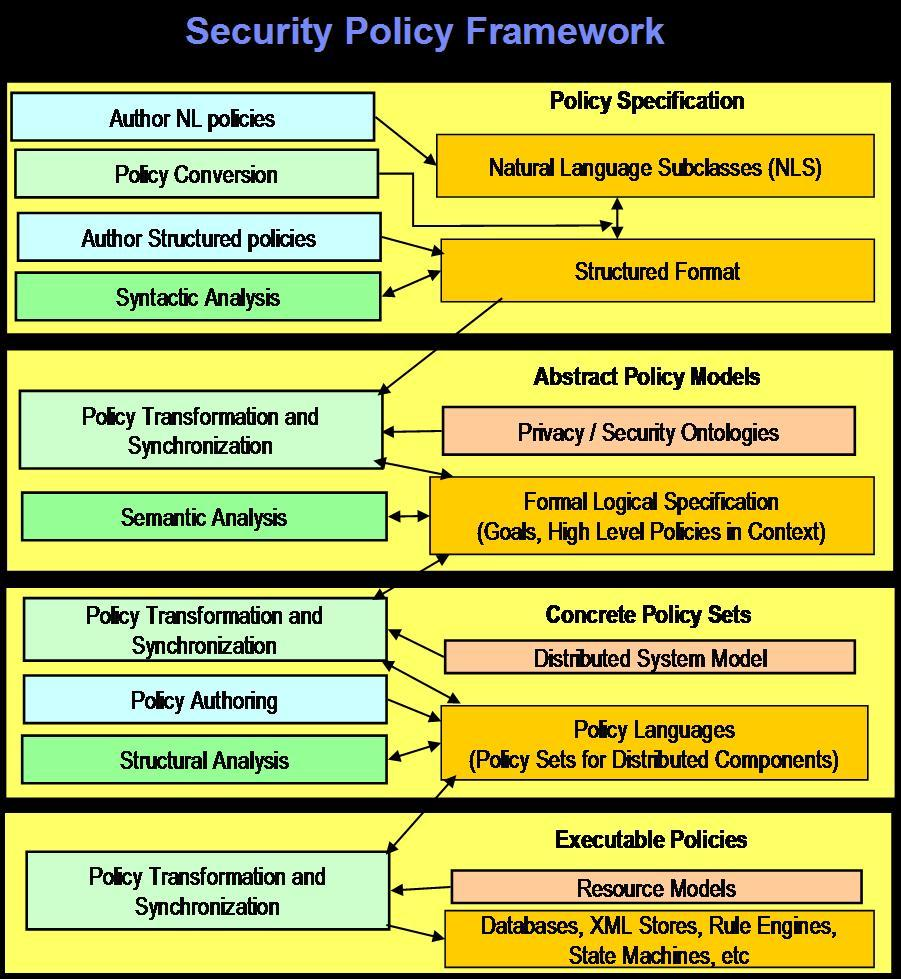
\includegraphics[width=\textwidth]{ITAPolicyModel}
 \caption{The ITA policy model~\cite{KS08}.}
 \label{fig:ITAPolicyModel}
\end{figure}
% In the following sections, we will discuss some of the issues in the
% processes in refining high-level policies into lower-level policies
% and analysing policies. 

\subsubsection{Policy refinement and policy conflict analysis}
\label{PolicyRefinementAndPolicyConflictAnalysis}
Policy refinement is the process of transforming high-level security
goals into low-level policies that can be enforced by a
system~\cite{JDM91}.  The refinement process involves the analysis of
policy conflict, policy coverage and the determination of resources
required to implement the policies~\cite{JDM91}.

One widely accepted policy refinement approach is the goal refinement
approach proposed in~\cite{RD97}. The goal refinement approach
consists of the process of identifying, recognising and instantiating
refinement patterns. Once a refinement pattern has been identified and
analysed for completeness and conflict, any policy that matches this
pattern is certain to be complete and correct. Whilst it is desirable
to have a fully automated refinement process, Moffett et al.\ argued
that it is often infeasible to do this in many situations other than
the most trivial scenarios~\cite{JDM93A}.

Policy conflict analysis is the process of verifying whether the
security policy is \emph{consistent} and
\emph{complete}~\cite{MS94}. By consistent we mean that there is no
conflict between the rules in the policies and with the capabilities
of the underlying system. By complete we mean the policy implements
all the high-level goals specified.

There are two categories of conflicts: modality conflicts and semantic
conflicts. Modality conflicts arise when the rules in the security
policies are inconsistent with one another. Modality conflicts can be
divided into the following three categories based on the types of
rules that are in conflict~\cite{EL99}:
\begin{enumerate}
\item Authorisation conflicts --- conflicts that arise because both
  positive and negative authorisation rules exist for the same action,
  subject and object tuple. In other words, a subject is
  authorised~(by the positive authorisation rule) as well as
  forbidden~(by the negative authorisation rule) to perform the same
  action on an object.
\item Obligation conflicts --- conflicts that arise because there is
  an obligation rule and a refrain~(negative obligation) rule defined
  for an action that a subject is obligated to perform as well as
  refrained from performing on an object.
\item Unauthorised obligation conflicts --- conflicts that arise
  when there are an obligation rule and a negative authorisation rule
  defined for an action that a subject is obligated but forbidden to
  perform on an object.
\end{enumerate}
Having a positive authorisation rule and a refrain rule defined for
the same action for a subject and an object is not considered as a
conflict.

Poor policy specification is not the only cause of policy
conflict. Organisation goals may be ambiguous and conflicting in
nature, e.g., maximising resource utilisation vs.\ maximising resource
availability. This will inevitably result in conflicts among policies
that are derived from it.
 
To detect these conflicts, syntactic analysis can be applied to the
policies to determine the overlap of subjects, targets and
actions~\cite{EL99}. However, the existence of overlap only reveals
the \emph{potential} modality conflict because other constraints, such
as time, might limit the applicability of the rules. Moreover,
syntactic analysis is unable to detect application-specific conflicts,
e.g., the separation of duty principle described in
Section~\ref{ClarkWilsonModel}. To detect these conflicts, the
conditions that may cause the conflicts are required to be specified
as additional constraints on the policies. The occurrence of the
conflicts may also depend on the state of the system. Analysing all
these states to check for possible conflicts is often infeasible and
therefore run-time analysis is still necessary.

Once these conflicts are detected, it is necessary to resolve
them. Jajodia et al.\ suggested a few ways to handle the conflicts
in~\cite{SJ97}. The simplest way is to do nothing but flag an error
condition. A better solution is to allow the positive authorisation
policy to override the negative authorisation policy or vice
versa. Often, the priority is given to the negative authorisation
policy based on the assumption that preventing actions would incur
less risk. Obviously this is not always true. For example, a positive
authorisation policy can be an exception to a more general negative
authorisation policy.

To alleviate this issue, priorities can be assigned to different
policies explicitly~\cite{EL99}. When conflicts arise among policies,
the highest priority policy is enforced. However, the task of priority
assignment in itself is difficult. There is also a problem of breaking
a tie if there are two or more policies with the same level of
priority. This problem is exacerbated when there are multiple parties
involved in defining and assigning policies. Inconsistency can easily
arise as each party can have different preferences. An alternative
approach is to define priority based on specificity of the
policy~\cite{AH90}. At the other extreme, meta policies are also being
proposed as a way to define the precedence relationship among
policies~\cite{EL99}. Whilst these resolution mechanisms provide more
flexibility, they also make the task of ensuring policy consistency
more complicated.  There is still no known general mechanism that is
able to detect and resolve conflicts among policies when arbitrary
conditions are allowed.

% As modern systems become more distributed, the distribution of the
% analysis procedures across the system can be problematic. The system
% can be organised in an unstructured order; each subsystem can be owned
% by different domains. This makes the policy refinement process much
% more complicated. In MANETs, subsystems can join, leave and rejoin at
% any time. This dynamic behaviour can easily cause conflicts among the
% policies.

%\subsubsection{Summary}
%\label{TopDownHierarchicalPolicyModel.Summary}
%This section presents a top-down hierarchical policy model in which
%policies are specified using high-level languages and then refined
%into low-level policies. Various issues related to the policy
%refinement process are discussed, including how conflicts among the
%policies can arise, be detected and be resolved.

\section{Summary}
\label{Review}
Recent research~\cite{JPO04} suggests that current static security
policy models are not appropriate for many modern systems, especially
when the operational environment is highly dynamic. Some models that
provide more flexibility have been
proposed~\cite{PCC07,PCC07A,JPO04}. These models are different from
the static ones in two important aspects. Firstly, the risk-benefit
tradeoff assessment on an information access request is no encoded in
the security policy itself. Instead, an explicit risk model is used in
these models to dynamically estimate the risk of an information access
request to make better informed decisions. Secondly, the new model
attempts to manage the total risk of a system as a whole, as opposed
to the risk of each access individually in the traditional
models. Users are allocated with an initial budget of risk tokens,
which they may use on their discretion to access different
information. The budget distribution is reviewed periodically based on
the benefit gained from information access of each user. However, the
models proposed are rather abstract. Many aspects of the models
require further investigation. These include the way to allocate
initial budget, the type of the market, the cost of the access, etc.

In the network management research, the top-down policy refinement
approach has received much attention recently. The idea of this
approach is to refine business goals to high-level security policies,
which in turn are refined into low-level policies
automatically. Whilst this conceptual idea is great, the current
policy conflict resolution mechanisms are still rather
primitive. There is currently no general mechanism that is able to
detect and resolve conflicts among policies when arbitrary conditions
are allowed. As modern systems become more distributed, the
distribution of the analysis procedures across the system can be
problematic. The system can be organised in an unstructured order;
each subsystem can be owned by different domains. This makes the
policy refinement process much more complicated.  In MANETs,
subsystems can join, leave and rejoin at any time. This dynamic
behaviour can easily cause conflicts among the policies.

The way we choose to approach the problem is a radical one. In this
thesis, we investigate how a specific set of decisions may be
generalised into an applicable security policy using EAs. A developed
policy inference system could be doubly useful. The generated policy
rules can be used on it own or used to verify the correctness of
existing policies. In a highly dynamic operational environment like
MANETs, where the risk factors are constantly changing, the inference
techniques must be able to dynamically update the policies inferred to
maintain their optimality. Here we explore the potential of EAs in
dynamically updating security policies with new decision
examples. Additionally, we observe that the risk-budget based policy
models reviewed in Section~\ref{FlexibleAccessControlModels} are
really families of policies. Each instance in a policy family
constrains the system and therefore affects the operational behaviour
and effectiveness of the system in its own way. We introduce the
notion of mission-specific policy and demonstrate how EAs can be used
to search for the~(near) optimal policies that fit a specific set of
missions using simulation runs~(instead of a set of decision
examples).

\section{Conclusions}
\label{SecurityPolicy.Conclusion}
This chapter summarises various influential security policies and
models in the literature. It then introduces the top-down hierarchical
policy model in which allows policies to be specified using high-level
languages and then refined into low-level policies. Various issues
related to the policy refinement and conflict analysis process are
discussed. Lastly, it reviews the current state of the art in security
policy development and reiterates the research objectives of the
thesis.


% ------------------------------------------------------------------------


%%% Local Variables: 
%%% mode: latex
%%% TeX-master: "../thesis"
%%% End: 

\chapter{Portfolio optimisation}
\graphicspath{{Chapter4/figures/}}
\label{cha:po}
Optimal portfolio is the ultimate goal of every investment manager; but the optimality criteria can be very different to each of them. In the infamous Markowitz's modern portfolio theory \cite{HM52}, it is assumed that investor attempt to maximise the return and minimise the risk of his portfolio. For index tracker fund manager, the main objective of portfolio management is to track and replicate the exposure of a benchmark index. The lack of active management generally makes the fund less vulnerable to change of management and has the advantages of lower fees and taxes. It is the latter the focus of the thesis lies.
 
In this chapter, we introduces the index tracking fund and summarise some causing factors of the tracking error between the fund and its benchmark index. We then present how the portfolio optimisation problem in terms of minimising the tracking error can be formulated as a stochastic control problem. Lastly, we show this stochastic control problem can be turned into a path-space parameter estimation problem, in which Rao-Blackwellised SMC can be used to estimate these parameters efficiently.
 
\section{Index tracking fund}
An financial index can be thought of a summary statistics of a market, typically formed as weighted average of the prices of some financial instruments. For example, FTSE 100 is an index that attempts to represents the performance of the 100 biggest companies in UK. This index is however not an investable financial product one can invest directly.
 
To allows investors to take exposure to the markets (as represented by the indices), index tracker funds are introduced. These funds generally follow very strict and transparent rules with the main objective to track their benchmark indices as close as possible. Investors of these funds therefore are only exposed to the market risks of the chosen indices, with minimal exposure to the risk associated with the investment process of the traditional active fund management.
 
\subsection{Index replication}
\label{sec:replication}
To track an index, the simplest way is to replicate the index by investing all the components of the benchmark index. However, this can be costly and difficult to manage, considering some of the indices may have huge number of components, e.g., MSCI World index that consists of $\approx 1600$ components from many different countries. Instead, one could partial replicate the index by sampling some of the components that are most representative. This can mean those components with larger weights, more volatiles or less correlated in returns (assuming these returns average out the gain/loss among them). This partial replication could save transaction cost, at the same time, introducing some tracking errors to the funds.
 
Instead of physically replicating the index by investing in the components, the portfolio managers also have the option to enter a swap agreement with a counter-party (typically investment bank) that provides the exact return of the stock market or commodity it's tracking. Essentially, this transfers the market risk to the counter-party, at the same introducing the counter-party default risk. This technique is known synthetic replication.
 
\subsection{Causing factors of tracking error}
To evaluate the performance of index tracking fund, different metrics have been introduced to quantify the mismatch between the performance of the fund and its benchmark index. For example, tracking difference is the sum of absolute difference in returns between of the fund and its benchmark index. Here, we adopt the tracking error as our metric, which is defined to be the standard deviation of the absolute difference of the returns of the fund and the benchmark index defined in \cite{BJ13} as follows:
\begin{equation}
  \epsilon = \sqrt{\Var[r_p - r_b]}
\end{equation}
where $r_p$ is the return of the portfolio and $r_b$ is the return of the benchmark index.
 
There are many factors that can cause tracking errors, some of which are summarised as follows:
\begin{enumerate}
\item benchmark index rebalance --- the benchmark index is re-weighting its constituents periodically to reflex the changes on the market based on its methodology. To track the index, the fund has to adjust its portfolio accordingly. This will incur some transaction costs. During the index rebalance period, cash drag may also  happen between the liquidation of the constituents that have weights reduced/dropped and the addition of the constituents that have weights increased/added. This cash is essentially not participating in the market and therefore it does not reflex the changes on the benchmark index.
\item replication and sampling techniques --- funds may choose to replicate the benchmark index by selecting a subset of the constituents (often the ones with larger weights and more liquid) in an effort to minimise the transaction costs. This exclusion of the smaller, less liquid constituents may introduce another source of tracking error, especially under stressed market.
\item different assumption on dividend reinvestment and taxation --- the benchmark index calculation often assumes immediate reinvestment of dividends on ex-dividend dates but the fund may only able to reinvest the dividend after receiving it. The tax treatment that is applied on the dividends may also be different.
\item total expense ratio --- there is an additional expense charged to the fund on daily basis to cover the management cost.
\end{enumerate}
This list is by no mean exclusive. See \cite{BJ13} for further details.
 
\section{Methodology}
Instead of using a traditional deterministic state space models, we choose to use a \emph{stochastic} modelling approach to carry out the portfolio optimisation. In particular, we focus here the the problem in minimising the tracking error between a portfolio and its benchmark index.  Our aim is to determine what investment actions (buy or sell) a portfolio manager needs to do for each index component on a daily basis across the investment horizon to track the benchmark index well.

We adopt here conditional Gaussian linear state space model as follows:
\begin{align}
  X_t &= A_t(U_t)X_{t-1} + B_t(U_t)W_t + F_t(U_t) \nonumber \\
  Y_t &= C_t(U_t)X_t + D_t(U_t)V_t + G_t(U_t)
\label{eq:model}
\end{align}
where $\{U_t\}_{t \geq 0}$ is a deterministic control input sequence that is used regulate the hidden states, $A_t$, $B_t$, $C_t$, $D_t$, $F_t$, $G_t$ are appropriate matrix/vector functions of $U_n$ and  $\{W_t\}_{t \geq 0}$ and  $\{V_t\}_{t \geq 0}$ are independent sequences of standard Gaussian random variable, i.e., $W_t, V_t \sim \mathcal{N}(0,I)$. The transition density and likelihood of this model are Gaussian distributions with centre lied at a point of a linear combination of the known conditional control parameters, $u_t$ of the following form:
\begin{align}
  p_t(u_t \mid u_{t-1}) &= \textrm{(any given form)} \nonumber \\
  f_t(x_t \mid x_{t-1}, u_t) &= \mathcal{N}(A_t(u_t) x_{t-1} + F_t(u_t), B_t(u_t)B_t(u_t)^T) \nonumber \\
  g_t(y_t \mid x_t, u_t)    &= \mathcal{N}(C_t(u_t) x_t + G_t(u_t), D_t(u_t)D_t(u_t)^T)
\end{align}
%This model is by no mean to compete the state of the art model in realistic portfolio optimisation, but rather to motivate further work in this direction.

Based on this model, the optimisation objective is to search for a sequence of controls $u_{1:t}$ that would result in a sequence of observations $y_{1:t}$ that tracks the reference signal $y^{ref}_{1:T}$ as close as possible. This problem is often known as stochastic regulation problem. We adopt the finite horizon multiplicative reward function proposed in \cite{NK11} here:
\begin{equation}
  J(u_{1:T},y^{ref}_{1:T}, x_0) = \E_{x_0}\left[\exp\left( -\dfrac{1}{2}\displaystyle\sum^T_{t=1}\left(\vert\vert y^{ref}_t - C_t(u_t)x_t - G_t(u_t) \vert\vert^2_{Q_t(u_t))^{-1}}  + \vert\vert u_t - u_{t-1} \vert\vert^2_{L_t}\right) \right) \right]
\end{equation}
where $Q(u_t) = D_t(u_t)D_t(u_t)^T$ and $L_t$ are assumed to known. The expectation here is taken with respect to the whole path of the Markov Chain $\{X_t\}_{t \geq 0}$ with the starting point $X_0 = x_0$,  i.e., $E_{x_0}[\phi(X_{1:t})] = \displaystyle\int \phi(X_{1:T}) \prod f_t(x_t \mid x_{t-1})~dx_{1:t}$.

The corresponding optimal open loop policy is:
\begin{equation}
  u^*_{1:T} = \arg\max_{u_{1:T}} J(u_{1:T};y^{ref}_{1:T};x_0)
\label{eq:optcontrol}
\end{equation}
with the assumption that the maximum is attainable. This reward function is closely related to the risk sensitive control discussed in \cite{WR90}, with slightly difference. This reward function used here is absence of an explicitly risk sensitive constant and it also assumes the presence of $y^{ref}_{1:T}$ as the reference target instead of the observable states. Nevertheless, a risk sensitivity constant could still be introduced through $D_n$ and $L_n$ if necessary.

\subsection{Problem formulation}
We assume here that the sequence of controls $\{U_t\}_{t \geq 0}$ is a Markov process with transition distribution $p(u_t \mid u_{t-1})$. The objective is to compute the marginal posterior distribution density:
\begin{equation}
 \pi_t(u_{1:t}) = p(u_{1:t} \mid y^{ref}_{1:t})
\end{equation} 
by standard marginalisation the distribution $p(x_{1:t}, u_{1:t} \mid y_{1:t})$ which in itself satisfies the following recursive equation:
\begin{align}
  p(x_{1:t}, u_{1:t} \mid y_{1:t}) = p(x_{1:t-1}, u_{1:t-1} \mid y_{1:t-1}) \frac{p(y_t \mid x_t, u_t)p(x_t, u_t \mid x_{t-1}, u_{t-1})}{p(y_t \mid y_{1:t-1})}
\end{align}
 
% This posterior density function can be derived as follows:
%\begin{align}
%p(u_{0:t} \mid y^{ref}_{0:t}) &\propto p(u_{0:t}) p(y^{ref}_{0:t} \mid u_{0:t}) \\
%&= \prod^t_{i=1} p(y^{ref} \mid y^{ref}_{0:i-1}, u_{0:i}) p(u_i \mid u_{i-1})
%\end{align}
 
%\begin{align}
%p(u_{0:t} \mid y_{0:t}) &\propto p(y_k \mid u_{0:t}, y_{0:t-1}) p(u_{0:t} \mid y_{0:t-1}) \nonumber \\
%&=  p(y_k \mid u_{0:t}, y_{0:t-1}) p(u_t \mid u_{0:t-1}, y_{0:t-1}) p(u_{0:t-1} \mid y_{0:t-1}) \nonumber \\
%&=  p(u_{0:t-1} \mid y_{0:t-1}) p(y_k \mid u_{0:t}, y_{0:t-1}) p(u_t \mid u_{t-1}, y_{0:t-1})
%\end{align}
 
One straight-forward way to approximate the recursion is directly apply SMC algorithm by consider the hidden states is a sequence of paired states $\{(U_t, X_t)\}_{t \geq 0}$. A better approach would be using the Rao-Blackwellised SMC mentioned in Section \ref{sec:msmc}, attempts to do as much computation analytically as possible, by splitting the states into the linear Gaussian states and the non-linear states. Then, the Kalman Filter can be used to model and track the linear Gaussian states and the SMC is only required to model and track the non-linear states. This marginalisation setting often yields estimates with smaller variance.

To use Rao-Blackwellised SMC on this model, we consider the following factorisation on the full posterior distribution as follows:
\begin{equation}
  p(u_{1:t}, x_{1:t} \mid y_{1:t}) = p(x_{1:t} \mid u_{1:t}, y_{1:t}) p(u_{1:t} \mid y_{1:t})
\end{equation}
Looking at the right hand side of the equation, the first term is obviously Gaussian and can therefore can be estimated optimally using Kalman Filter recursions described in Appendix \ref{sec:KF}. For the second term, we can rewrite it into the following recursion form:
\begin{align}
p(u_{1:t} \mid y_{1:t}) &\propto p(y_t \mid u_{1:t}, y_{1:t-1}) p(u_{1:t} \mid y_{1:t-1}) \nonumber \\
&=  p(y_t \mid u_{1:t}, y_{1:t-1}) p(u_t \mid u_{1:t-1}, y_{1:t-1}) p(u_{1:t-1} \mid y_{1:t-1}) \nonumber \\
&=  p(u_{1:t-1} \mid y_{1:t-1}) p(y_t \mid u_{1:t}, y_{1:t-1}) p(u_t \mid u_{1:t-1}, y_{1:t-1})
\label{eq:msmc}
\end{align}
Assuming that it is also possible to decompose the selected importance density into recursion form as follows:
\begin{equation}
        q_{1:t}(u_{1:t} \mid y_{1:t}) = q_{1:t-1}(u_{1:t-1} \mid y_{1:t-1}) q_t(u_t \mid u_{1:t-1}, y_{1:t})
\label{eq:q2}
\end{equation}
then the associated unnormalised weight of each sample can be derived in a similar fashion as given in Section \ref{sec:SIS} into the recursion form as follows:
\begin{equation}
   \tilde{w}_t  = \tilde{w}_{t-1} \dfrac{p_t(u_t \mid u_{t-1})p_t(y_t \mid u_{1:t}, y_{1:t-1})}{q_t(u_t \mid u_{1:t-1}, y_{1:t})}
   \label{eq:wsmsc}
\end{equation}
Compare to \eqref{eq:w}, the main difference here is that the weights now depends on the whole path space from time step $1$ to $t$.

\subsection{Extensions}
As discussed in Section \ref{sec:ess}, the resampling step introduces variance to the the weights, but it is necessary to avoid accumulation of estimation variance onto the weights over time. Effective sample size (ESS) can be used to measure the quality of the weight and trigger the resampling step only if necessary, e.g., 
when the ESS value at time step $t$ fall below certain threshold at time $t$, say $\frac{N}{2}$.

To add diversity in the population of particles, the Resample-Move step introduced in Section \ref{sec:rm} can be included. This step perturbs the samples yet leave the distribution the samples represent unchanged using a MCMC kernel that is invariant in density. With this optional step in place, the whole algorithm is summarised in Algorithm \ref{algo:msmc}.

\begin{algorithm}
\caption{Rao-Blackwellised SMC to search for the optimal control parameters}\label{algo:msmc}
\begin{algorithmic}[1]
\Function{OptimalParameters}{N, T}
\State Set $t \gets 1$.
\State For $i \in 1, \ldots, N$, sample $u^{(i)}_1 \sim q(u^{(i)}_1 \mid y^{(i)}_1)$.
\State For $i \in 1, \ldots, N$, calculate the unnormalised importance weight:
\begin{equation*}
 \tilde{w}^{(i)}_1 = \dfrac{p(u_1^{(i)})g_1(y_1 \mid u^{(i)}_1)}{q_1(u^{(i)}_1, y_1)}
\end{equation*}
\State For $i \in 1, \ldots, N$, normalize the importance weight:
\begin{equation*}
\hat{w}^{(i)}_1 = \dfrac{\tilde{w}^{(i)}_1}{\sum^N_{i=1} \tilde{w}^{(i)}_1}
\end{equation*}
\State Set $t \gets t + 1$.
\While{$t \leq T$}
\State For $i \in 1, \ldots, N$, sample $u^{(i)}_t \sim q(u^{(i)}_t \mid y^{(i)}_{t-1}, u^{(i)}_{t-1})$.
\State For $i \in 1, \ldots, N$, calculate the unnormalised importance weight:
\begin{equation*}
   \tilde{w}^{(i)}_t = w^{(i)}_{t-1} \dfrac{p_t(u^{(i)}_t \mid u^{(i)}_{t-1})g_t(y_t \mid u^{(i)}_{1:t}, y_{1:t-1})}{q_t(u^{(i)}_t \mid u^{(i)}_{1:t-1}, y_{1:t})}
\end{equation*}
where
\begin{equation}
  p(y_t \mid u^{(i)}_{1:t}, y_{1:t-1}) \sim N(m_{t \mid t-1},S_t)
\end{equation}
with $m_{t \mid t-1}$ and $S_t$ are updated with Kalman Filter recursions:
\begin{align}
  \mu_{t \mid t -1} &= A_{t}(u_t)(\mu_{t-1 \mid t-1})X_{t-1} + F_t(u_t) \nonumber \\
  \Sigma_{t \mid t -1} &= A_{t}(u_t)\Sigma_{t -1 \mid t -1}A_{t}(u_t)^T +  B_t(u_t)B_t(u_t)^T \nonumber\\
  S_t &=  C_{t}(u_t)\Sigma_{t \mid t -1}C_{t}(u_t)^T +  D_t(u_t)D_t(u_t)^T \nonumber\\
  m_{t \mid t-1} &=  C_{t}(u_t)  \mu_{t \mid t-1} + G_t(u_t) \nonumber\\
  \mu_{t \mid t} &=   \mu_{t \mid t -1} +   \Sigma_{t \mid t -1} C_{t}(u_t)S_t^{-1}(y_t - m_{t \mid t-1}) \nonumber\\
  \Sigma_{t \mid t} &=  \Sigma_{t \mid t -1} -\Sigma_{t \mid t -1} C_{t}(u_t)S_t^{-1} C_{t}(u_t)\Sigma_{t \nonumber \mid t -1}
\end{align}
\State For $i \in 1, \ldots, N$, normalize the importance weight:
\begin{equation*}
\hat{w}^{(i)}_t = \dfrac{\tilde{w}^{(i)}_t}{\sum^N_{i=1} \tilde{w}^{(i)}_t}
\end{equation*}
\State \textbf{Resample:} For $i \in 1, \ldots, N$, resample $ u^{(i)}_{1:t} \sim \dfrac{\sum^N_{i=1}\hat{w}^{(i)}_t\delta_{u^{(i)}_{1:t}}}{\sum^N_{j=1} \hat{w}^{(j)}_t}$.
\State \textbf{Move:} For $i \in 1, \ldots, N$, sample $u^{(i)}_{1:t} \sim K_t(\cdot)$, where $K_t$ is $p_t$-invariant.
\EndWhile
\State Compute the MAP estimate: $\hat{u}^*_{1:t} =  \arg\max_{u_{1:t}} p(u^{(i)}_{1:t} \mid y^{ref}_{1:t})^\gamma$.
\EndFunction
\end{algorithmic}
\end{algorithm}

\subsection{MAP estimation for the control sequence}
Based on the model defined in \eqref{eq:model}, the conditional likelihood density of the model is:
\begin{equation}
  g_t(y^{ref}_t \mid x_t, u_t) \propto \exp\left( -\dfrac{1}{2} \vert\vert y^{ref}_t - C_t(u_t)x_t - G_t(u_t) \vert\vert^2_{(D_t(u_t)D_t(u_t)^T)^{-1}}\right)
\end{equation}
and using the standard Kalman recursion discussed in Appendix \ref{sec:KF}, the posterior distribution $p(y^{ref}_t \mid y^{ref}_{t-1}, u_{1:t})$ is given as follows:
\begin{equation}
  p(y^{ref}_t \mid y^{ref}_{t-1}, u_{1:t}) \propto \exp\left( -\dfrac{1}{2} \vert\vert y^{ref}_t - y_{t \mid t-1}(u_{1:t}) \vert\vert^2_{S_t(u_{1:t})^{-1}}\right)
\end{equation}
where $y_{t \mid t-1}$ and $S_t$ are the mean and covariance matrix of the measurement at time $t$ obtained in the Kalman Filter recursions.

By assuming the Markov transition density for $u_t$ to be:
\begin{equation}
  p(u_{t} \mid u_{t-1}) \propto  \exp\left( -\dfrac{1}{2} \vert\vert u_t - u_{t-1} \vert\vert^2_{L_t}\right)
\label{eq:mctrans}
\end{equation}
the Maximum a Posteriori (MAP) estimate of $U_{1:T}$ is given to be:
\begin{equation}
  \tilde{u}^*_{1:t} = \arg\max_{u_{1:t}} \pi_n(u_{1:t})
\label{eq:map}
\end{equation}
which essentially specifies the model that best explains the reference $y^{ref}_{1:t}$ as the output sequence from a general set of models defined in \eqref{eq:model}.

In \cite{NK11}, it had been shown that assuming a Markov transition density for $U_t$ in \eqref{eq:mctrans}, the optimal control defined in \eqref{eq:optcontrol} and the MAP estimate defined in \eqref{eq:map} are the same. Moreover, following the monotonicity of the transformation $p(\cdot)^\gamma$, the mode of $p(\cdot)^\gamma$ is the same for all $\gamma > 0$. The main difference is that it is easier to sample closer to the mode when $\gamma > 1$ because the density has sharper peak and vice versa. Putting all these together, we have the follows:
\begin{equation}
  u^*_{1:t} = \tilde{u}^*_{1:t} = \arg\max_{u_{1:t}} \pi_n(u_{1:t})^\gamma,~\gamma > 0
\end{equation}

In SMC algorithm, this can be easily estimated as follows:
\begin{equation}
\hat{u}^*_{1:t} = arg\max_{u_{1:t}} \pi_n(u^{(i)}_{1:t})^\gamma = \arg\max_{u_{1:t}} p(u^{(i)}_{1:t} \mid y^{ref}_{1:t})^\gamma
\end{equation}
As long as the support of the proposal density include the support of $(u^{(i)}_{1:t} \mid y^{ref}_{1:t})$, this estimate converge asymptotically to the $\tilde{u}^*_{1:t}$ as $N \to \infty$. A better estimate can be obtained by embedding the Viterbi strategy as discussed in \cite{SG01}, but this comes with a computational cost that is quadratic in terms of the number of samples.

To add diversity to the population samples, the Resample-Move step (see Section \ref{sec:rm}) can be added. This step perturbs the samples yet leave the distribution the samples represent unchanged by using a MCMC kernel that is invariant in density.

\section{Numerical example: Tracking an oscillating wave}
\label{sec:exp1}
We first consider here a simple linear Gaussian state space model as follows:
\begin{align}
  X_t &= X_{t-1} + W_t + U_t \nonumber \\
  Y_t &= X_t + V_t
\label{eq:refnmodel}
\end{align}
with $W_t, V_t \sim \mathcal{N}(0,I)$. This model is essential an instance of the class of model presented earlier in \eqref{eq:model}, with $A_t=B_t=C_t=D_t=I$, $F_t(U_t)=U_t$ and $G_t(U_t)=0$. The target reference is set to be an oscillating wave: $y^{ref}_t = \cos(0.2 \pi t + 0.3)$ and $L_1$ is set to $0.1$ similar to the setting used in \cite{NK11}.

This model serves two purposes here. Firstly, it is sufficient simple to verify the implementation\footnote{Strictly speaking, testing only increases confidence of the implementation correctness but does not prove no bug.}. Secondly, it serves as good benchmark problem in which we can examine the sensitivity of the algorithm to different parameter settings.

We proceed by examining the proposed algorithm with proposal density $q_t(\cdot)$ set to be the same as the Markov transition density and \emph{all} different combination of settings as follows:
\begin{enumerate}
\item Various time period length settings, $T$: 5, 10 and 20.
\item Various sample size settings, $N$: 100, 500, 1000, 5000 and 10000.
\item Resampling step: Always vs. Selectively (trigger threshold set to $\frac{\text{ESS}}{2}$).
\item Resample-Move step with MCMC (random walk proposal): Always vs. disabled.
\item Various $\gamma$ settings: Constant function of $1$, $50$, $100$, $1000$ and increasing function of time $t$, $10t$, $50t$ and $100t$.
\end{enumerate}

For each of the setting, the experiment is repeated for $30$ times. Therefore, there are in total $3 \times 5 \times 2 \times 2 \times 8 \times 30 = 14400$ runs. 

\subsection{Results and discussion}
This sections presents a summary of the experimental results from all the runs. Instead of presenting the outputs produced by all the runs, only a subset of outputs that demonstrates our findings is presented here. The complete set of implementation code and output produced can be obtained from the repository of this project at \href{https://github.com/yowtzu/mscproj}{GitHub}.

\subsubsection{Selectively resampling step with ESS}
We first evaluate the effect of selectively enabling resample step with ESS mechanism. In \emph{all} the settings, it is found that the simple runs with resample step enabled always at each iteration, i.e., with ESS disabled,  have relatively better performance. Figure \ref{fig:ess} shows the result the performance obtained in terms of $\log\pi_T(\hat{u}^*_{1:t})$ of 30 independent runs of the algorithms with $T=20$ and $N=10000$ for various $\gamma$ settings. All other runs with different settings of $T$ and $N$ concur with this finding. From here onwards, we assumes ESS mechanism is disabled unless stated otherwise.

To explain this counter-intuitive result, recall that ESS is essentially a proxy to measure the quality of the weighted samples in representing the target distribution. A sample set that is well spread over the target distribution would have high ESS value and vice versa. However, the application of SMC as a maximiser here is \emph{only} concerned with the mode of the distribution. The process of resampling the samples proportional to the weights essentially pushes samples towards the mode of the distribution. Selectively resampling using ESS essentially reduces the strength of this push and therefore leads to sub-optimal solution.

\begin{figure}[!thbp]
    \centering
    \begin{minipage}{.5\textwidth}
        \centering
        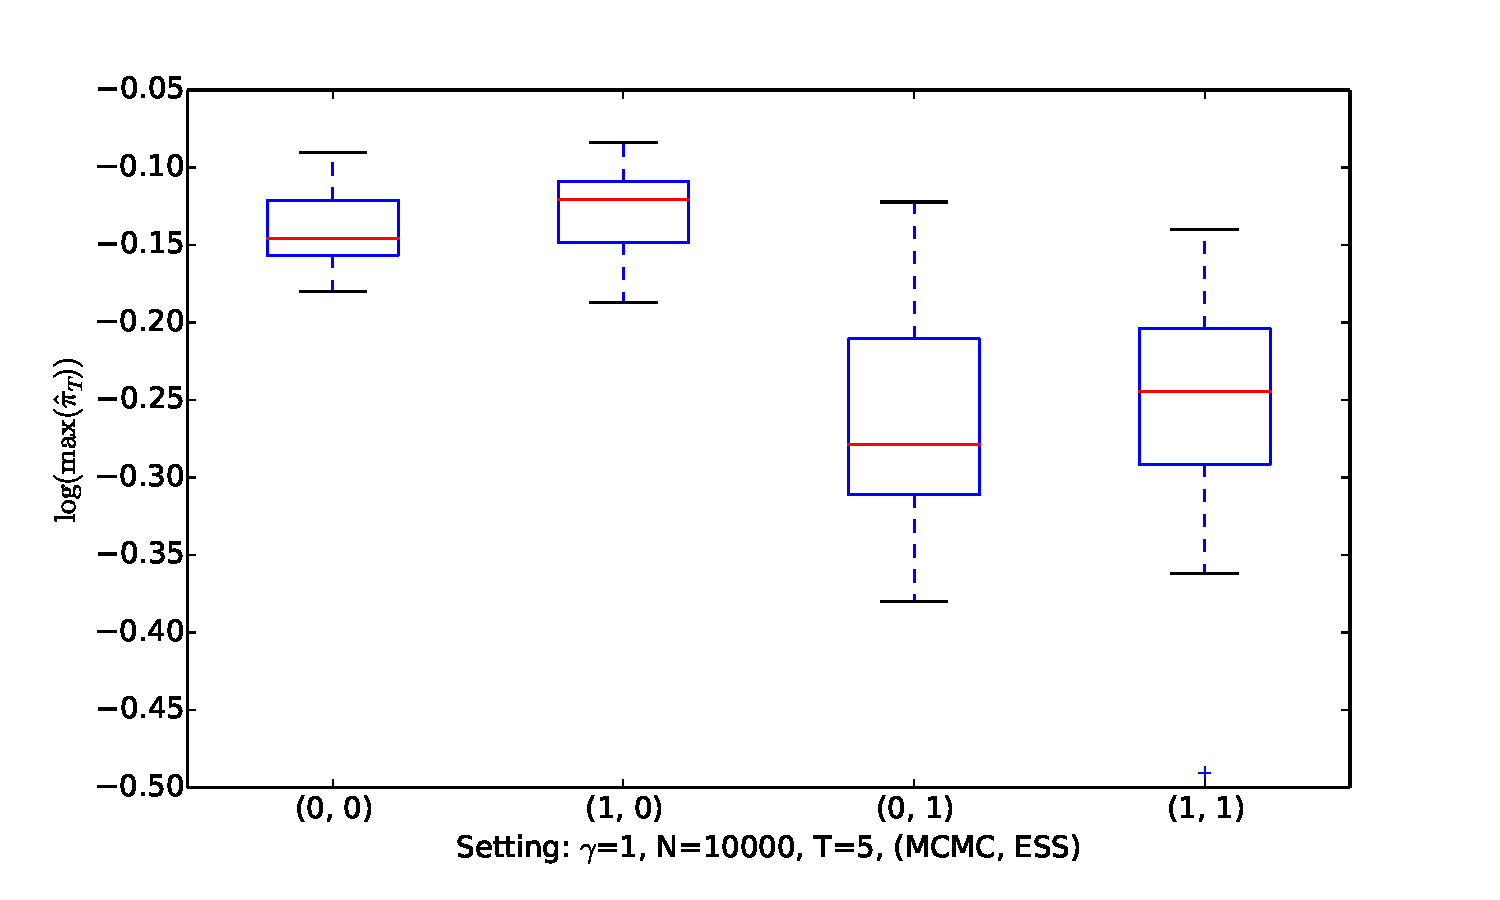
\includegraphics[width=\textwidth]{loglik_mcmc_ess/T5_gamma1_N10000.pdf}
      
        %\includegraphics[width=0.3\linewidth, height=0.15\textheight]{prob1_6_2}
        %\caption{$dt=0.1$}
        %\label{fig:prob1_6_2}
    \end{minipage}%
    \begin{minipage}{0.5\textwidth}
        \centering
        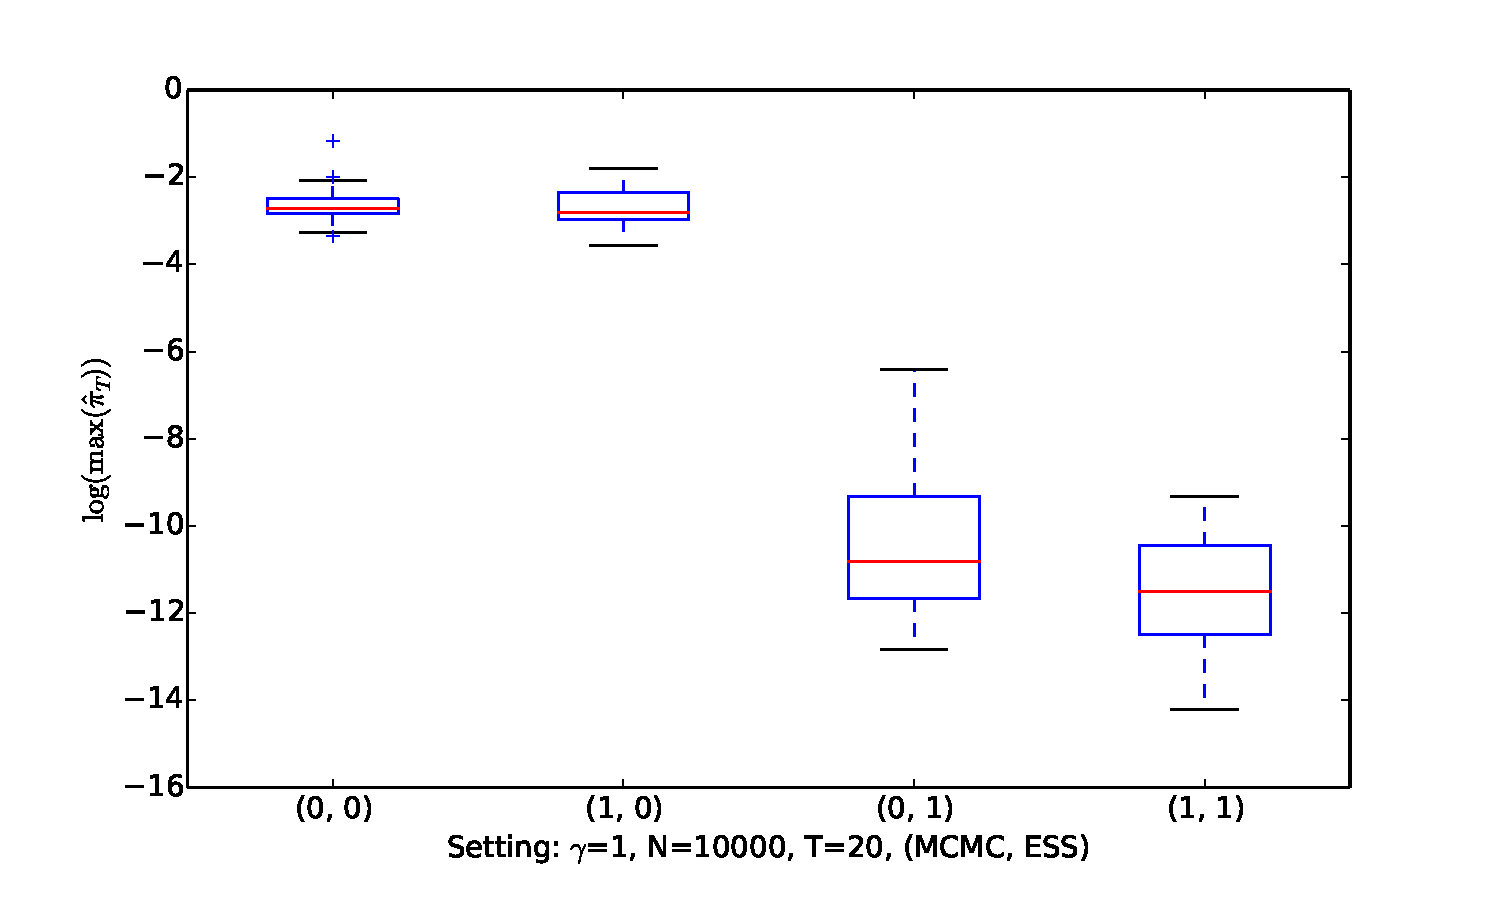
\includegraphics[width=\textwidth]{loglik_mcmc_ess/T20_gamma1_N10000.pdf}
      
    \end{minipage}
    \begin{minipage}{0.5\textwidth}
        \centering
        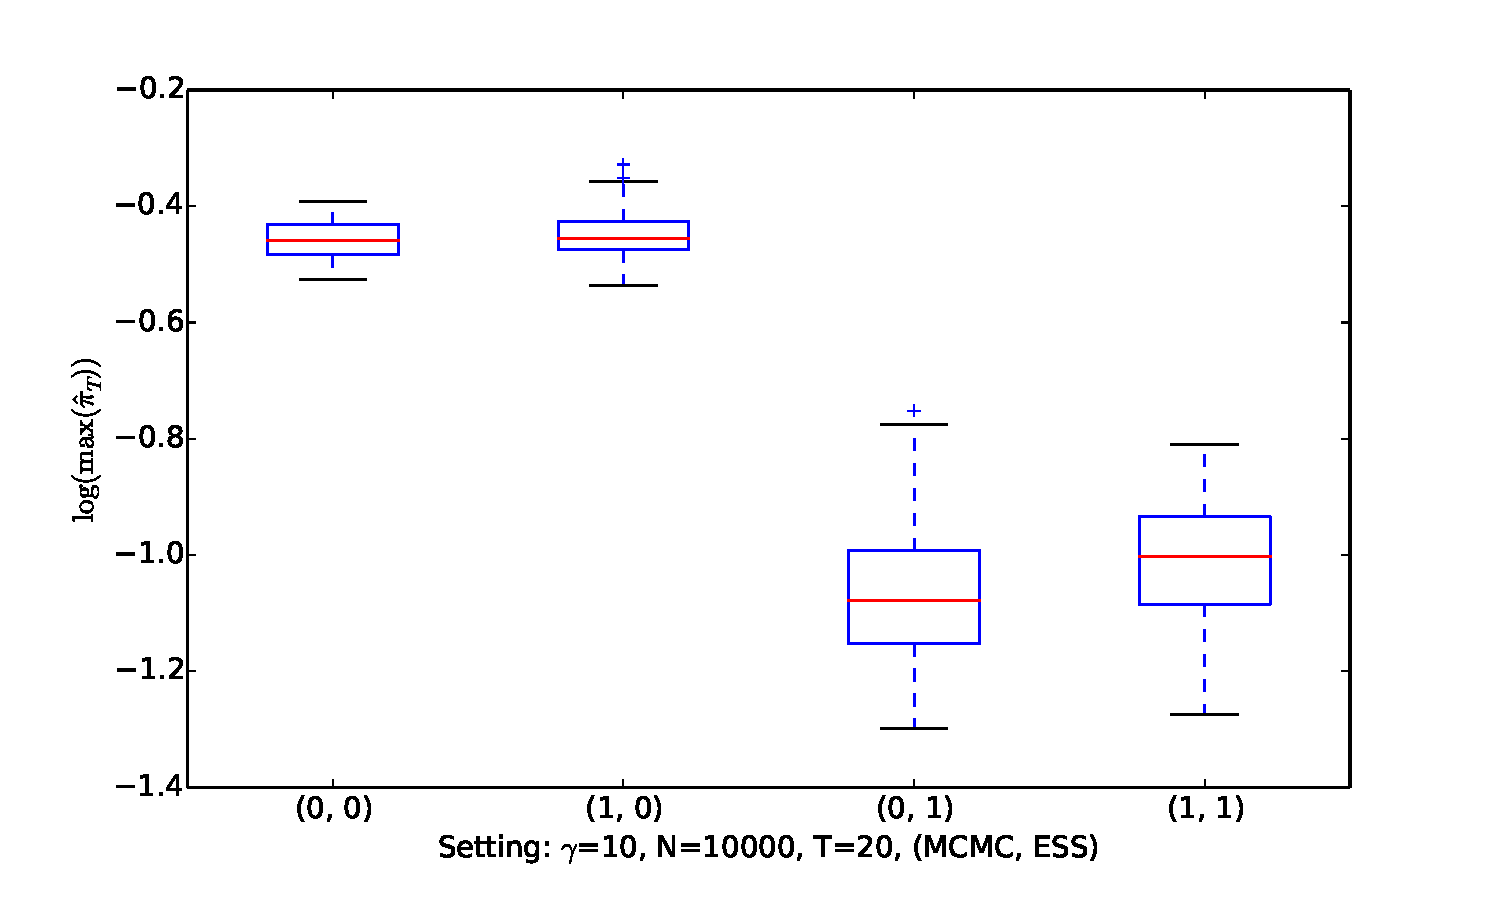
\includegraphics[width=\textwidth]{loglik_mcmc_ess/T20_gamma10_N10000.pdf}
      
    \end{minipage}%
    \begin{minipage}{0.5\textwidth}
        \centering
        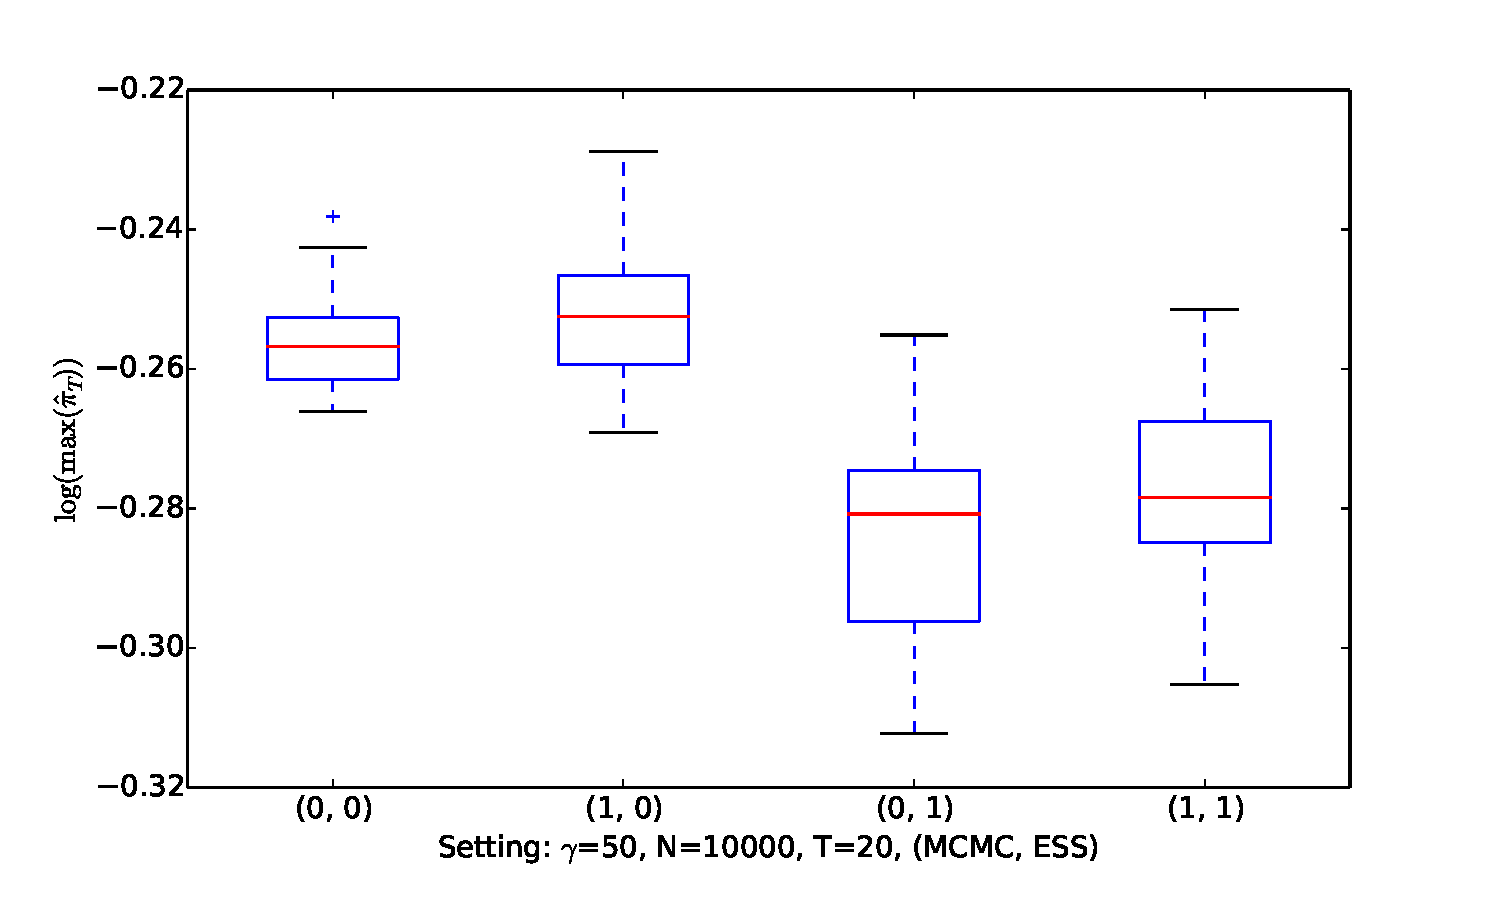
\includegraphics[width=\textwidth]{loglik_mcmc_ess/T20_gamma50_N10000.pdf}
      
    \end{minipage}
    \begin{minipage}{0.5\textwidth}
        \centering
        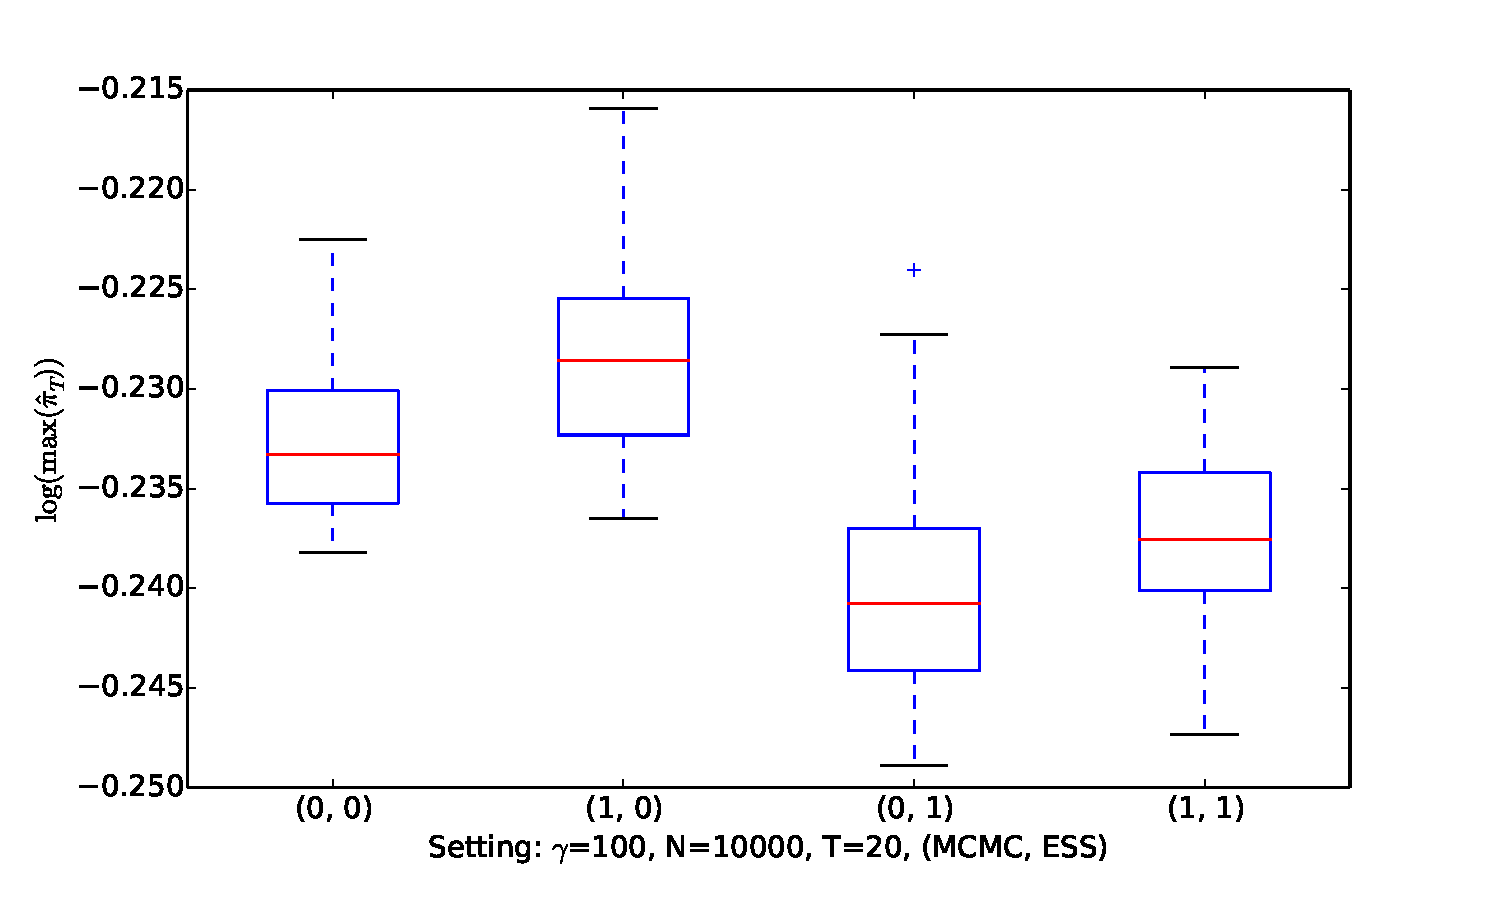
\includegraphics[width=\textwidth]{loglik_mcmc_ess/T20_gamma100_N10000.pdf}
      
    \end{minipage}%
    \begin{minipage}{0.5\textwidth}
        \centering
        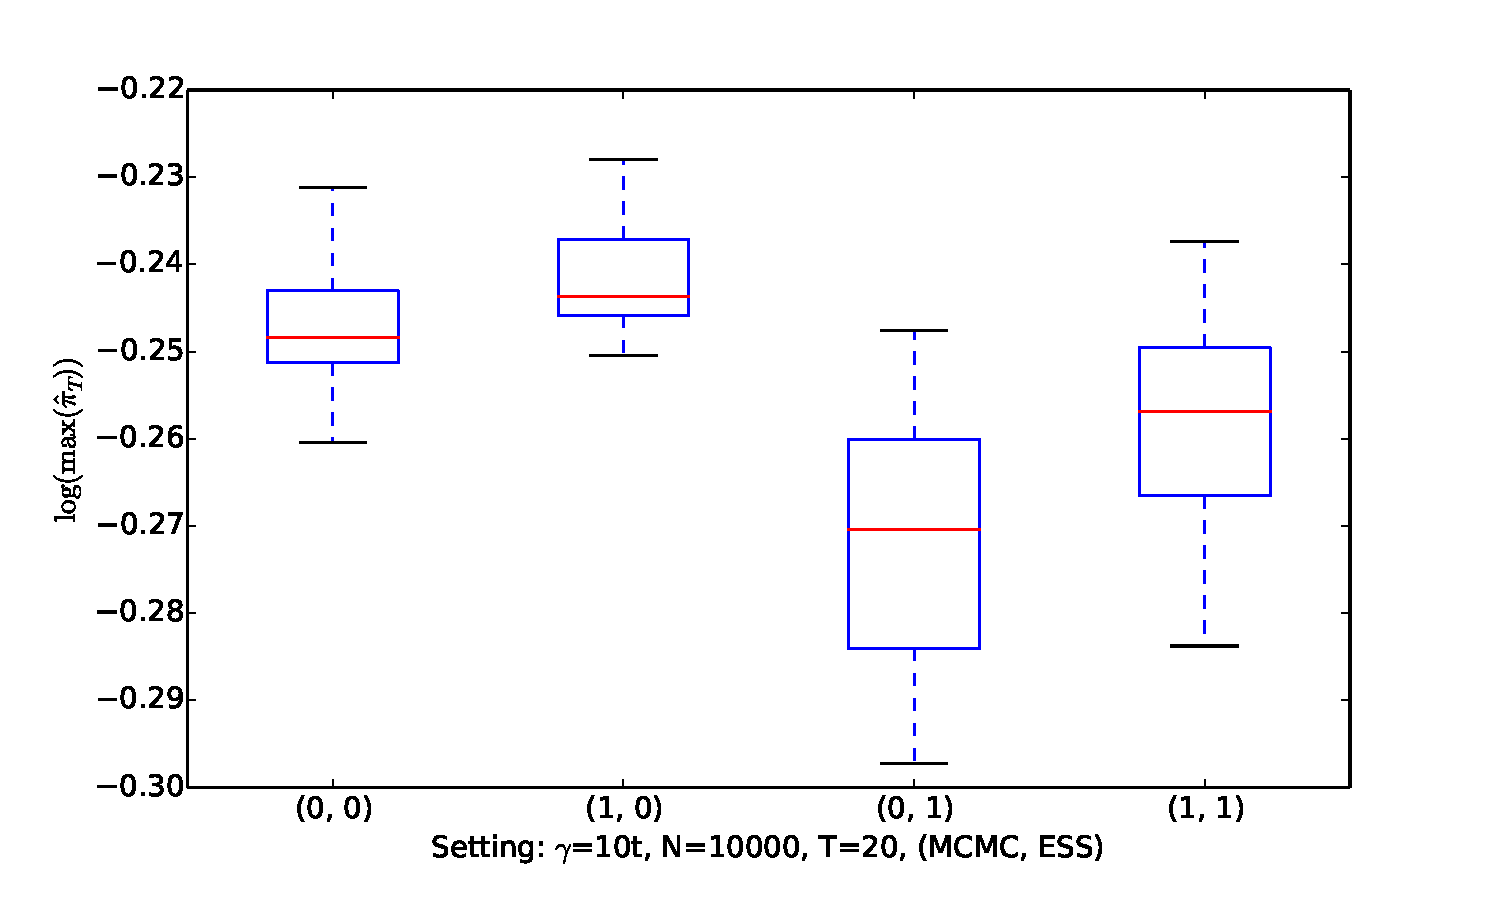
\includegraphics[width=\textwidth]{loglik_mcmc_ess/T20_gamma10t_N10000.pdf}
      
    \end{minipage}
    \begin{minipage}{0.5\textwidth}
        \centering
        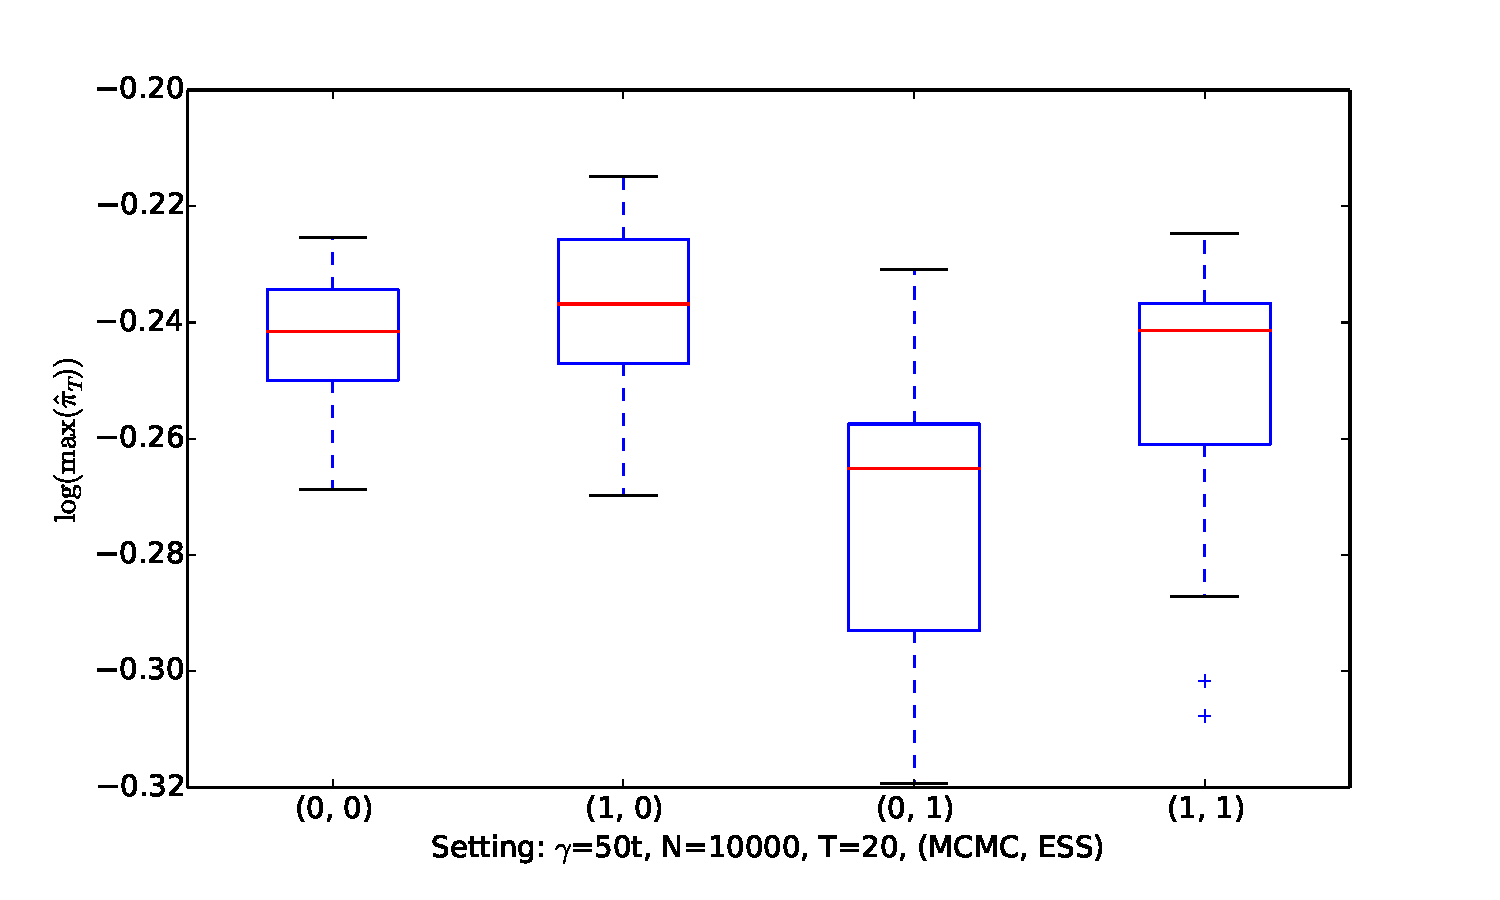
\includegraphics[width=\textwidth]{loglik_mcmc_ess/T20_gamma50t_N10000.pdf}
      
    \end{minipage}%
    \begin{minipage}{0.5\textwidth}
        \centering
        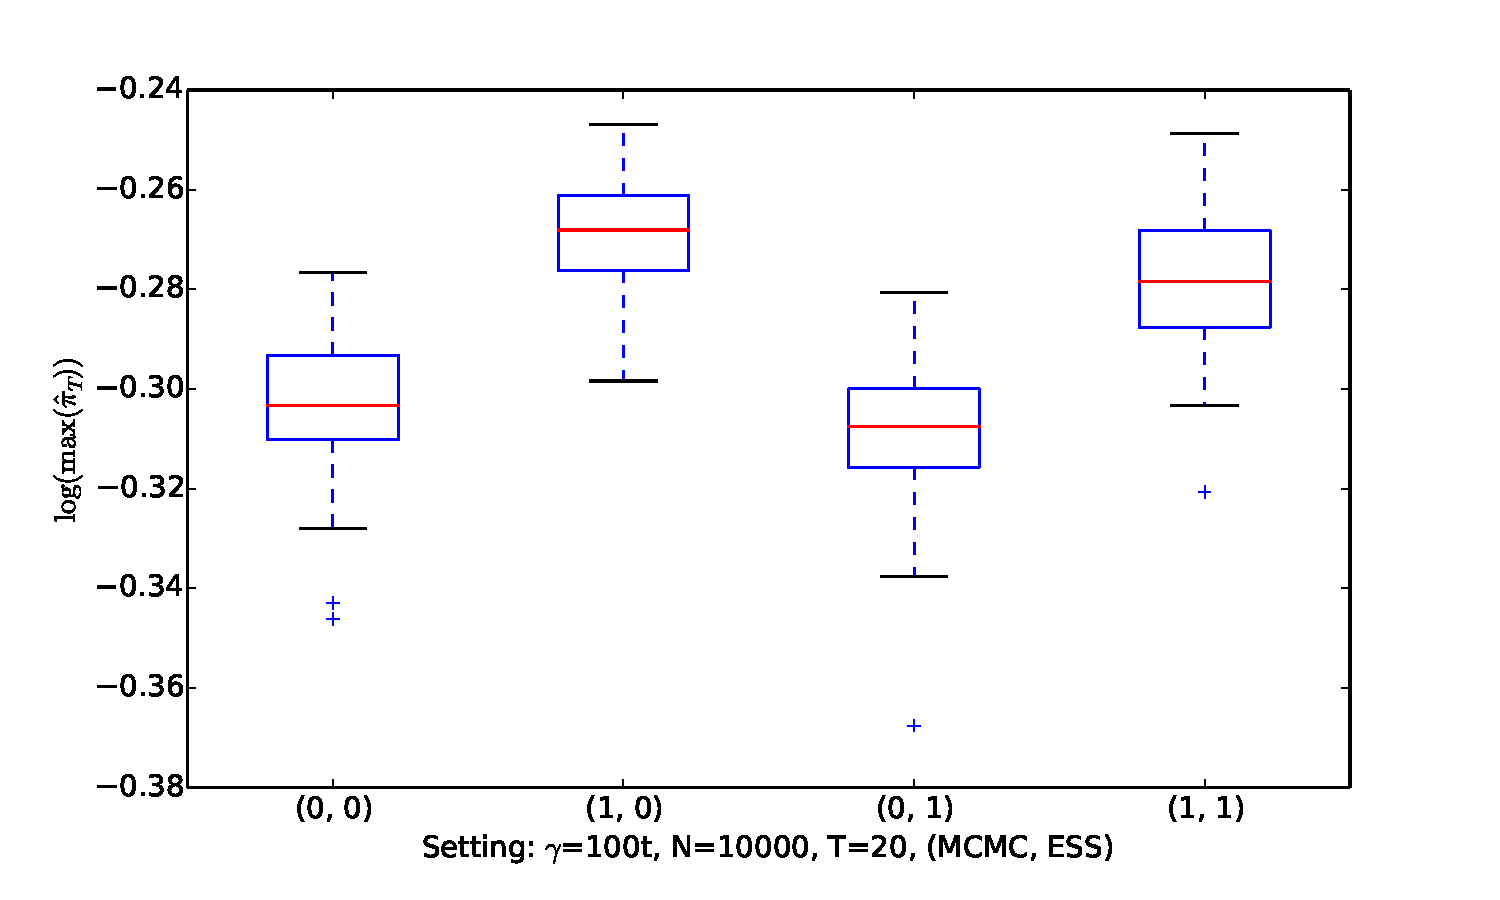
\includegraphics[width=\textwidth]{loglik_mcmc_ess/T20_gamma100t_N10000.pdf}
    \end{minipage}
    \caption{The performance in terms of $\log\pi_T(\hat{u}^*_{1:t})$ of 30 independent runs of the algorithms  with $T=20$ and $N=10000$ for various $\gamma$ settings. The four box-plots in each sub-figure represent the results of runs with the following settings (from left to right): a) MCMC disabled, ESS disabled, b) MCMC enabled, ESS disabled, c) MCMC disabled, ESS enabled, and d) MCMC enabled, ESS enabled.   }
    \label{fig:ess}
\end{figure}

\subsubsection{Resample-Move step with MCMC}
In Figure \ref{fig:ess}, we can also observe that the Resample-Move step does improve performance, albeit the improvement is marginal  in most of the cases. The improvement is more significant when $\gamma$ is set to be high. Figures \ref{fig:rm1}, \ref{fig:rm2} and \ref{fig:rm3} show the box plots of $\log\pi_T(\hat{u}^*_{1:t})$ of $30$ independent runs for time period $T$ of 5, 10, 20 respectively. Each sub-figure shows the runs for a selected $\gamma$ setting with the box-plots grouped by whether the Resample-Move step is used (on the left) or not (on the right), sorted in terms of number of samples used $N$.

One possible explanation to this result is that high $\gamma$ settings sharpen the distribution shape. Such a setting encourages optimisation by pushing the sample towards  high density area but at the same time reduces the space exploration. With excessively high $\gamma$ settings, the sample set may be led to a local optimal with relatively high density area, which may not be the mode of the distribution. The perturbation Resample-Move step introduced at each iteration may help particles to escape from local optimal.

\begin{figure}[!thbp]
    \centering
    \begin{minipage}{.5\textwidth}
        \centering
        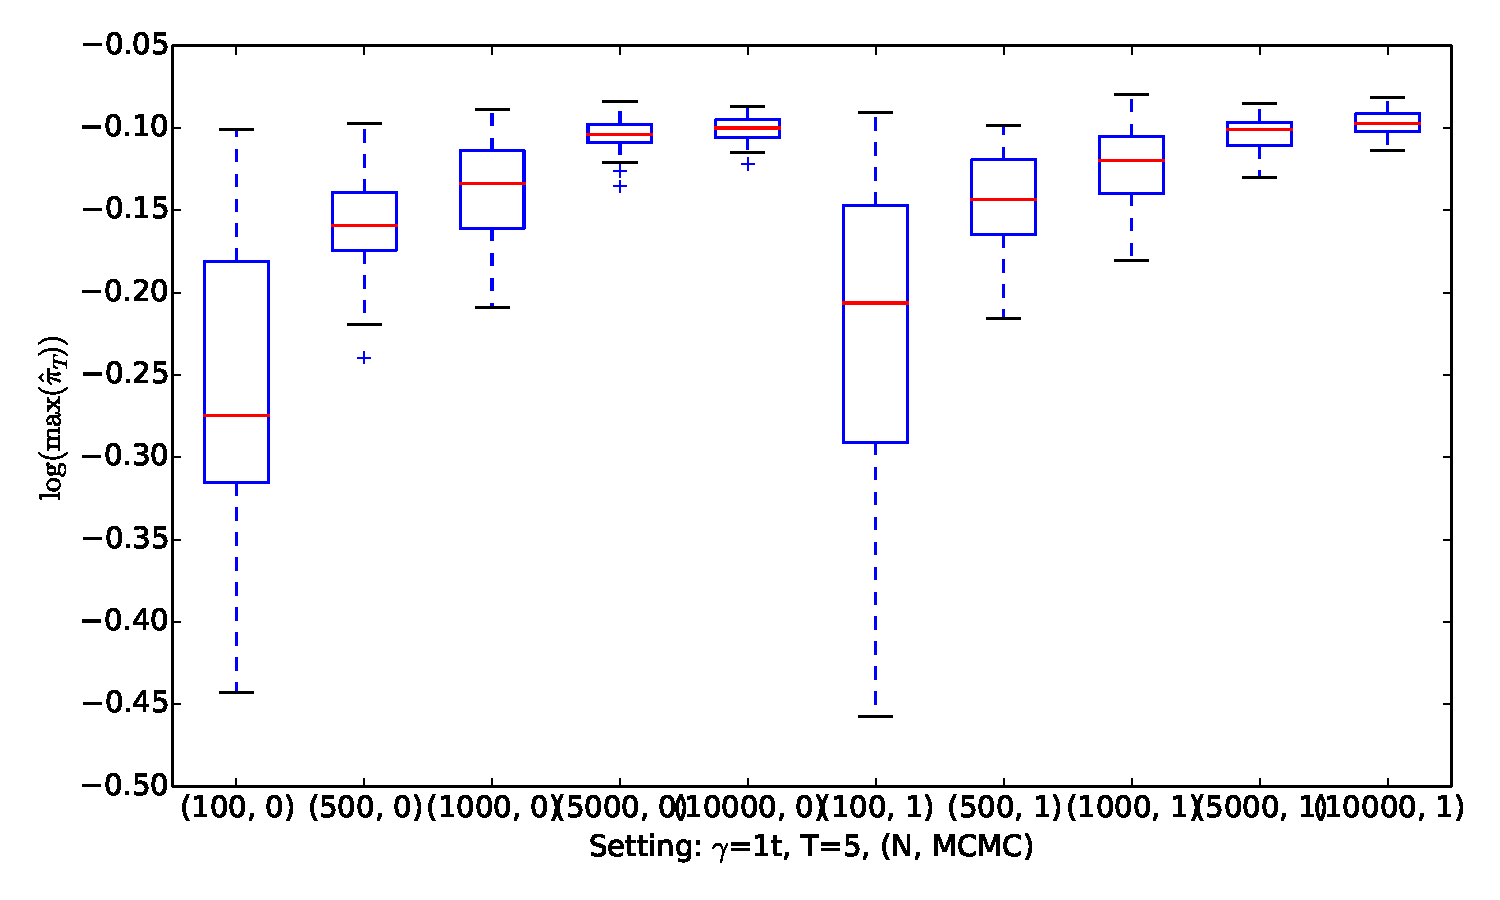
\includegraphics[width=\textwidth]{loglik_t_gs_n/T5_gamma1t.pdf}
    \end{minipage}%
    \begin{minipage}{0.5\textwidth}
        \centering
        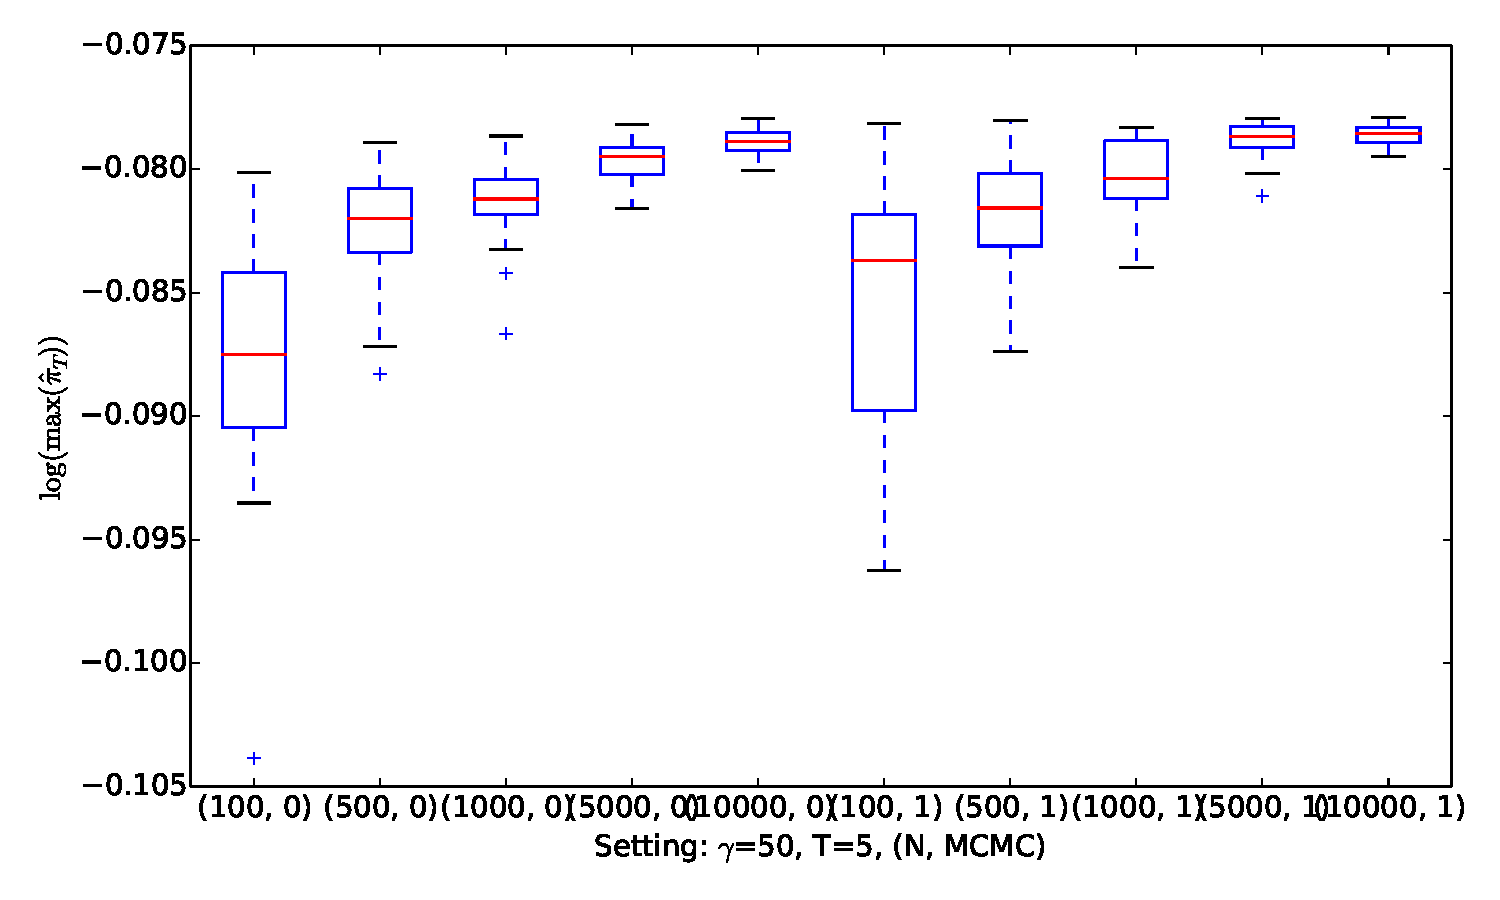
\includegraphics[width=\textwidth]{loglik_t_gs_n/T5_gamma50.pdf}
    \end{minipage}
    \begin{minipage}{0.5\textwidth}
        \centering
        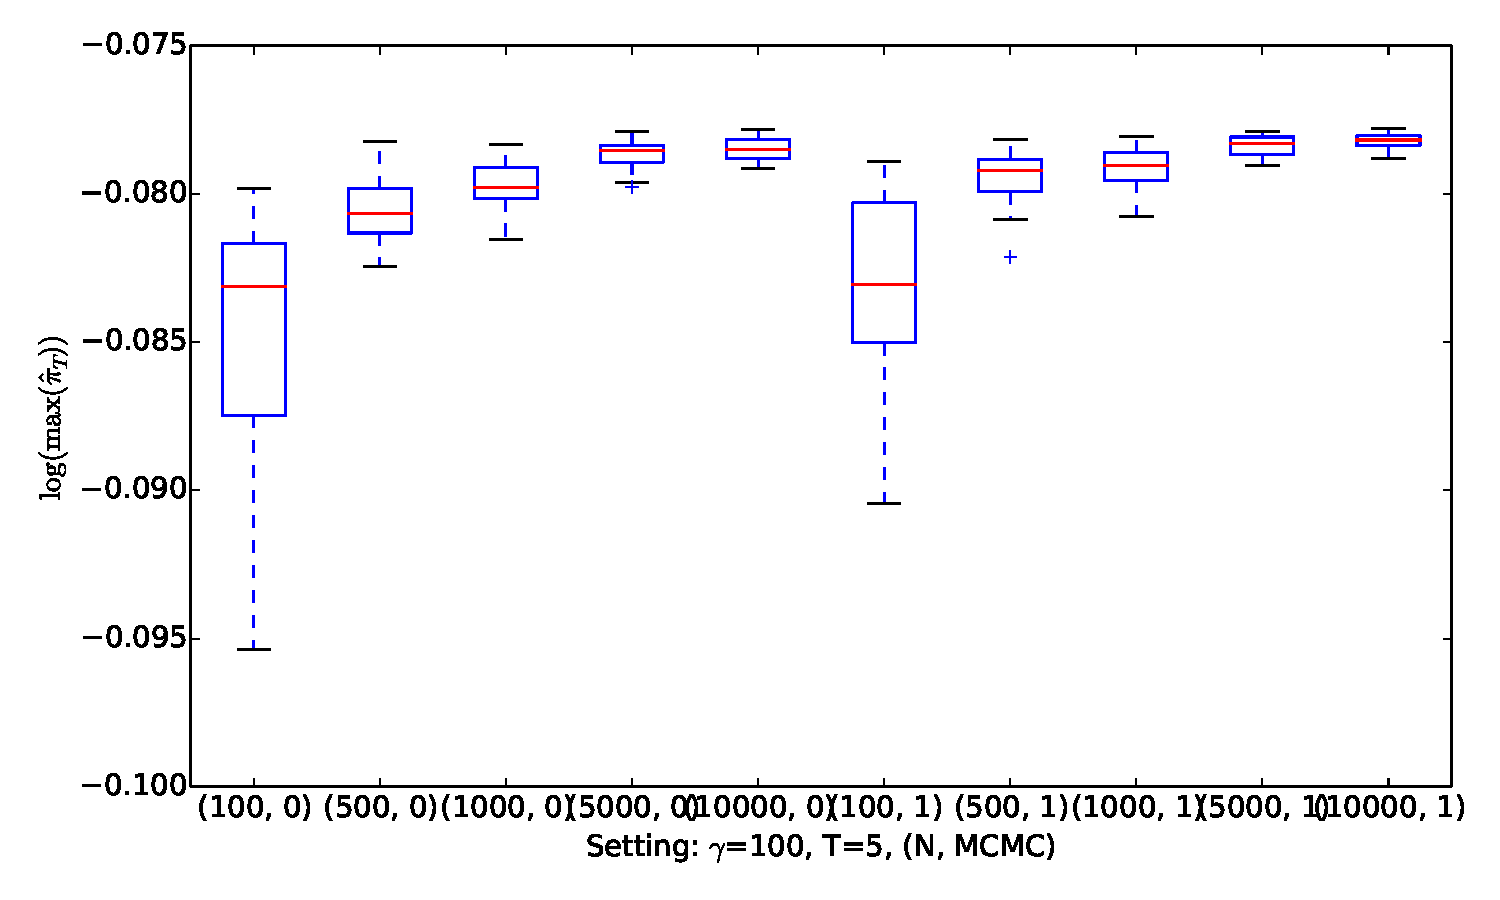
\includegraphics[width=\textwidth]{loglik_t_gs_n/T5_gamma100.pdf}
    \end{minipage}%
    \begin{minipage}{0.5\textwidth}
        \centering
        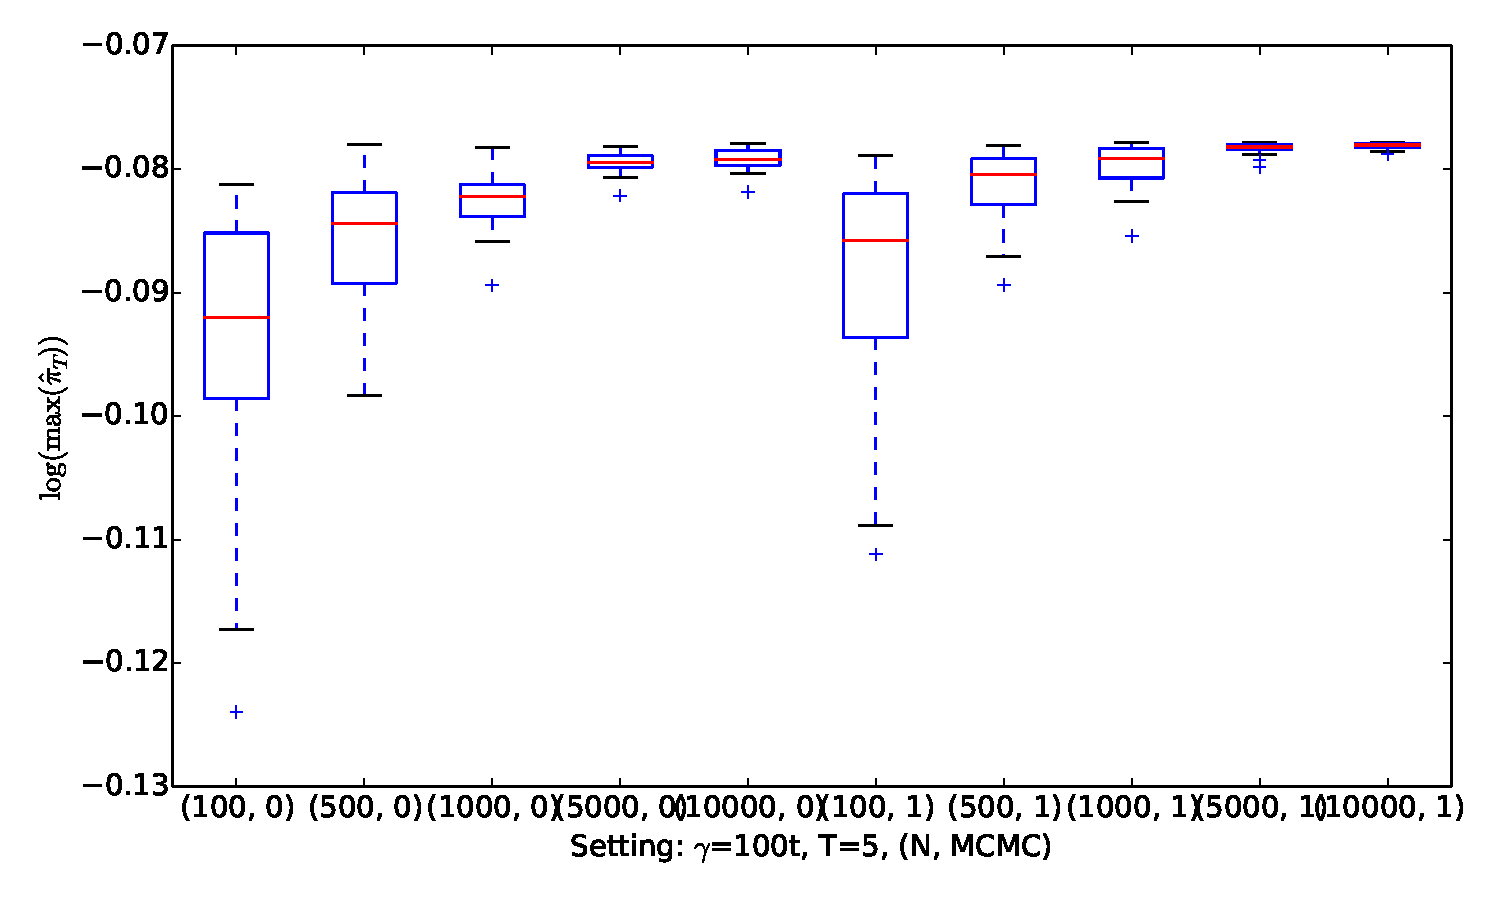
\includegraphics[width=\textwidth]{loglik_t_gs_n/T5_gamma100t.pdf}
    \end{minipage}
    \caption{The $\log\pi_T(\hat{u}^*_{1:t})$ box-plots of 30 independent runs with various settings for $T=5$. Each sub-figure shows the runs for a selected $\gamma$ setting with the box-plots grouped by whether the Resample-Move step is used (on the left) or not (on the right), sorted in terms of number of samples used $N$.}
    \label{fig:rm1}
\end{figure}

\begin{figure}[!thbp]
    \centering
    \begin{minipage}{0.5\textwidth}
        \centering
        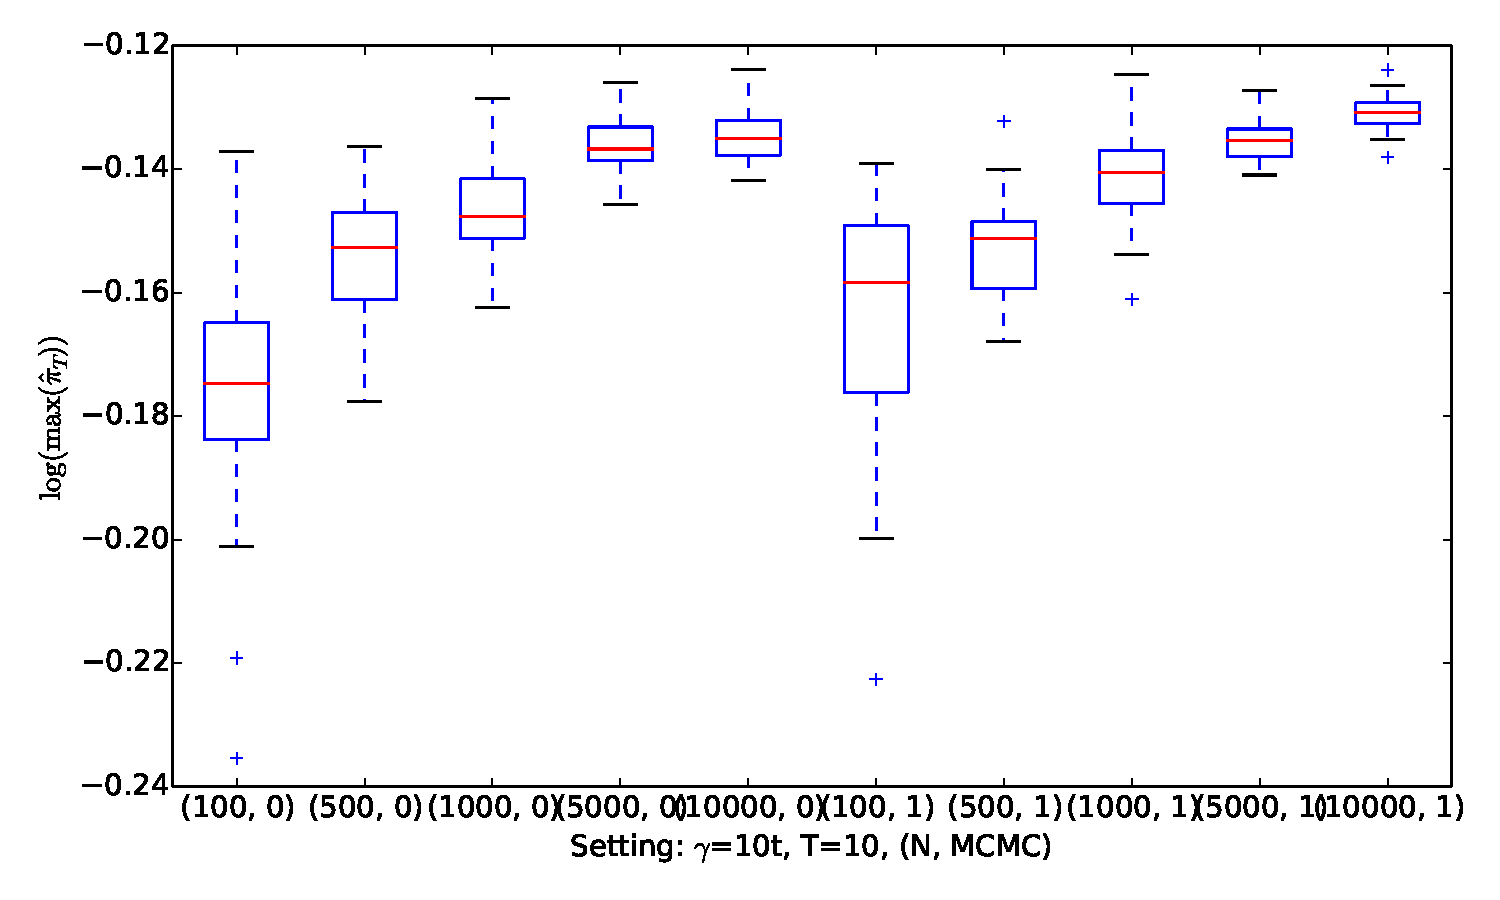
\includegraphics[width=\textwidth]{loglik_t_gs_n/T10_gamma10t.pdf}
    \end{minipage}%
    \begin{minipage}{0.5\textwidth}
        \centering
        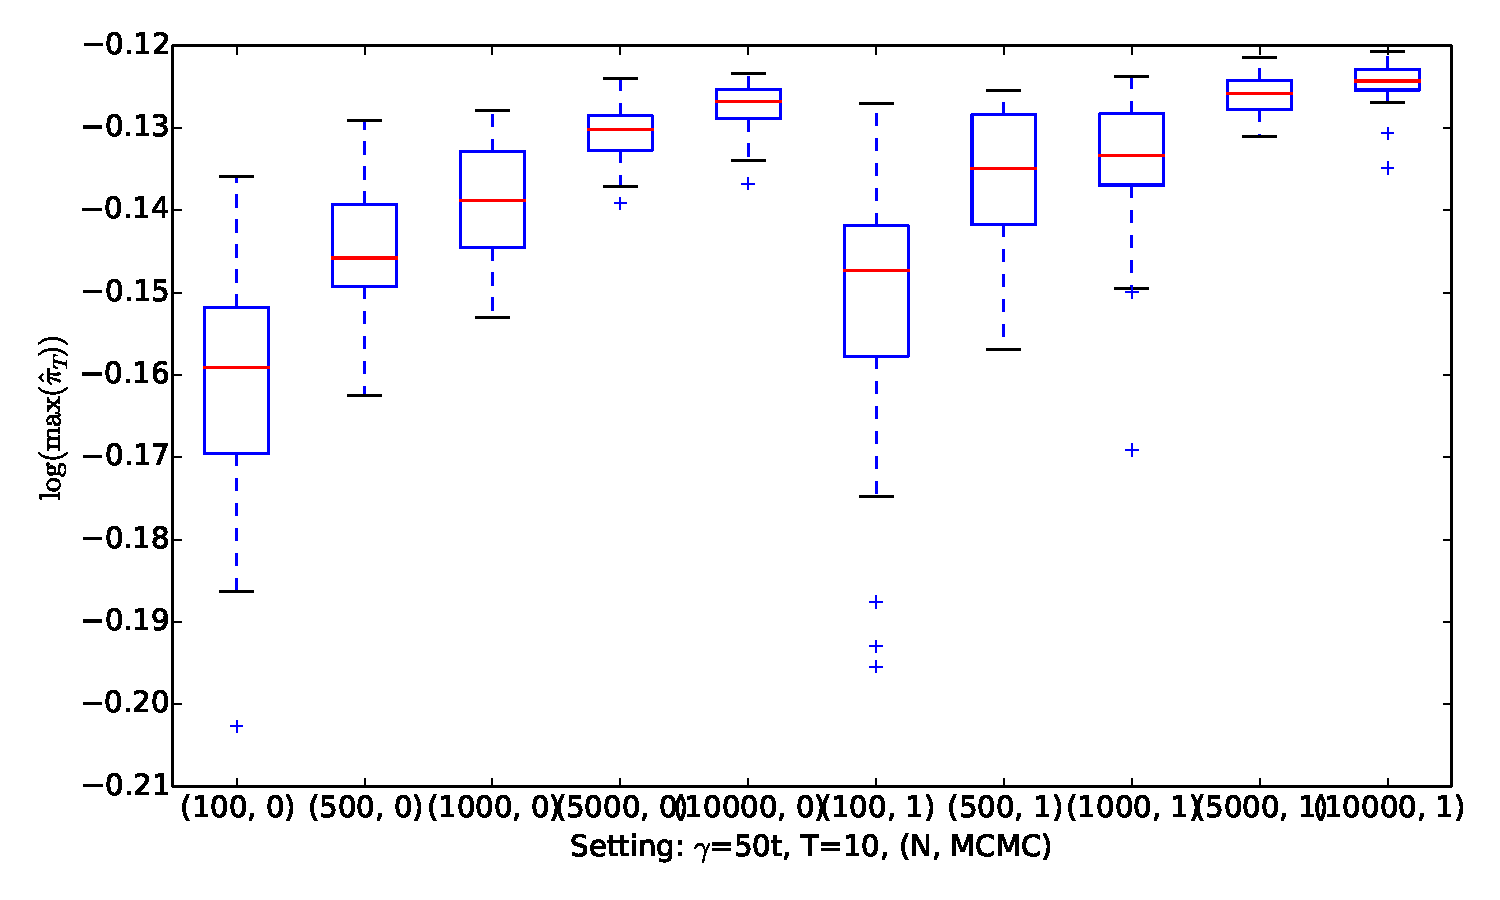
\includegraphics[width=\textwidth]{loglik_t_gs_n/T10_gamma50t.pdf}
    \end{minipage}
    \begin{minipage}{0.5\textwidth}
        \centering
        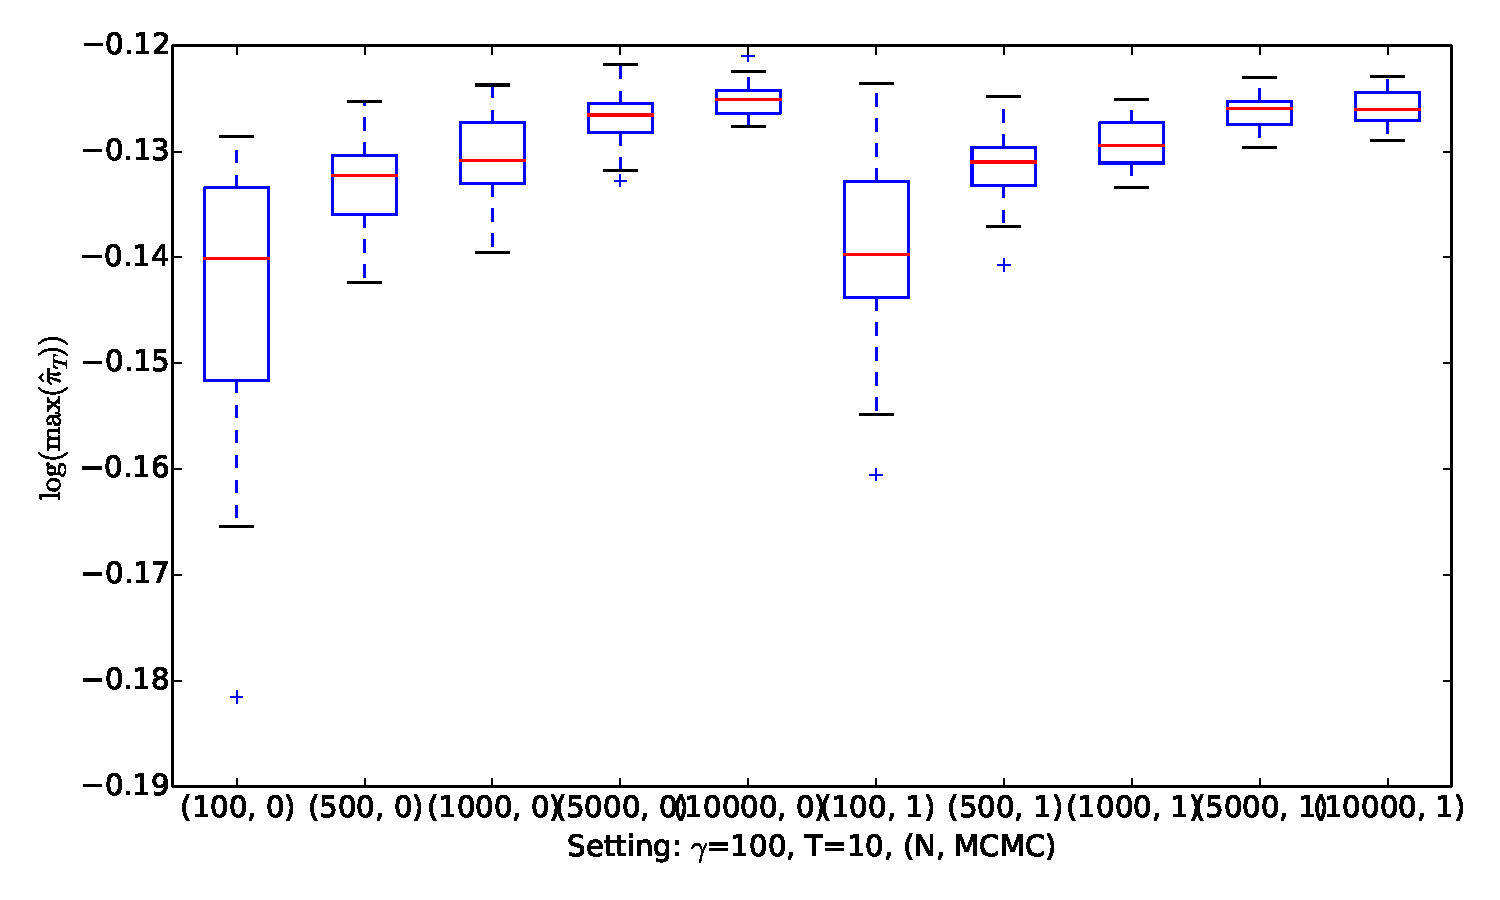
\includegraphics[width=\textwidth]{loglik_t_gs_n/T10_gamma100.pdf}
    \end{minipage}%
    \begin{minipage}{0.5\textwidth}
        \centering
        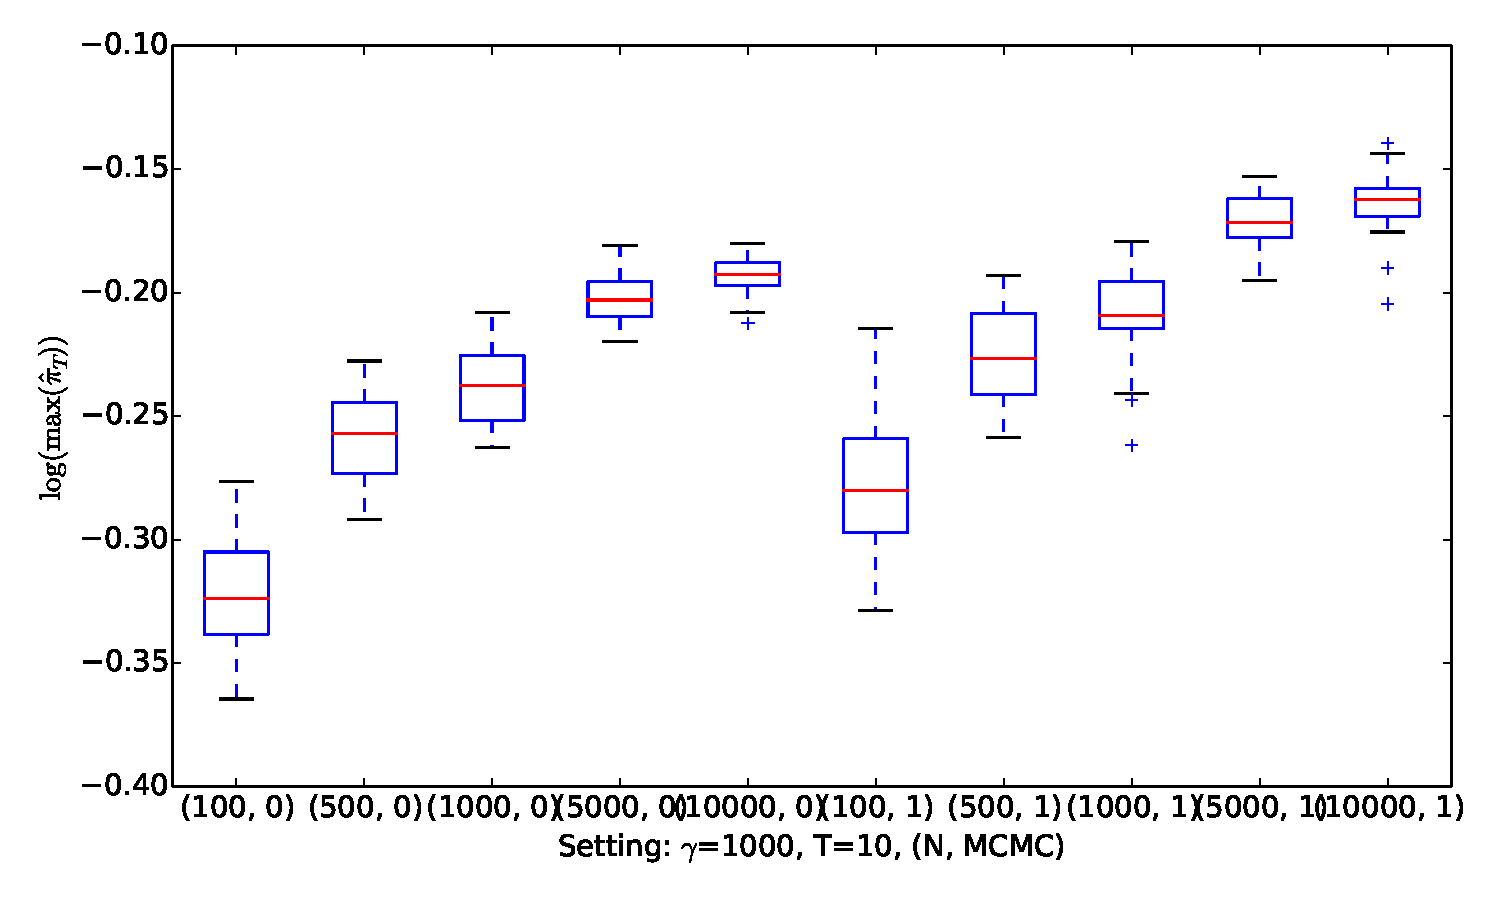
\includegraphics[width=\textwidth]{loglik_t_gs_n/T10_gamma1000.pdf}
    \end{minipage}
    \caption{The $\log\pi_T(\hat{u}^*_{1:t})$ box-plots of 30 independent runs with various settings for $T=10$. Each sub-figure shows the runs for a selected $\gamma$ setting with the box-plots grouped by whether the Resample-Move step is used (on the left) or not (on the right), sorted in terms of number of samples used $N$.}
    \label{fig:rm2}
\end{figure}

\begin{figure}[!thbp]
    \centering
    \begin{minipage}{0.5\textwidth}
        \centering
        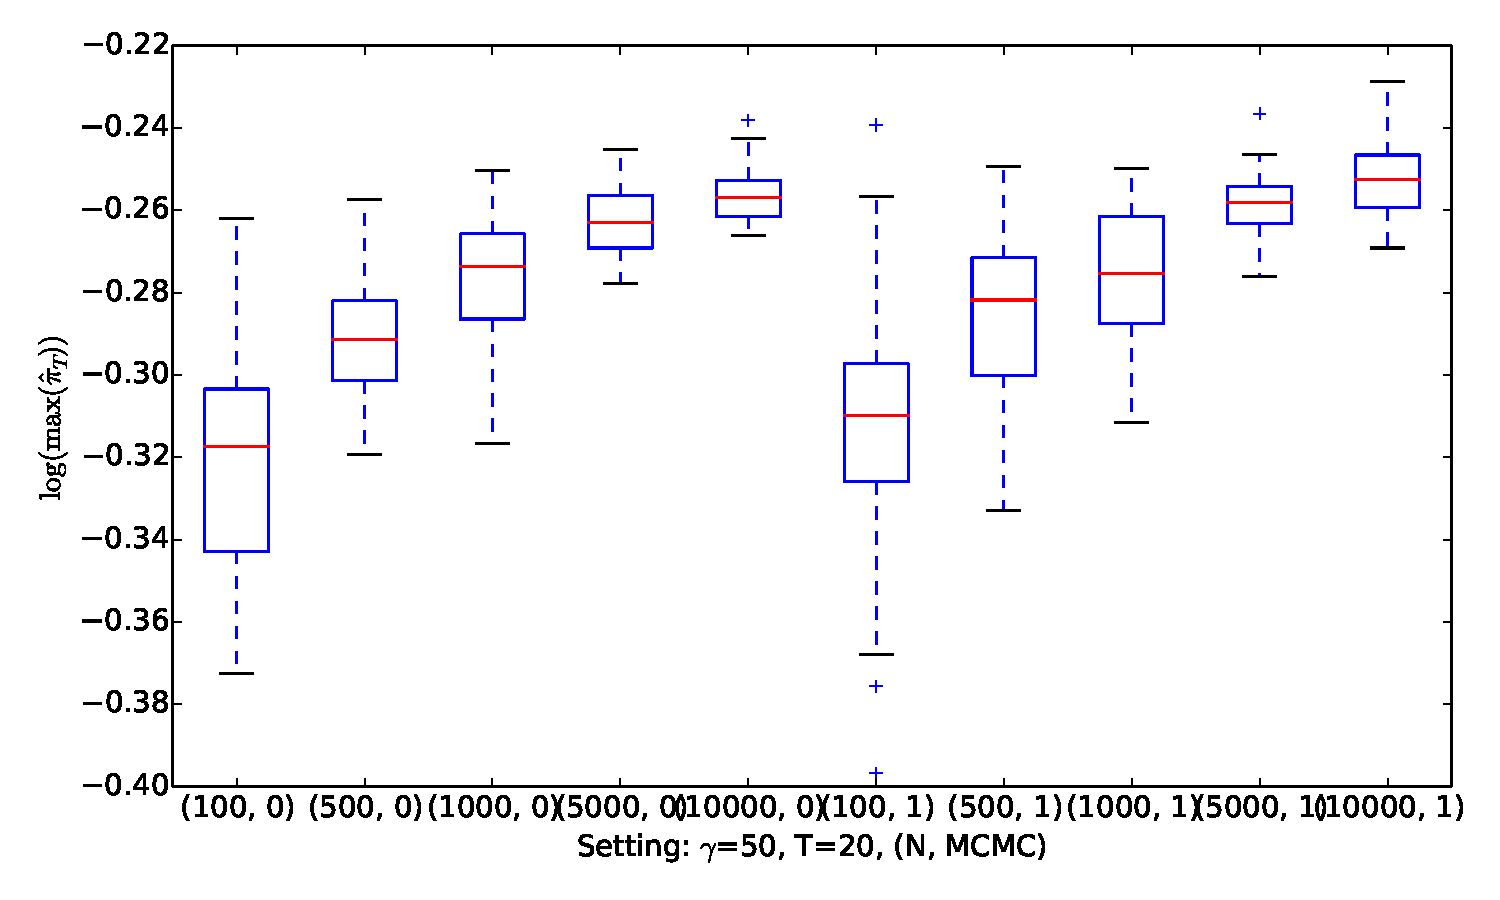
\includegraphics[width=\textwidth]{loglik_t_gs_n/T20_gamma50.pdf}
    \end{minipage}%
    \begin{minipage}{0.5\textwidth}
        \centering
        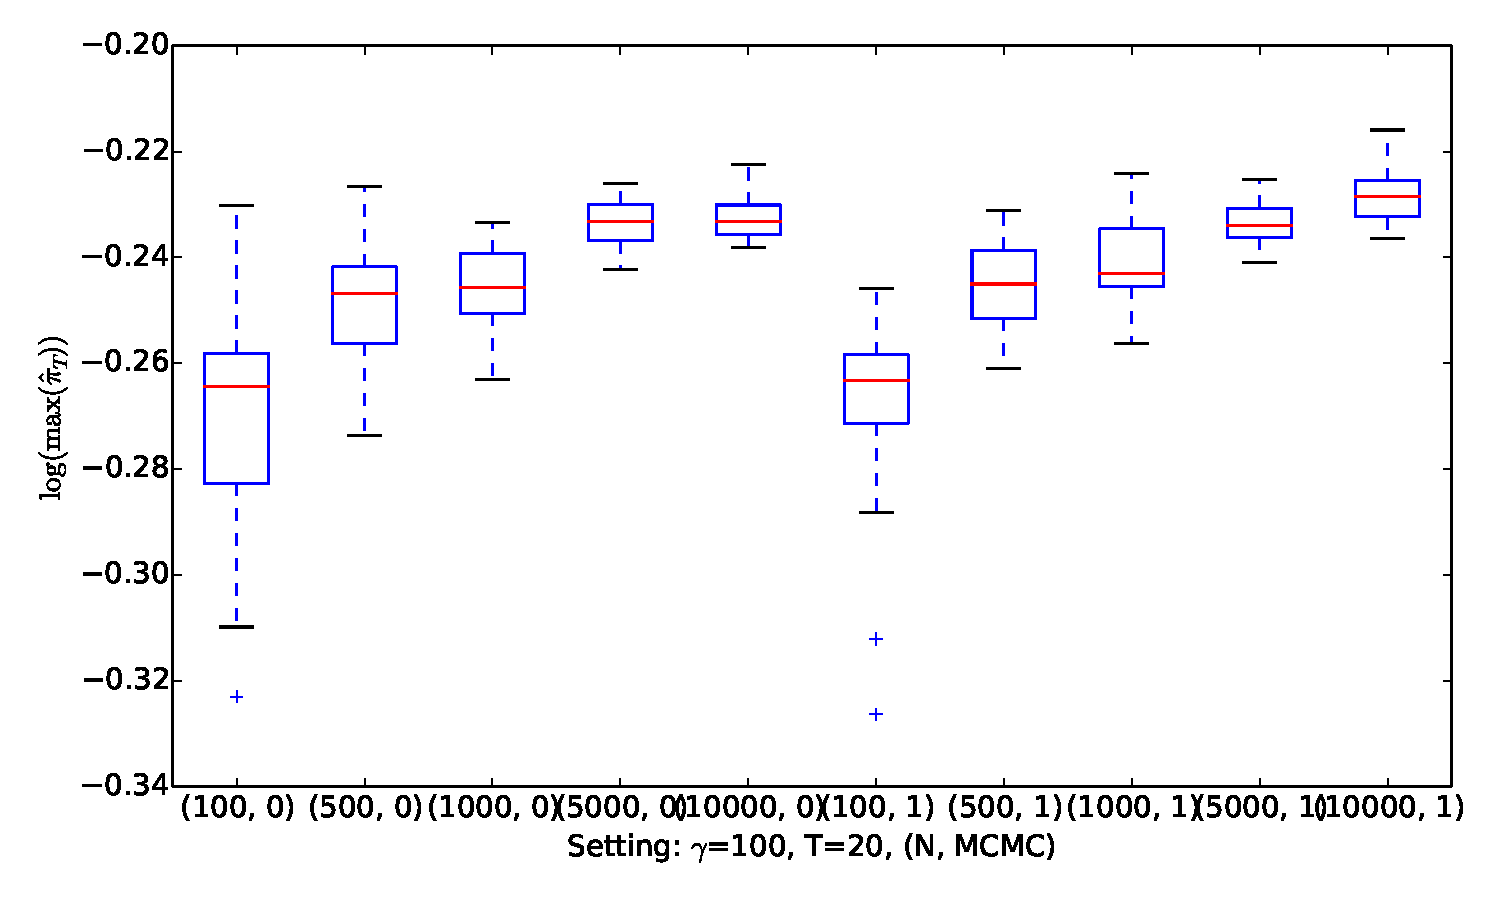
\includegraphics[width=\textwidth]{loglik_t_gs_n/T20_gamma100.pdf}
    \end{minipage}
    \begin{minipage}{0.5\textwidth}
        \centering
        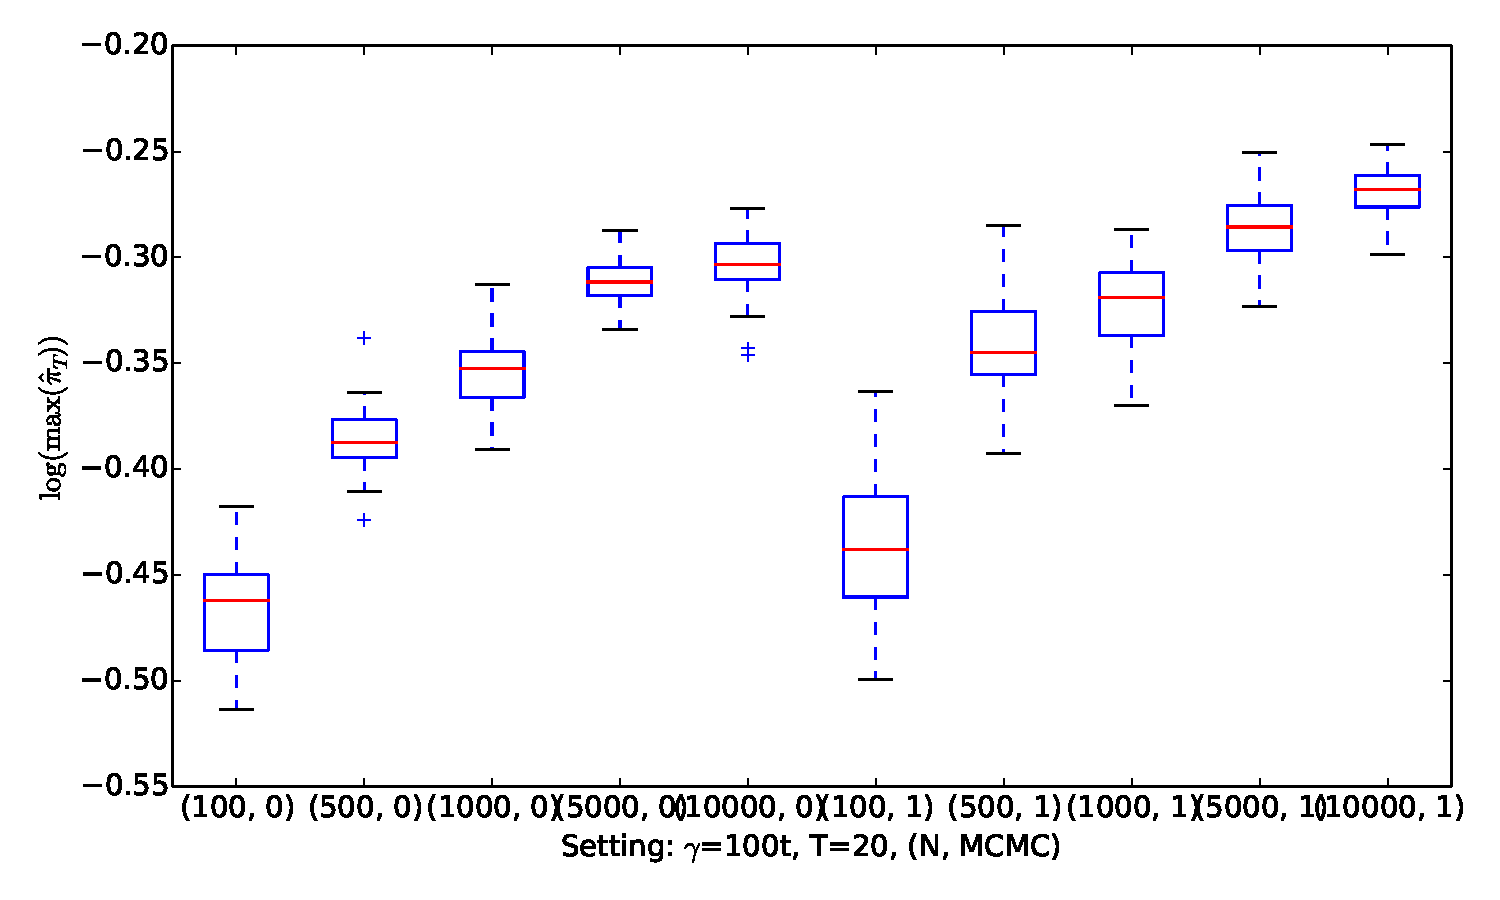
\includegraphics[width=\textwidth]{loglik_t_gs_n/T20_gamma100t.pdf}
    \end{minipage}%
    \begin{minipage}{0.5\textwidth}
        \centering
        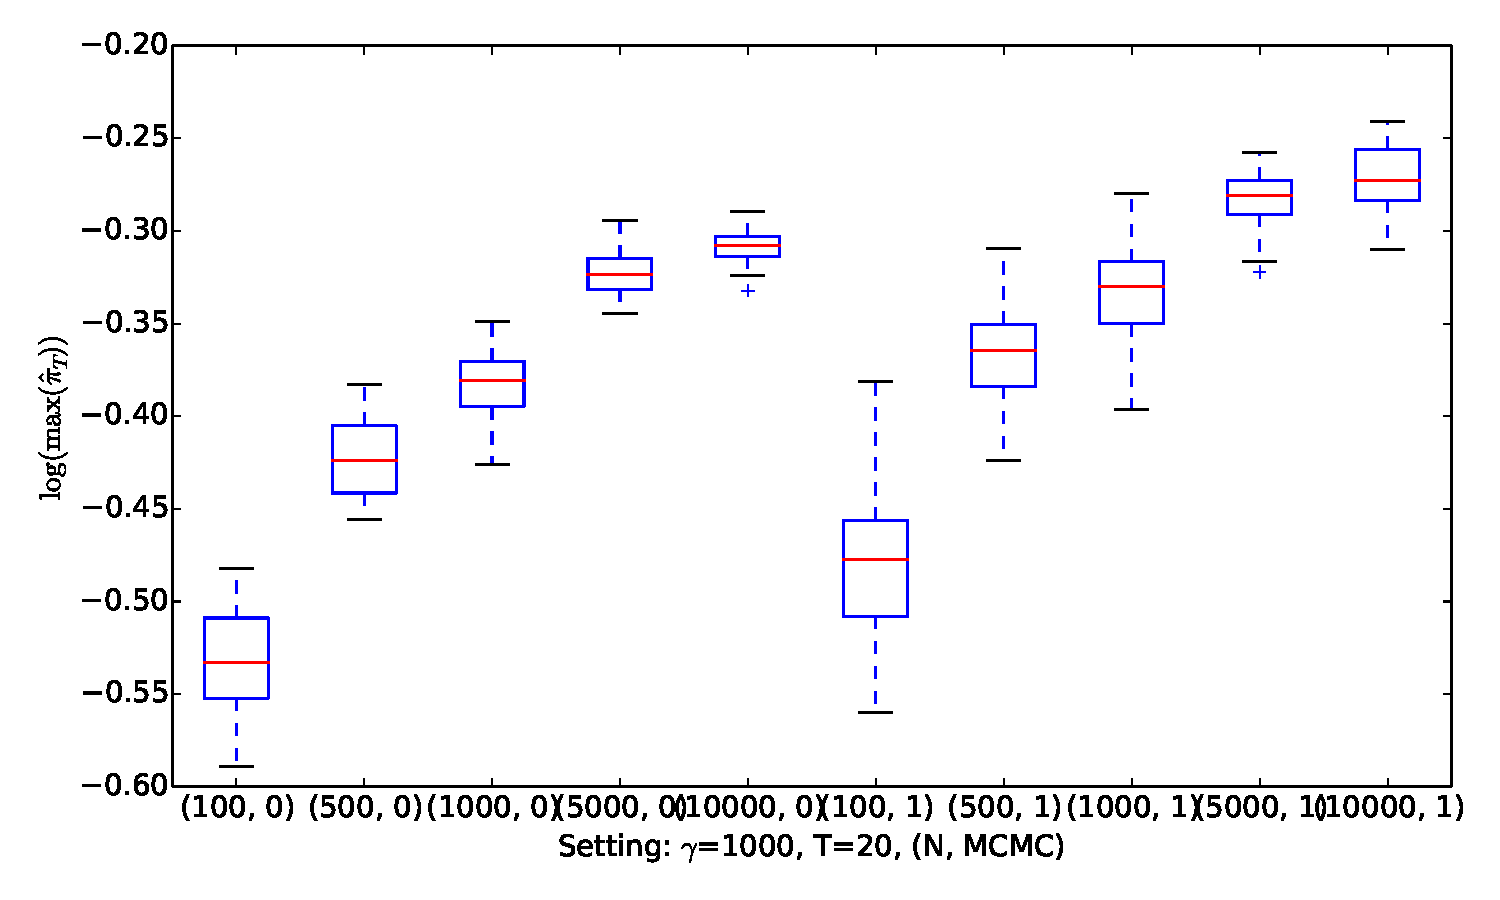
\includegraphics[width=\textwidth]{loglik_t_gs_n/T20_gamma1000.pdf}
    \end{minipage}
    \caption{The $\log\pi_T(\hat{u}^*_{1:t})$ box-plots of 30 independent runs with various settings for $T=20$. Each sub-figure shows the runs for a selected $\gamma$ setting with the box-plots grouped by whether the Resample-Move step is used (on the left) or not (on the right), sorted in terms of number of samples used $N$.}
    \label{fig:rm3}
\end{figure}

\subsubsection{Various sample size settings}
In terms of the sample size setting used, the performance increased monotonically with the number of samples used for all time periods considered as shown in Figures \ref{fig:rm1}, \ref{fig:rm2} and \ref{fig:rm3}. This is in-line with the theory, more samples is always better. For the shorter time-period considered, says $T=5$, the performance improvement sometimes is ``saturated'' even with lower number of samples, says $T=1000$ or $T=5000$. This suggests the optimal control parameters may have been attained.

 \subsubsection{Various $\gamma$ settings}
A more interesting result is to compare the performance with different $\gamma$ settings. Let first consider the fixed $\gamma$ settings. Excessive high $\gamma$ settings may lead to issue discussed earlier and stuck at local optimal. On the other hand, low $\gamma$ settings also does not perform too well either (consider the process of searching for the mode by randomly sampling a very flat distribution). The optimal $\gamma$ setting seems to lie sometimes in between. In this case, the $\gamma=100$ setting results in the best performance.

In \cite{NK11}, it was suggested that using an increasing $\gamma$ setting may be a good pragmatic compromise between accuracy and good mixing. We investigate further on this by setting $\gamma$ to be increasing function of the form $\alpha t$, where $\alpha$ is constant and $t$ is the time step. The results show that the performance seems improve when the $\alpha$ value is low, but the result is worse when the $\alpha$ value is high. This suggests a capping on the maximum value on $\alpha$ or a more moderate in $t$ may be more suitable. We therefore carry out two extra $\gamma$ settings: $50\log(t+1)$ and $100\log(t+1)$ to investigate this. The results of these runs are shown in Figure \ref{fig:log}. The results obtained are not statistically different from a simple fixed $\gamma=100$ setting.

\begin{figure}[!thbp]
    \centering
    \begin{minipage}{.5\textwidth}
        \centering
        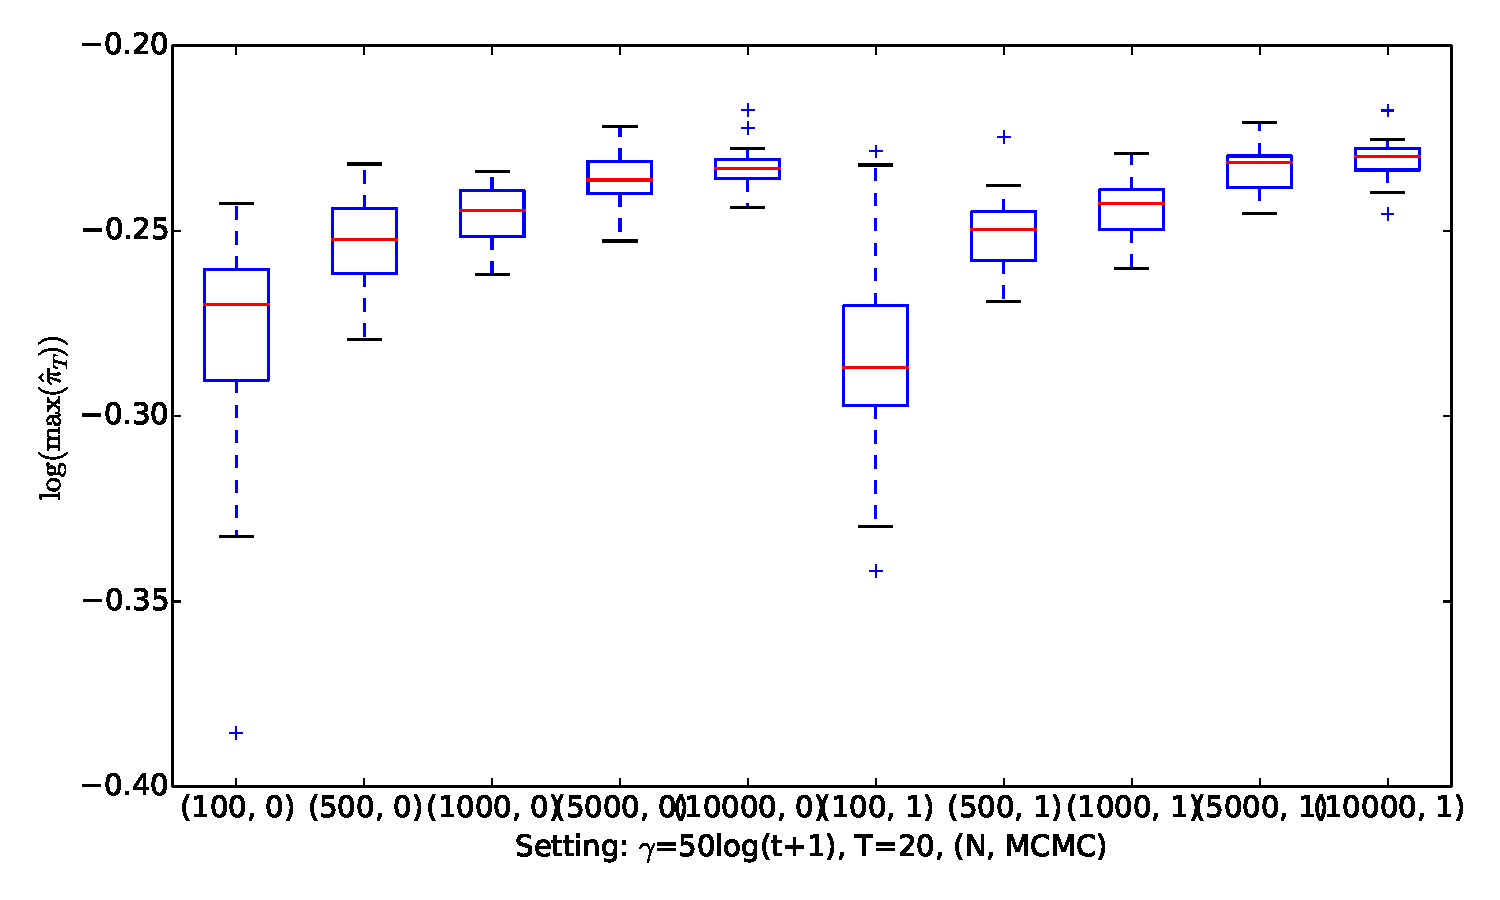
\includegraphics[width=\textwidth]{loglik_t_gs_n/T20_gamma50log(t+1).pdf}
        %\includegraphics[width=0.3\linewidth, height=0.15\textheight]{prob1_6_2}
        %\caption{$dt=0.1$}
        %\label{fig:prob1_6_2}
    \end{minipage}%
    \begin{minipage}{0.5\textwidth}
        \centering
        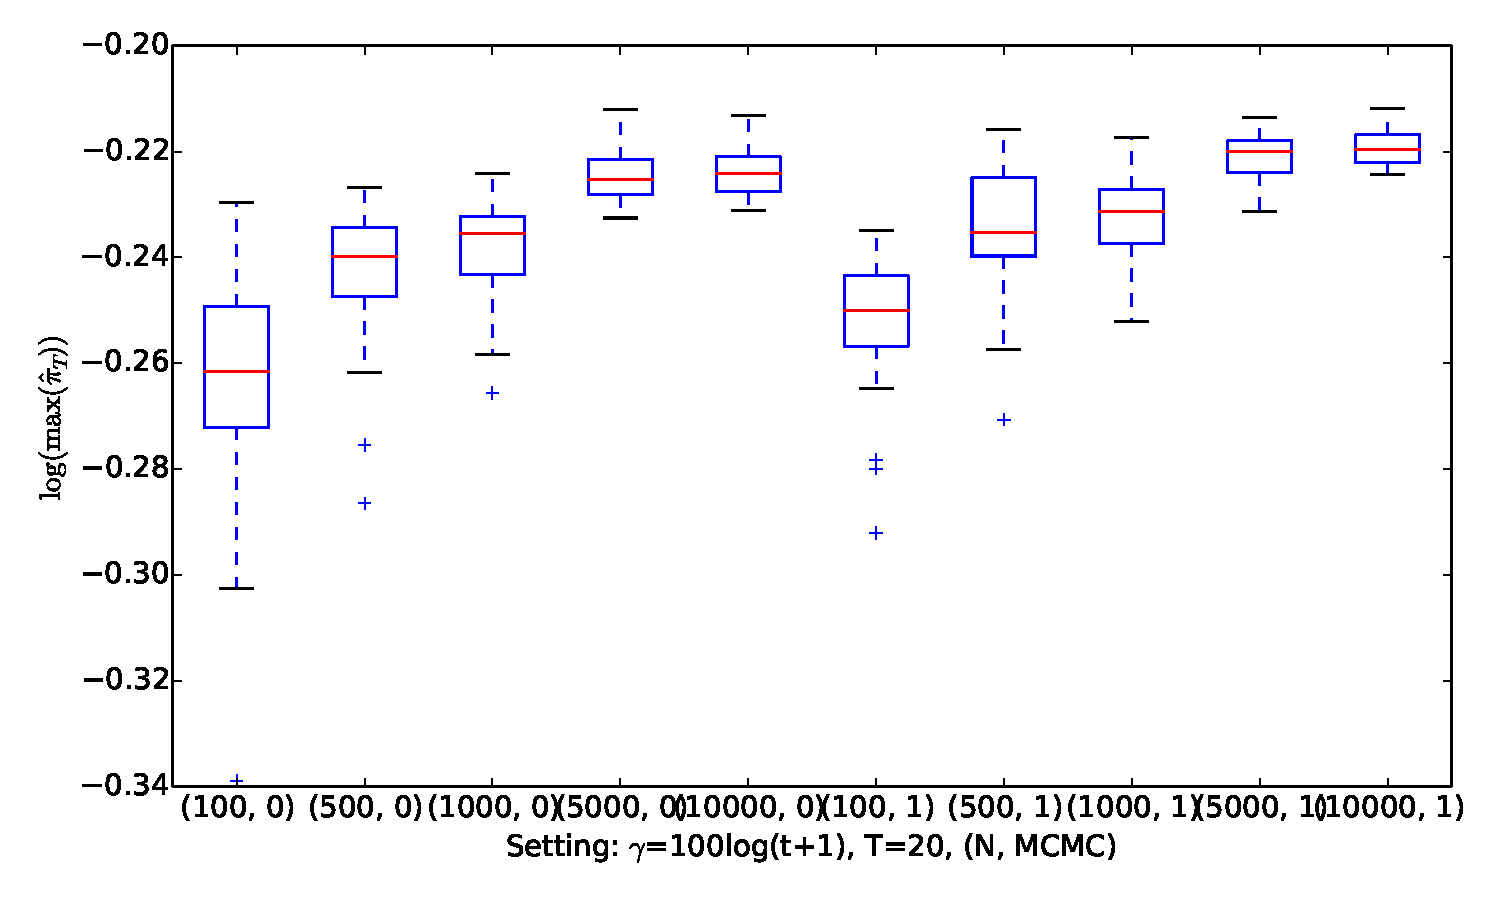
\includegraphics[width=\textwidth]{loglik_t_gs_n/T20_gamma100log(t+1).pdf}
    \end{minipage}
    \caption{The $\log\pi_T(\hat{u}^*_{1:t})$ box-plots of 30 independent runs with $\gamma$ settings: $50\log(t+1)$ and $100\log(t+1)$. Each sub-figure shows the runs for a selected $\gamma$ setting with the box-plots grouped by whether the Resample-Move step is used (on the left) or not (on the right), sorted in terms of number of samples used $N$.}
    \label{fig:log}
\end{figure}

Lastly, we conclude this section by showing the mean of the recursive likelihood $m_{t \mid t-1}(u^*_{1:T})$ obtained in various runs in Figure \ref{fig:estimatedy} and their corresponding tracking errors in Figure \ref{fig:error}. The results looks very promising. Except in the runs with the $\gamma=1$ setting in which there is a lot of noise in tracking, all other runs are able to closely track the reference signal. 

\begin{figure}[!thbp]
    \centering
    \begin{minipage}{.5\textwidth}
        \centering
        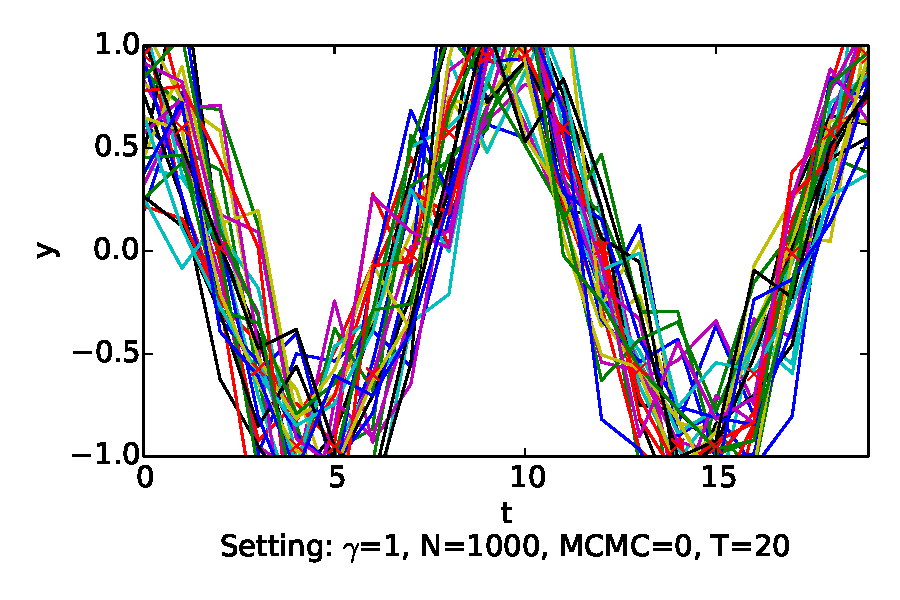
\includegraphics[width=\textwidth]{output_y/output_20_1.pdf}
    \end{minipage}%
    \begin{minipage}{0.5\textwidth}
        \centering
        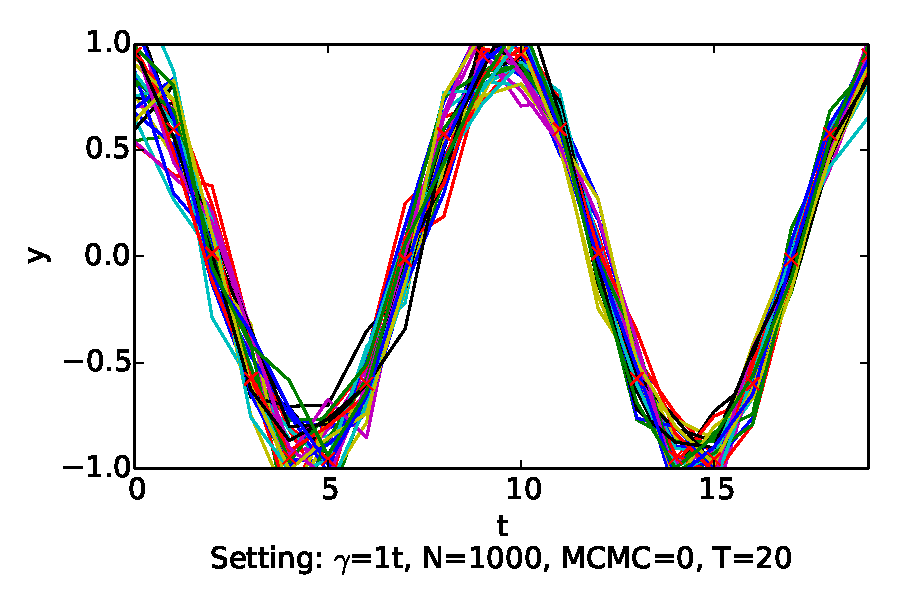
\includegraphics[width=\textwidth]{output_y/output_20_1t.pdf}
    \end{minipage}
    \begin{minipage}{0.5\textwidth}
        \centering
        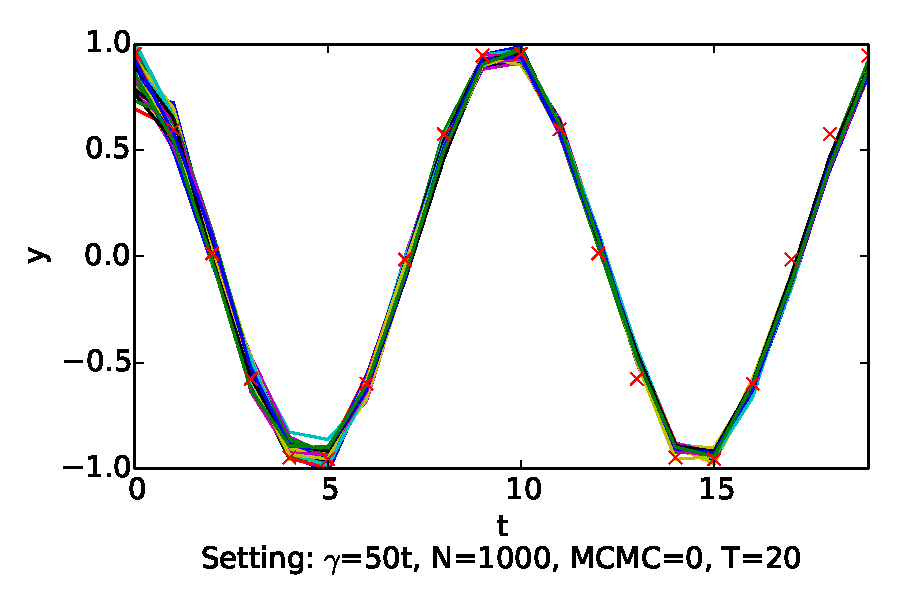
\includegraphics[width=\textwidth]{output_y/output_20_50t.pdf}
    \end{minipage}%
    \begin{minipage}{0.5\textwidth}
        \centering
        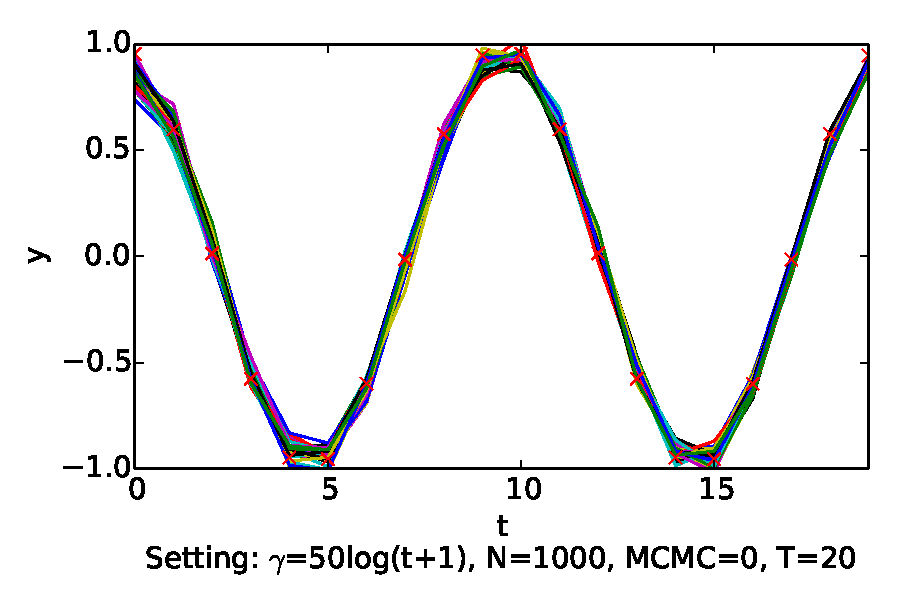
\includegraphics[width=\textwidth]{output_y/output_20_50log(t+1).pdf}
    \end{minipage}
    \begin{minipage}{0.5\textwidth}
        \centering
        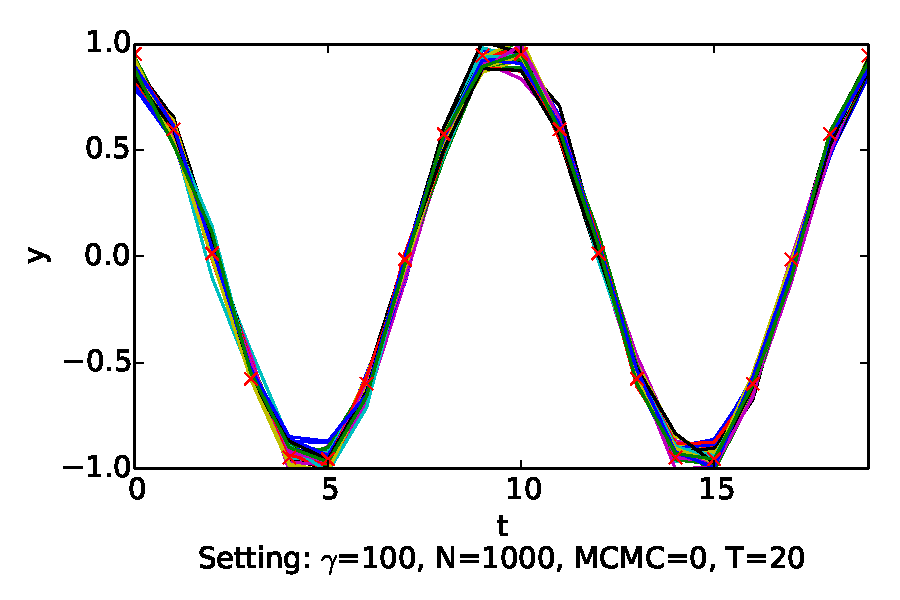
\includegraphics[width=\textwidth]{output_y/output_20_100.pdf}
    \end{minipage}%
    \begin{minipage}{0.5\textwidth}
        \centering
        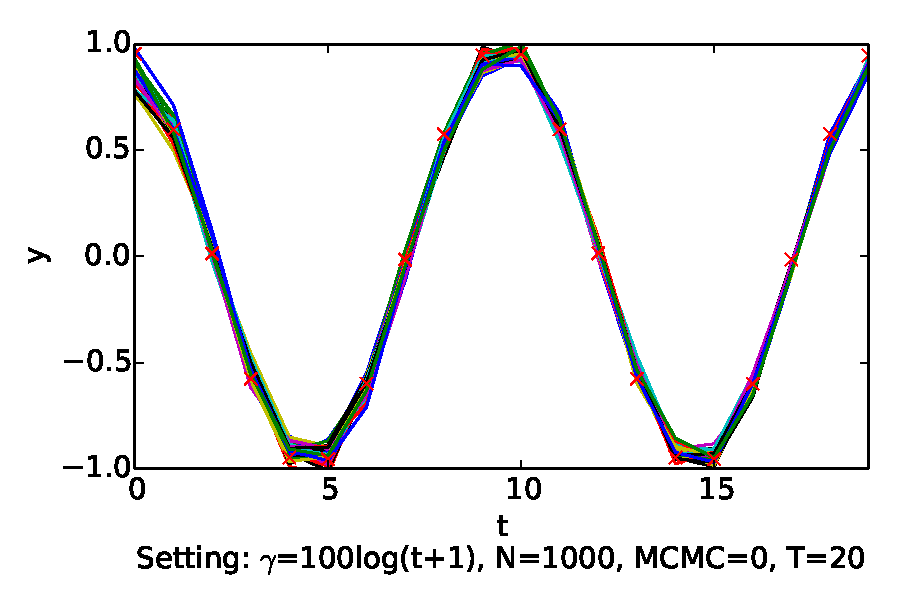
\includegraphics[width=\textwidth]{output_y/output_20_100log(t+1).pdf}
    \end{minipage}
    \begin{minipage}{0.5\textwidth}
        \centering
        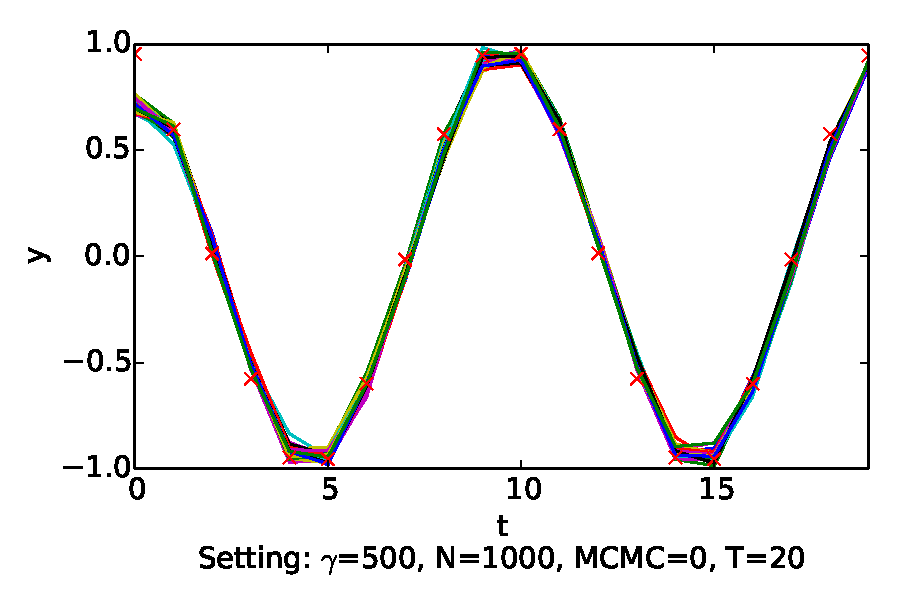
\includegraphics[width=\textwidth]{output_y/output_20_500.pdf}
    \end{minipage}%
    \begin{minipage}{0.5\textwidth}
        \centering
        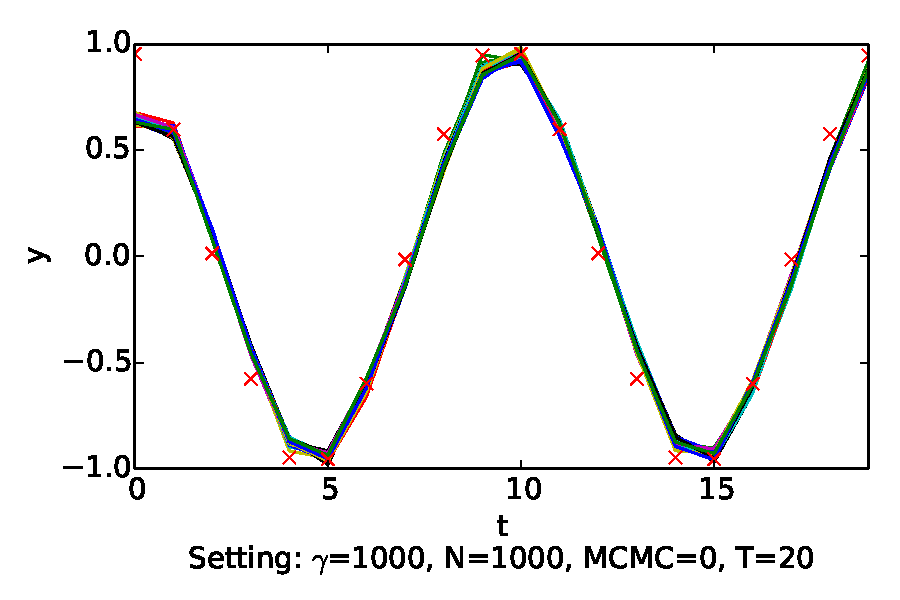
\includegraphics[width=\textwidth]{output_y/output_20_1000.pdf}
    \end{minipage}
    \caption{The means of the recursive likelihood $m_{t \mid t-1}(u^*_{1:T})$ obtained in $30$ independent runs with $T=20$, $N=1000$, various $\gamma$ settings and Resample-Move step disabled are plotted in lines with different colours. The target reference signal $y^{ref}$ is also plotted with a `x' marker.}
    \label{fig:estimatedy}
\end{figure}

\begin{figure}[!thbp]
    \centering
    \begin{minipage}{.5\textwidth}
        \centering
        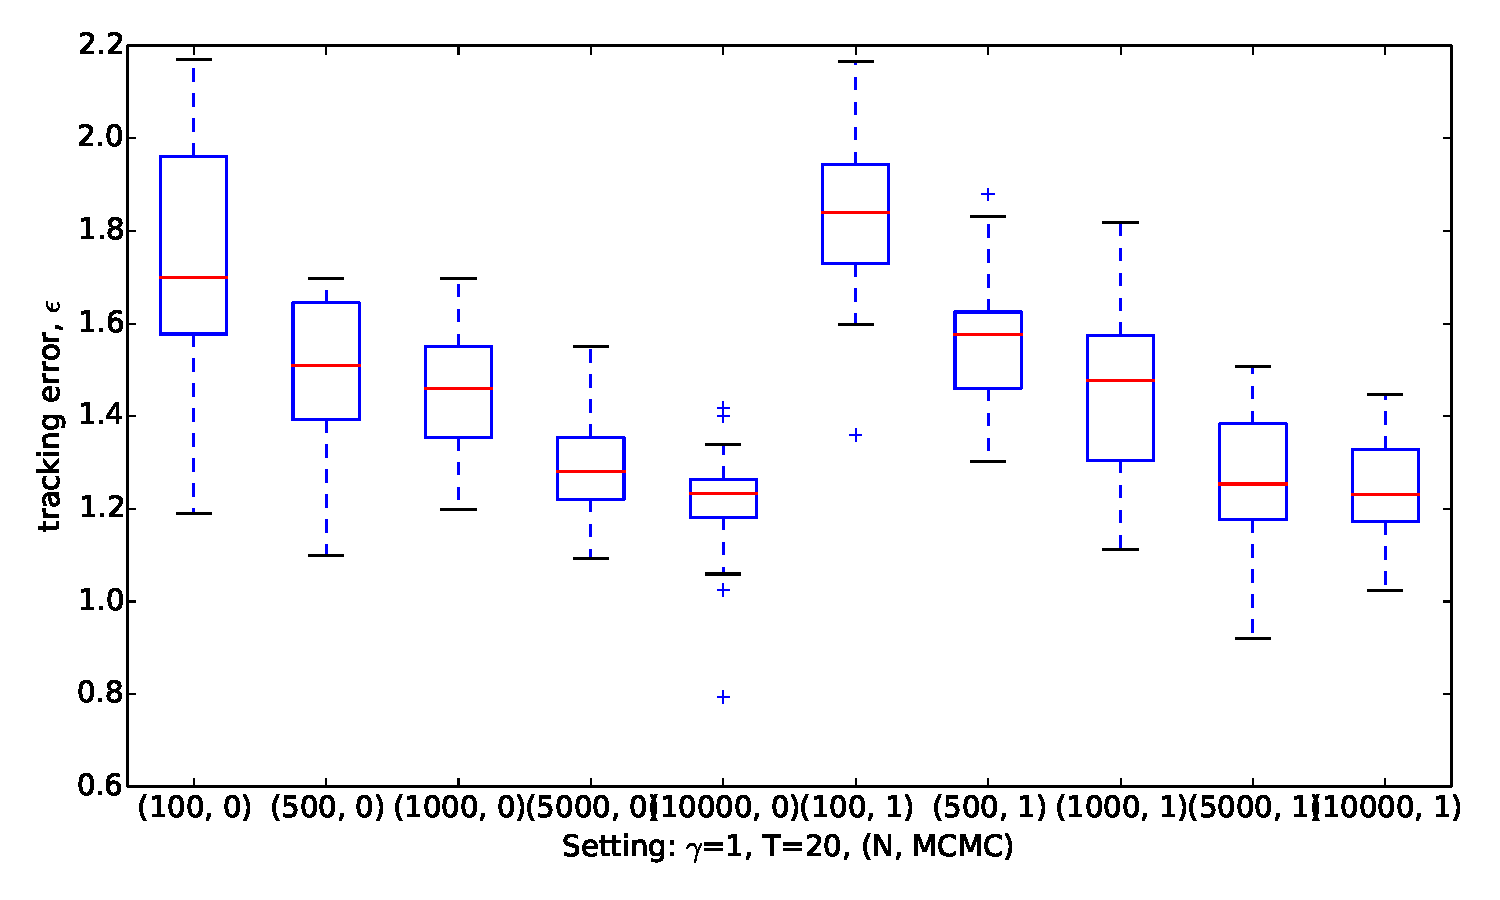
\includegraphics[width=\textwidth]{loglik_t_gs_n_error/T20_gamma1.pdf}
    \end{minipage}%
    \begin{minipage}{0.5\textwidth}
        \centering
        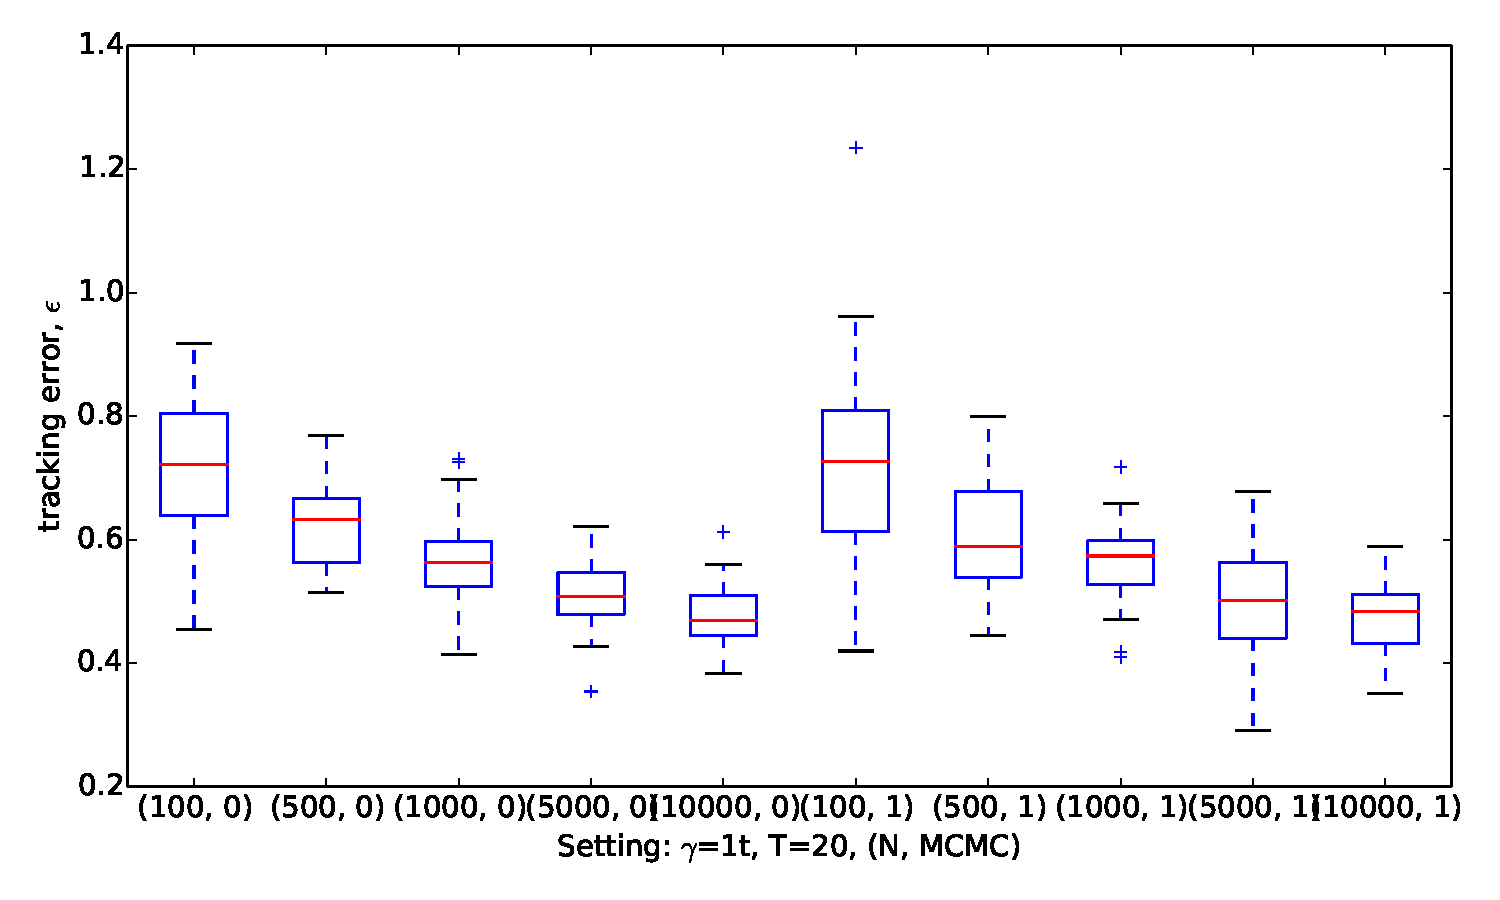
\includegraphics[width=\textwidth]{loglik_t_gs_n_error/T20_gamma1t.pdf}
    \end{minipage}
    \begin{minipage}{0.5\textwidth}
        \centering
        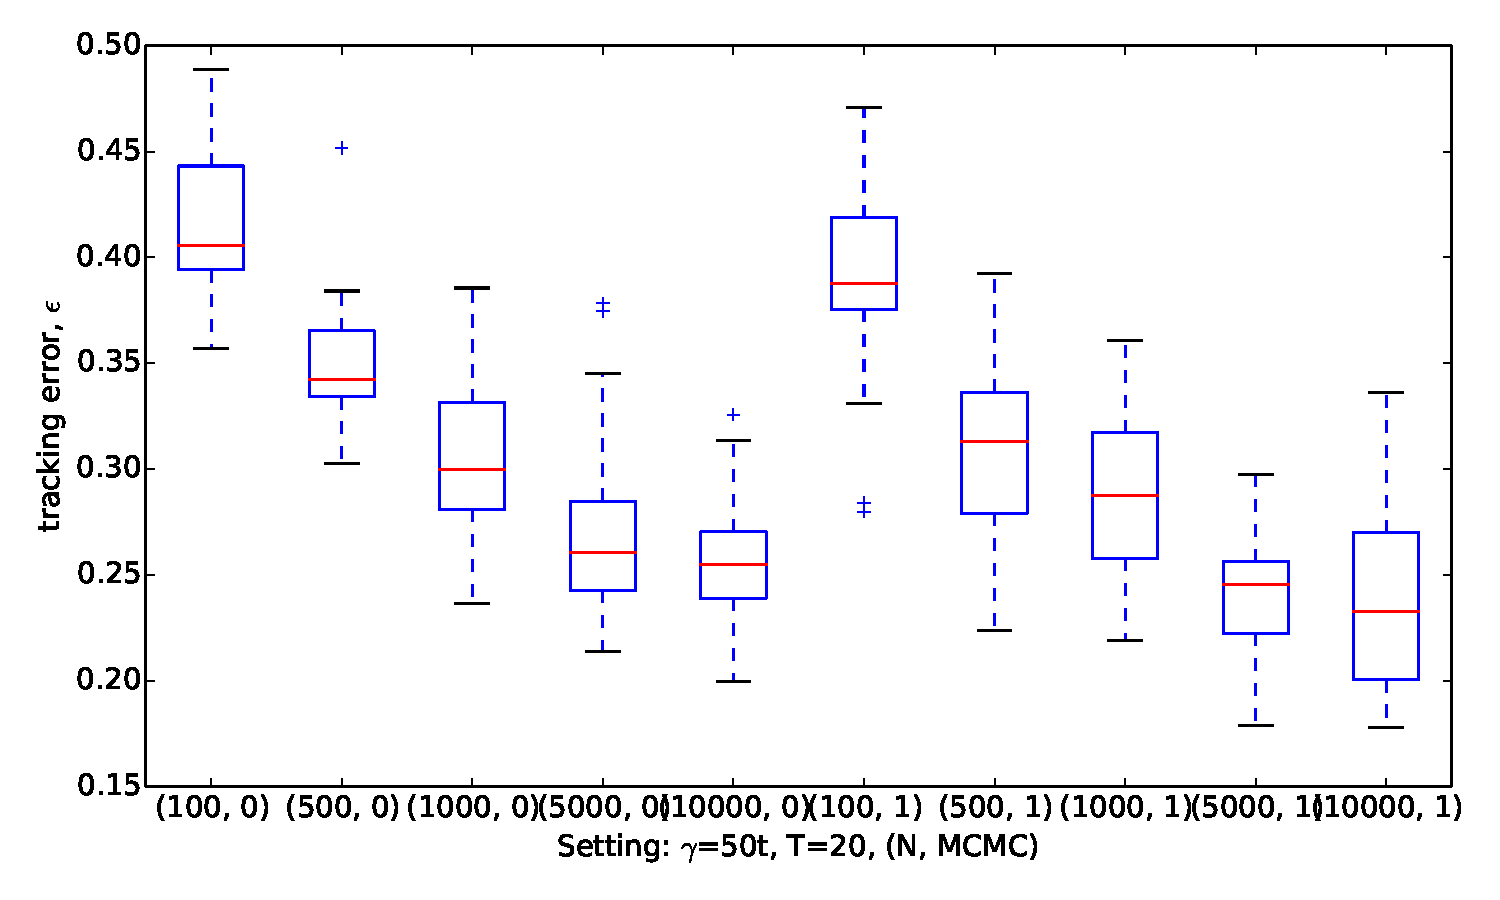
\includegraphics[width=\textwidth]{loglik_t_gs_n_error/T20_gamma50t.pdf}
    \end{minipage}%
    \begin{minipage}{0.5\textwidth}
        \centering
        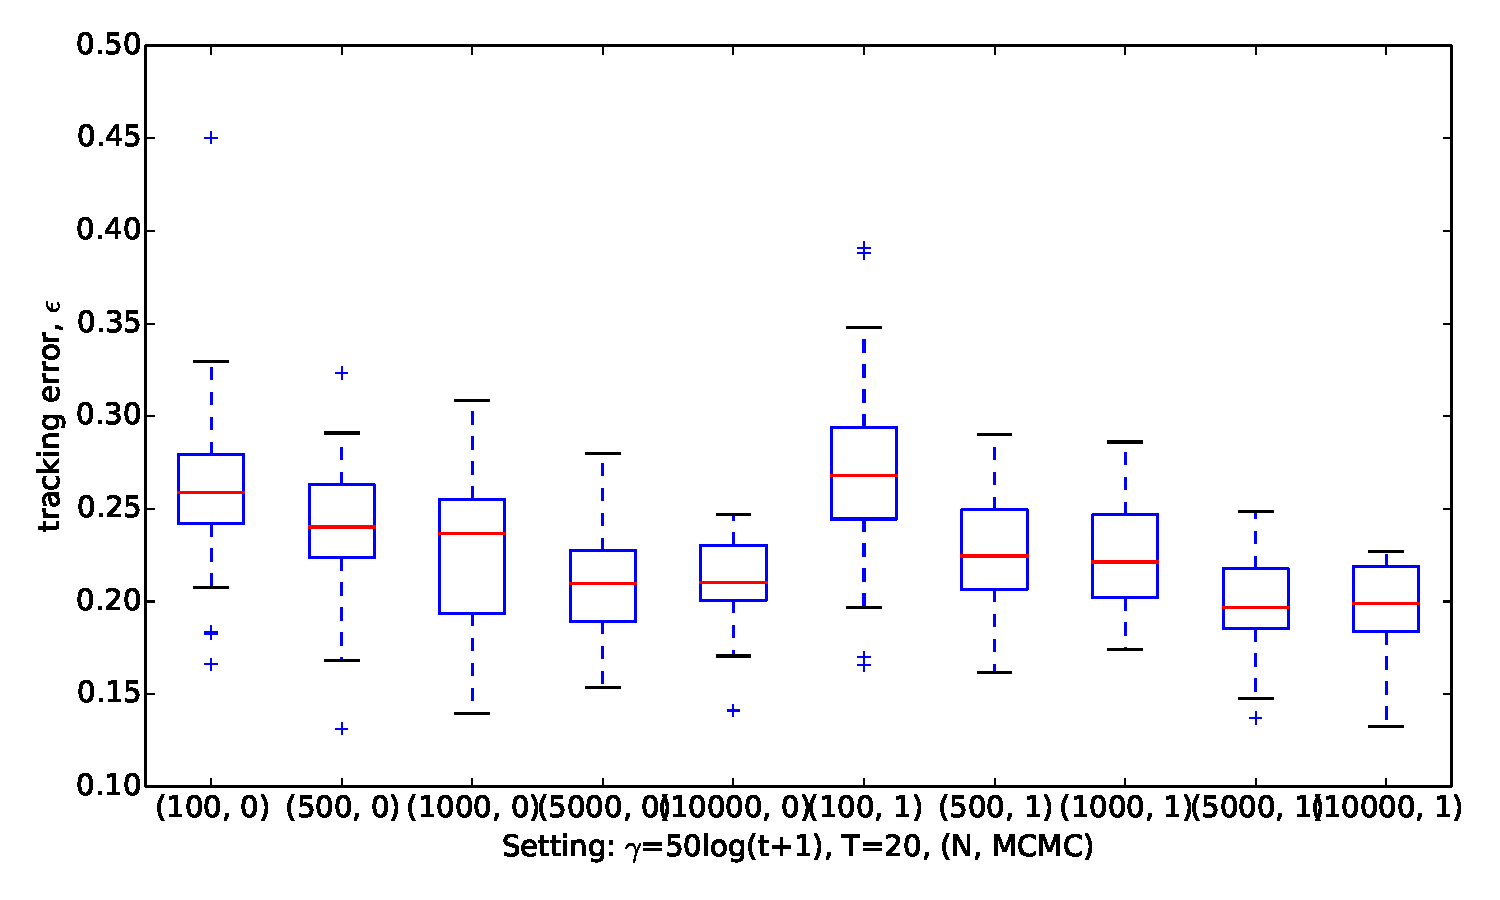
\includegraphics[width=\textwidth]{loglik_t_gs_n_error/T20_gamma50log(t+1).pdf}
    \end{minipage}
    \begin{minipage}{0.5\textwidth}
        \centering
        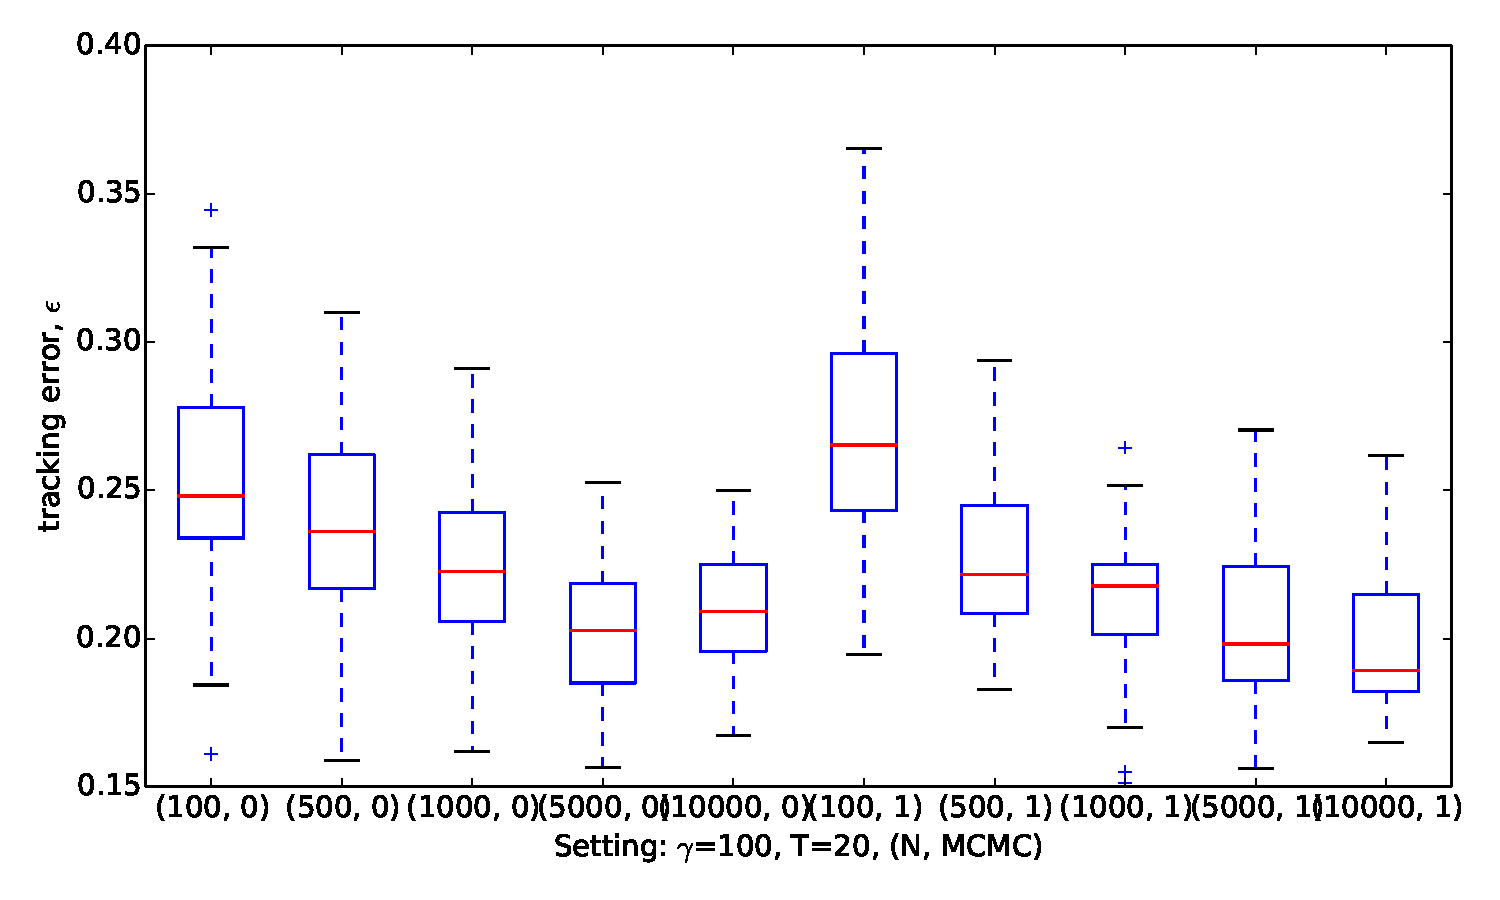
\includegraphics[width=\textwidth]{loglik_t_gs_n_error/T20_gamma100.pdf}
    \end{minipage}%
    \begin{minipage}{0.5\textwidth}
        \centering
        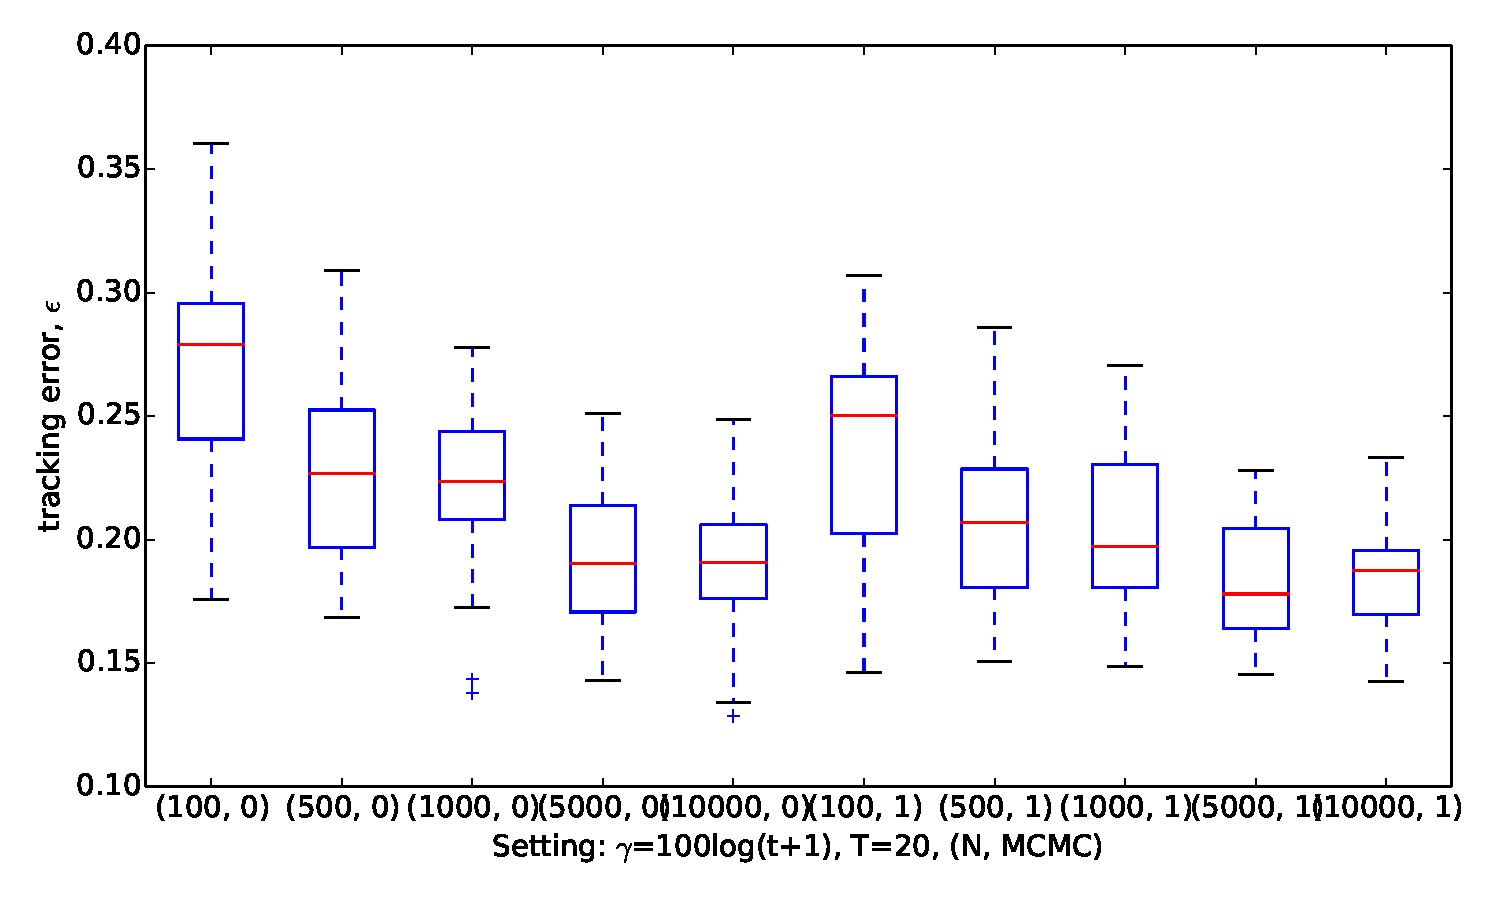
\includegraphics[width=\textwidth]{loglik_t_gs_n_error/T20_gamma100log(t+1).pdf}
    \end{minipage}
    \begin{minipage}{0.5\textwidth}
        \centering
        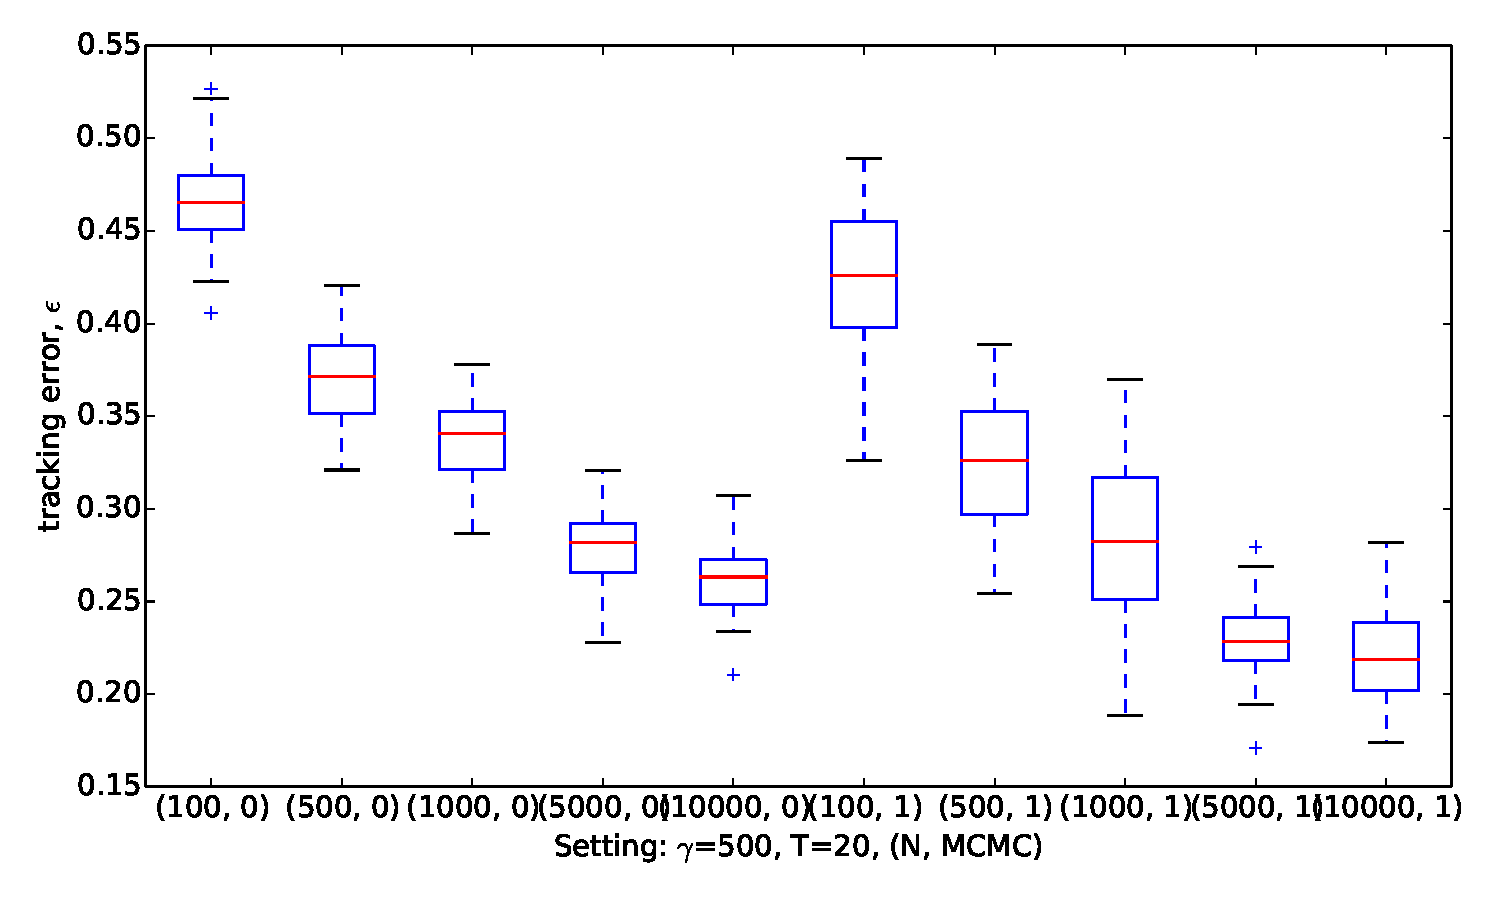
\includegraphics[width=\textwidth]{loglik_t_gs_n_error/T20_gamma500.pdf}
    \end{minipage}%
    \begin{minipage}{0.5\textwidth}
        \centering
        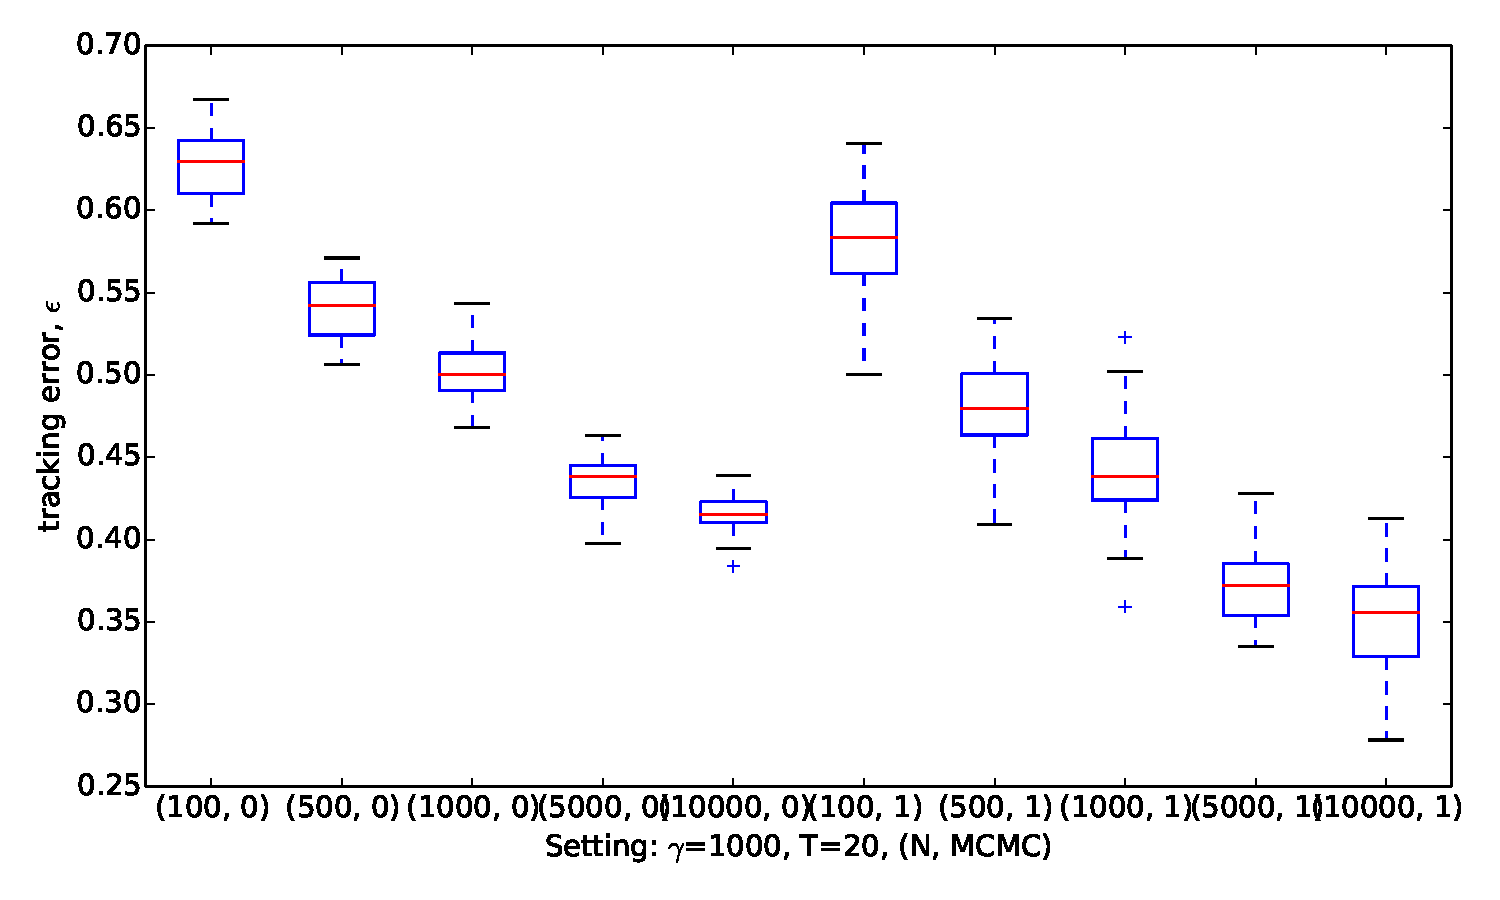
\includegraphics[width=\textwidth]{loglik_t_gs_n_error/T20_gamma1000.pdf}
    \end{minipage}
    \caption{The box-plots of tracking errors of the model using $u^*_{1:T}$ obtained in $30$ independent runs with $T=20$, $N=1000$, various $\gamma$ settings and Resample-Move step disabled.}
    \label{fig:error}
\end{figure}

\section{Conclusions}
In this chapter, we introduces the index tracking fund and summarise some causing factors of the tracking error between the fund and its benchmark index. We then present how the portfolio optimisation problem in terms of minimising the tracking error can be formulated as a stochastic control problem. This stochastic control problem can be turned into a path-space parameter estimation problem, in which Rao-Blackwellised SMC can be used to estimate these parameters efficiently. Lastly, we presents a some proof-of-concept experiment with a oscillating wave as target reference signal. The results show that the algorithm is able to track the reference signal well.

\chapter{Tracking the DAX index}
\graphicspath{{Chapter4/figures/}}
\label{cha:dax}
In this chapter, we attempt to use the same algorithm to a real-world financial index. We look at the German's DAX (Deutscher Aktienindex) Index, which consists of 30 German's blue chip stocks listed on Frankfurt Stock Exchange as the constituents from 1st January 2014 up to 30th June 2014. It represents $80\%$ of the aggregated prime standard's market capitalisation. The DAX Index is chosen for various pragmatic reasons. It is one of the major world indices that is tracked by various index funds, it has small number of components and the data is freely accessible\footnote{Actually, we first looked at Dow Jones Industrial Average (DJIA) Index obtained. It was later found some of the data is not publicly available. Having said that, the preliminary findings concur with the findings we have with the DAX Index reported here.}. For further detail on the DAX Index methodology, refer \cite{DAX14}.
 
\section{Tracking the DAX4 sub-index}
In the first experiment, we define a simple hypothetical sub-index, DAX4 consists of four stocks from the DAX Index that have the highest weights as of 2nd January 2014, namely Bayer (BAYN), Siemens (SIE), BASF (BAS) and Daimler (DAI). Then, the DAX4 index level is calculated as the simple weighted average of the adjusted close prices obtained from Yahoo Finance as follows:
\begin{equation}
  y^{DAX4} = \sum_{s \in \mathcal{S}} w_s x_s
\end{equation}
where $y^{DAX4}$ is the index level, $\mathcal{S}$ consists of the four stocks and  $w_s$ and $x_s$ are the weight and price of stock $s$ respectively. Here the weights of these four stocks are assigned to be $0.4$, $0.3$, $0.2$ and $0.1$ respectively. The adjusted close price of each stock along with the calculated index level are shown in Figure \ref{fig:adjclose}.
 
\begin{figure}[!thbp]
\centering
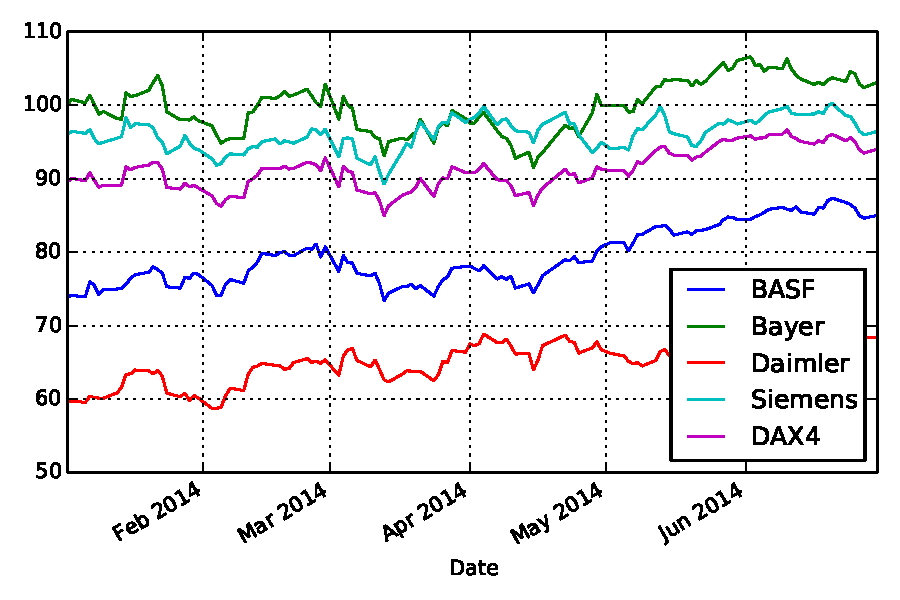
\includegraphics[width=\textwidth]{adjclose}
\caption{The adjusted close price of the 4 stocks and the calculated DAX4 index level, $y^{DAX4}$.}
\label{fig:adjclose}
\end{figure}
 
The portfolio optimisation problem is formulated as such $y^{DAX4}$ is viewed as the target reference level that a portfolio manager attempt to replicate as close as possible by changing the holding position on each component stocks in $\mathcal{S}$, at the same time, minimise the transaction cost incurred in position changes.
 
To solve this problem using the SMC,  the following state space modelling is used:
\begin{align}
  X_t &= X_{t-1} + F_t(U_t) + W_t \\
  Y_t &= U^T_tX_t + 0.01V_t
\end{align}
where $W_t \sim \mathcal{N}(\mu_{t_0}, \Sigma_{t_0})$, $V_t \sim \mathcal{N}(0, I)$, $\{X_t\}_{t \geq 0}$ is a vector of stock price processes modelled as Arithmetic Brownian Motion with drift, $\{U_t\}_{t \geq 0}$ is a vector of control input processes, each represents the position we have for each stock, $F_t(U_t)$ can be viewed as the market impact on price due to position changes and is set to be $0.0001U_t$ here, $\mu_{t_0}$ and $\Sigma_{t_0}$ are vector of the estimated mean returns and the estimated covariance matrix of the stock returns and $\{Y_t\}_{t \geq 0}$ is the process represents the index level.

The values of $\mu_t$ and $\Sigma_t$ here are estimated using Exponential Weighted Moving Average (EWMA) approach with the decay rate, $\lambda$, set to $0.94$. For example, $\mu_t$ can be easily calculated in a recursion form as follows:
\begin{equation}
  \mu_t = \lambda \mu_{t-1} + (1-\lambda) r_{t}
\end{equation}
where $r_t$ is the return at time step $t$. It is obvious from these equations that the EWMA estimate at time $t$ depends on all the preceding estimates at time $s$, where $s < t$. To ensure the quality of EWMA estimate, a 6 months warm up period is used, i.e., the EWMA estimate is calculated from 1st July 2013 onwards. The estimates of $\mu_{t_0}$ and $\Sigma_{t_0}$ obtained are as follows:
\begin{equation}
\mu_{t_0} =
\begin{blockarray}{c}
\\
\begin{block}{(c)}
~ 0.03125069 \\
0.20020445 \\
0.08702132 \\
0.18319923 \\
\end{block}
\end{blockarray}
~\Sigma_{t_0} =
\begin{blockarray}{ccccc}
  BAYN & SIE & BAS & DAI & \\
\begin{block}{(cccc)c}
 ~ 0.60011676 & 0.69688309 & 0.44198994 & 0.66709016 ~ & BAYN \\
0.69688309 & 1.34168488 & 0.58394515 & 0.76533660 & SIE \\
0.44198994 & 0.58394515 & 0.48855826 & 0.56500417 & BAS \\
0.66709016 & 0.76533660 & 0.56500417 & 1.13794411 & DAI \\
\end{block}
\end{blockarray}
\end{equation}
 
It is worth here to re-iterate here that this model is just a means to an end to demonstrate the idea. Other sophisticated models, e.g., Geometric Brownian Motion with drift, Jump diffusion model, etc., are possible, perhaps better.

Using this model, we can write the reward function as follows:
\begin{equation}
  J(u_{1:T},y^{ref}_{1:T}, x_0) = \E_{x_0}\left[ \exp \left( -\dfrac{1}{2}\displaystyle\sum^T_{t=1}\left(\vert\vert y^{ref}_t - u^Tx_t \vert\vert^2_{Q_t(u_t)^{-1}}  + \vert\vert u_t - u_{t-1} \vert\vert^2_{L_t}\right) \right ) \right]
\end{equation}
Here, we define $L = 0.1\diag(4,3,2,1)$  and also impose additional constraints on the holding position of each individual component of $U_t$ such that the range is within $[0,0.5]$. The idea behind these choices is to construct a scenario in which there is different amount of transaction cost involved in changing the holding position on each individual component and a constraint on the maximum amount on the holding position of each individual component one portfolio can have.

For simplicity, we will use the SMC algorithm to target $\pi$ directly, i.e, fixed $\gamma=100$ setting and important sampling step, $U_{1,n}$ is sampled uniformly from the range bounded the constraints mentioned. The experiment is carried out for $30$ independent runs, each with sample size is fixed to $10000$ and no Resample-Move step is used here.

\subsubsection{Results and discussion}
As in previous experiment, the estimated optimal control $u^*_{1:T}$ and the mean of the recursive likelihood $m_{t \mid t-1}(u^*_{1:T})$ obtained in one of the independent runs are shown in Figure \ref{fig:dax}.  It is obvious the output of the model produce using the estimated $\hat{u}^*_{1:T}$ is closely tracking the reference index level, $y^{DAX4}$. The average annualised\footnote{the annualisation factor is set to be $\sqrt{252}$ as the daily return is measured here.} tracking error of $0.023288$ over the $30$ runs. Having said that, the estimated set of control parameter $\hat{u}^*_{1:T}$ which represents the holding position of each stock does not seem very stable.

\begin{figure}[tbp]
\centering
    \begin{minipage}{0.5\textwidth}
        \centering
        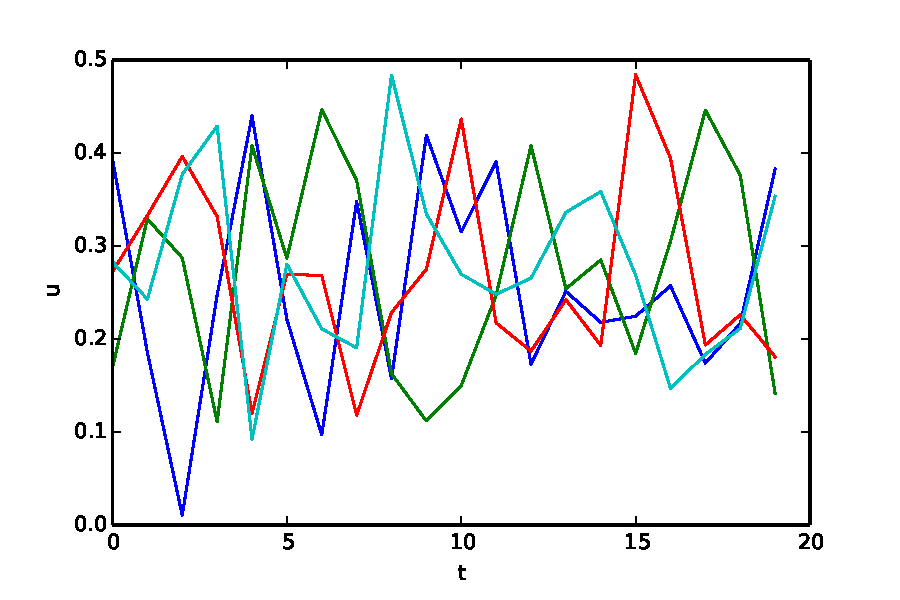
\includegraphics[width=\textwidth]{DAX4Low-u.pdf}
    \end{minipage}%
    \begin{minipage}{0.5\textwidth}
        \centering
        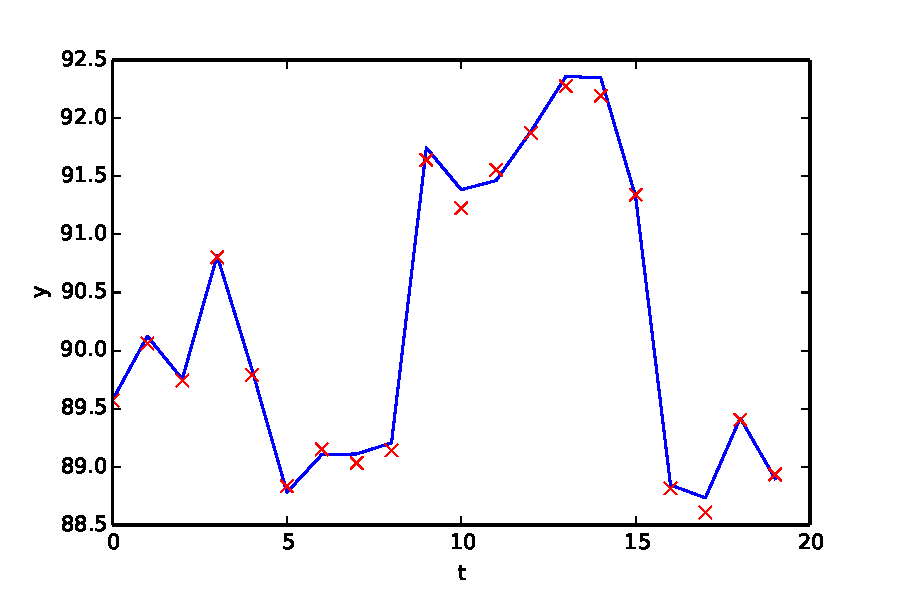
\includegraphics[width=\textwidth]{DAX4Low-y.pdf}
    \end{minipage}
\caption{The estimated optimal control $u^*_{1:T}$ and the mean of the recursive likelihood $m_{t \mid t-1}(u^*_{1:T})$ obtained in one of the independent runs with the $y^{DAX4}$ set to be the target reference using $L = 0.1\diag(4,3,2,1)$.}
\label{fig:dax4}
\end{figure}

To reduce the number of changes in holding positions, the value of $L$ matrix can be scaled up. To demonstrate this, the same experiment is re-run with $L = 5\diag(4,3,2,1)$. The results are shown in Figure \ref{fig:dax42}. It is obvious the estimated set of control parameters $\hat{u}^*_{!:T}$ produced in this case is much more stable. However, this comes at a price on the tracking error. The average annualised tracking error with this setting is increased to $0.036386$ over the $30$ runs. 

\begin{figure}[htbp]
\centering
    \begin{minipage}{0.5\textwidth}
        \centering
        \includegraphics[width=\textwidth]{DAX4High-u.pdf}
    \end{minipage}%
    \begin{minipage}{0.5\textwidth}
        \centering
        \includegraphics[width=\textwidth]{DAX4High-y.pdf}
    \end{minipage}
\caption{The estimated optimal control $u^*_{1:T}$ and the mean of the recursive likelihood $m_{t \mid t-1}(u^*_{1:T})$ obtained in one of the independent runs with the $y^{DAX4}$ set to be the target reference using $L = 5\diag(4,3,2,1)$.}
\label{fig:dax42}
\end{figure}

\subsection{Tracking the DAX index}
Given the results of the experiment for DAX4 index look promising, we now attempt to track the original DAX index which consists of $30$ components using a similar model as follows:
\begin{align}
  X_t &= X_{t-1} + F_t(U_t) + W_t \\
  Y_t &= 30U^T_tX_t + 0.01V_t
\end{align}
where $W_t \sim \mathcal{N}(\mu_{t_0}, \Sigma_{t_0})$, $V_t \sim \mathcal{N}(0, I)$, along with the same parameter settings as before except the following:
\begin{enumerate}
\item The target reference $y^{ref}$ is the daily close level of the DAX index level.
\item The number of dimensions for $U_t$ and $X_t$ are now $30$.
\item The $L$ matrix is set to be $5I_{30 \times 30}$, where $I_{n \times n}$ is the $n$ dimensional identity matrix, i.e., the transaction cost of each component is equal.
\end{enumerate}

As mentioned in Section \ref{sec:replication}, sometimes it can be more efficient not only just in terms of computational, but also in terms of transaction cost and management perspective to track the benchmark index with only a subset of its component stocks. To do this, only minimal changes are required to apply on the model proposed. We choose to use the top $6$ highest weighted constituents of DAX index by including Allianz SE ($ALV$) and SAP SE ($SAP$), in which they all together constitute more than $50\%$ of the weights for the DAX index level as of 2nd January 2014. Using only these $6$ component stocks and a slight increase on the range of each component of $U_t$ to within $[0,1]$, the experiment is re-run for $30$ times.

\subsubsection{Results and discussion}
As before, the estimated optimal control $u^*_{1:T}$ and the mean of the recursive likelihood $m_{t \mid t-1}(u^*_{1:T})$ obtained in one of the independent runs with the DAX index level set to be the target reference for both the full replication setting and partial replication setting are shown in Figure \ref{fig:dax} and \ref{fig:daxpartial} respectively.

In the full replication setting, the average annualised tracking error over $30$ runs is found to be $0.113118$. However, the computational cost increases significantly in this experiment due to the dimensionality increases in $U$ and $X$. Using the computation cost of the previous $DAX4$ experiment as the baseline, the computational cost for this experiment is $\approx 7.2$ times more per time step.

In the partial replication setting, the average annualised tracking error over $30$ runs is found to be $0.062650$. The estimated optimal control $u^*_{1:T}$ found in this setting is also much stable. This means smaller changes in holding positions and therefore lesser transaction costs. In terms of computational cost, the relative computational cost factor in comparison to the baseline is approximately $1.1$. This translates to approximately $6.5\times$ speed-up in comparison to the full replication setting.

\begin{figure}[htbp]
\centering
    \begin{minipage}{0.5\textwidth}
        \centering
        \includegraphics[width=\textwidth]{DAXFull-u.pdf}
    \end{minipage}%
    \begin{minipage}{0.5\textwidth}
        \centering
        \includegraphics[width=\textwidth]{DAXFull-y.pdf}
    \end{minipage}
\caption{The estimated optimal control $u^*_{1:T}$ and the mean of the recursive likelihood $m_{t \mid t-1}(u^*_{1:T})$ obtained in one of the independent runs with the DAX index level set to be the target reference using all $30$ component stocks.}
\label{fig:dax}
\end{figure}

\begin{figure}[htbp]
\centering
    \begin{minipage}{0.5\textwidth}
        \centering
        \includegraphics[width=\textwidth]{DAXPartial-u.pdf}
    \end{minipage}%
    \begin{minipage}{0.5\textwidth}
        \centering
        \includegraphics[width=\textwidth]{DAXPartial-y.pdf}
    \end{minipage}
\caption{The estimated optimal control $u^*_{1:T}$ and the mean of the recursive likelihood $m_{t \mid t-1}(u^*_{1:T})$ obtained in one of the independent runs with the DAX index level set to be the target reference using only the $6$ component stocks with highest weights.}
\label{fig:daxpartial}
\end{figure}

\section{Model Predictive Control (MPC)}
Up to this point, the discussion has been focussed on predicting the optimal (as outlined in the reward function) strategy for the a given time period $0:T$. However, as time progress, more realisation of the reference signal $y^{ref}_{t^\prime}, t^\prime < T$ are observed. It makes sense to take this information into account in the optimisation process. In this section, we shall demonstrate how the SMC technique can be integrated into Model Predictive Control (MPC) framework.

MPC is an established technique in control theory which has achieved significant success in many different domains. It is a kind of receding horizon control algorithm, in which at time step $t$, the model is used to optimise the controls for the process, $u_{t:t+K}$ for a finite horizon for $t:t+K$. However, only the first set of controls, i.e., $u_{t}$ is applied to the system. At time $t+1$, the new set of the observation is measured to update the states. Then, the whole optimisation process is repeated for the same horizon, but shifted by one time step until $t=T$. The MPC framework is summarised in Algorithm \ref{algo:mpc}. Refer \cite{RJB09,MJM02} for further details on MPC. 

\begin{algorithm}
\caption{Model Predictive Control}\label{algo:mpc}
\begin{algorithmic}[1]
\Function{ModelPredictiveControl}{T,K}
\State Set $t \gets 1$.
\While{$t \leq T$}
\State Search the optimal $u^*_{t:t+K}$ for the control problem of time horizon $t:t+K$.
\State Apply the first set of the optimal control  $u^*_{t}$ to the problem.
\State Update the model states with any new measurement $y^{ref}_t$.
\State Set $t \gets t + 1$.
\EndWhile
\EndFunction
\end{algorithmic}
\end{algorithm}

To use MPC framework here, the SMC based optimisation algorithm can be executed on a daily basis after the market close on day $t$ to search for the optimal $u^*_{t:t+K}$, but only apply the first set of controls, $u_t$ to the problem. The same algorithm is repeated on the next day with a shifted time horizon and so on. Using this model, the reward function that we attempt to optimise at each time step $t$ is as follows:
\begin{equation}
  J(u_{t:t+K},y^{ref}_{t:t+K}, x_t) = \E_{x_0}\left[ \exp \left( -\dfrac{1}{2}\displaystyle\sum^{t+K}_{s=t}\left(\vert\vert y^{ref}_s - u^Tx_s \vert\vert^2_{Q_s(u_s)^{-1}}  + \vert\vert u_s - u_{s-1} \vert\vert^2_{L_s}\right) \right ) \right]
\label{eq:J2}
\end{equation}

To demonstrate this idea, we re-run the DAX index with partial replication setting using this MPC framework with $K=5$. The experiment is repeated for $30$ times. The results look very promising. Figure \ref{fig:mpc} shows the estimated optimal control $u^*_{1:T}$ and the mean of the recursive likelihood $m_{t \mid t-1}(u^*_{1:T})$ obtained in one of the independent runs. The tracking performance looks good, with an average annualised tracking error of $0.062813$ over the $30$ runs. The estimated optimal control $u^*_{1:T}$ found is also reasonable stable. In terms of computational cost, the relative computational cost factor in comparison to the baseline is approximately $5.5$ for each time step.
 
\begin{figure}[htbp]
\centering
    \begin{minipage}{0.5\textwidth}
        \centering
        \includegraphics[width=\textwidth]{DAXMPC-u}
    \end{minipage}%
    \begin{minipage}{0.5\textwidth}
        \centering
        \includegraphics[width=\textwidth]{DAXMPC-y}
    \end{minipage}
\caption{The estimated optimal control $u^*_{1:T}$ and the mean of the recursive likelihood $m_{t \mid t-1}(u^*_{1:T})$ obtained in one of the independent runs with the DAX index level set to be the target reference using the MPC framework with $K=5$.}
\label{fig:mpc}
\end{figure}

In practice, the target reference signal $y^{ref}_{t+1:t+K}$ would not be observable at time step $t$. To over this, we define an estimator of $y^{ref}$ to be as follows:
\begin{equation}
  \hat{y}^{ref}_{t+k} = y^{ref}_{t} + \beta k
\end{equation}
where $k$ is within $1 \ldots K$, $\beta$ is the EWMA estimate ($\lambda = 0.94$) of the daily changes of $y^{ref}$ up to time step $t$. This estimator is chosen here for simplicity. Other estimators are possible.

Using the estimate $\hat{y}^{ref}_{t+1:t+K}$ in place of $y^{ref}_{t+1:t+K}$, the reward function $J$ defined in \eqref{eq:J2} now only depends information up to time step $t$. With this setting, the experiment is re-run for $30$ times. Figure \ref{fig:mpc2} shows the estimated optimal control $u^*_{1:T}$ and the mean of the recursive likelihood $m_{t \mid t-1}(u^*_{1:T})$ obtained in one of the independent runs. The tracking performance looks good, with an average annualised tracking error of $0.062364$ over the $30$ runs. The estimated optimal control $u^*_{1:T}$ found is also reasonable stable.

\begin{figure}[htbp]
\centering
    \begin{minipage}{0.5\textwidth}
        \centering
        \includegraphics[width=\textwidth]{DAXMPC-u-2}
    \end{minipage}%
    \begin{minipage}{0.5\textwidth}
        \centering
        \includegraphics[width=\textwidth]{DAXMPC-y-2}
    \end{minipage}
\caption{The estimated optimal control $u^*_{1:T}$ and the mean of the recursive likelihood $m_{t \mid t-1}(u^*_{1:T})$ obtained in one of the independent runs with the estimated DAX index level ($\hat{y}^{ref}_{t:t+K}$) set to be the target reference using the MPC framework with $K=5$.}
\label{fig:mpc2}
\end{figure}

\section{Conclusions}
\label{sec:conclusion5}
This chapter presents several experiments in apply the SMC technique to track a real-world financial index --- the DAX index.  It begins with a simple experiment in which a synthetic sub-index constructed with only $4$ to proof the concept. It then uses the same technique to demonstrate how the DAX index can be tracked with full replication as well as partial replication. Lastly, it introduces Model Predictive Control (MPC) framework and demonstrates how this technique can be integrated into the MPC framework easily. In all cases, the results sow the SMC technique proposed is able to search for optimal control that results an output that track the reference signal given.

\chapter{Conclusions and future work}
\graphicspath{{Chapter5/figures/}}
\label{cha:conclusions}
The work reported in the previous chapter provides evidence to support
the thesis hypothesis:
\begin{quote}
Sequential Monte Carlo (SMC) techniques have the potential to be an effective means of searching the optimal strategy for index tracking funds.
\end{quote}
This chapter reviews the work that has been done, evaluates the extent
to which they justify the thesis hypothesis and concludes the thesis
by addressing the directions for future work.

\section{Contributions}
In the first experiment, we demonstrated the potential of SMC techniques in tracking a deterministic simple oscillating wave. The sensitivity of the techniques in terms of parameter settings and trade-off between the estimation accuracy and computational efforts are explored numerically. Several results are found. Firstly, it is found that a simple resampling step at each iteration performs better the more advanced method in which the resampling step is selectively triggered depending on the ESS value. Secondly, it is found that the improvement of resample-move step is marginal. Considering the amount of computational cost involved and the extra amount of design cost involved, this may not be worthwhile. Thirdly, it is found that setting $\gamma$ as an increasing function of $t$ does lead to better performance, albeit extra care must be paid on the amount of increment at each step to avoid pre-mature convergence to local optimal. 

In the second experiment, we explore the potential of SMC techniques in searching the optimal strategy for index tracking error with constraints and minimizing the transaction costs. We adopt the same framework with slightly different model. Although this framework has been applied in various engineering domains, there is no previous work to my knowledge in the application of such techniques in portfolio tracking error optimisation. In particular, we show how index can be fully replicated or partially replicated with transaction cost taken into account. The experiment results show the SMC techniques are rather promising.

In the third experiment, we introduce the concept of model predictive control (MPC) and how it can be used together with SMC techniques in improving tracking performance. Whist this technique is nothing new in control theory, its application to this portfolio optimisation problem is novel. The experimental results do suggest that MPC indeed improve the tracking performance.

\section{Envisaged future work}
Having discussed the contributions of the thesis, we now outline
numerous possible directions for future work that have been identified
during the course of this research.

\subsection{More realistic models}
The Arithmetic Brownian Model with drift used in this thesis is rather simple. A possible extension work is to consider a more advanced model, e.g., Geometric Brownian Model, Jump Diffusion model, etc. Moving away from conditional Gaussian model also introduces another complication. Without the conditional Gaussian assumption, the inner Kalman Filter recursion is no longer optimal. A possible solution to this is substituting the Kalman Filter with a nested SMC algorithm. This setup is known as the SMC2 algorithm \cite{CN13}.

\subsection{Parallel computation}
The nested SMC setup inevitably add consideration computation requirements. A possible speed up is to parallelise the steps in SMC algorithm. This is very straight-forward for all the steps, except the resampling step, which remains an interesting research topic on its own. 

\subsection{More complex financial indices}
The benchmark index used in this thesis is rather simple. This can
be potentially an issue. Having said that, this index is a simple, but by no means a ``toy''
index. It is a major financial index in the world. There are however indices with much large number of components, e.g., $\approx 1600$ for MSCI World Index. This translates to a high dimensional problem in which may be difficult for the proposed model here.

A possible way to cope with this is to just track the index with partial replication using preselected subset of components, perhaps using Principle Component Analysis (PCA). Alternatively, we could use a divide and conquer approach, tracking multiple sub-indices separately. Yet, there is still much to answer here, for example:
\begin{itemize}
\item How to split an index into smaller components in a systematic manner?
\item How to deal with index components changes during announcement and implementation?
\end{itemize}

\section{Closing remarks}
\label{ClosingRemark}
The work reported in this thesis demonstrates a considerable degree of
originality supported by extensive experimentation. The case studies
are necessarily limited given the limited amount of time frame.  However, the results
 demonstrate that portfolio optimisation using Sequential Monte Carlo techniques have very considerable promise. We recommend these approaches to
the research community for further investigation.


%%% ----------------------------------------------------------------------

% ------------------------------------------------------------------------

%%% Local Variables: 
%%% mode: latex

%%% TeX-master: "../thesis"
%%% End: 

\appendix
\chapter{Kalman Filter}
\graphicspath{{Appendices/figures/}}
\label{sec:KF}
In a conditional linear Gaussian state space as follows:
\begin{align}
  X^L_t &= A_t(X^N_t)X^L_{t-1} + B_t(X^N_t)W_t + F_t(X^N_t) \\
  Y_t &= C_t(X^N_t)X^L_t + D_t(X^N_t)V_t + G_t(X^N_t)
\end{align}
where $\{X^N_t\}_{t \geq 0}$ is a non-linear Markov process, $A_t$, $B_t$, $C_t$, $D_t$, $F_t$, $G_t$ are appropriate matrix/vector of $X^N_t$ and  $\{W_t\}_{t \geq 0}$ and  $\{V_t\}_{t \geq 0}$ are independent sequences of standard Gaussian random variables, i.e., $W_t, V_t \sim \mathcal{N}(0,I)$. In such a case, the transition density and likelihood of this model are Gaussian distributions with centre lied at a point of a linear combination of the known $x^N_t$ of the following form:
\begin{align}
  f_t(x^L_t \mid x^L_{t-1}, x^N_t) &= \mathcal{N}(A_t(x^N_t) x^L_{t-1} + F_t(x^N_t), B_t(x^N_t)B_t(x^N_t)^T) \nonumber \\
  g_t(y^L_t \mid x^L_t, x^N_t)    &= \mathcal{N}(C_t(x^N_t) x^L_t + G_t(x^N_t), D_t(x^N_t)D_t(x^N_t)^T)
\end{align}

Using the properties of Gaussian distribution, the integral involved can be resolved analytically. This leads to the widely used \emph{Kalman Filter} \cite{KRE60} that has the following recursive solution as follows:
\begin{align}
  \mu_{t \mid t -1} &= A_{t}(x^N_t)(\mu_{t-1 \mid t-1})X_{t-1} + F_t(x^N_t) \\
  \Sigma_{t \mid t -1} &= A_{t}(x^N_t)\Sigma_{t -1 \mid t -1}A_{t}(x^N_t)^T +  B_t(x^N_t)B_t(x^N_t)^T \\
  S_t &=  C_{t}(x^N_t)\Sigma_{t \mid t -1}C_{t}(x^N_t)^T +  D_t(x^N_t)D_t(x^N_t)^T \\
  m_{t \mid t-1} &=  C_{t}(x^N_t)  \mu_{t \mid t-1} + G_t(x^N_t) \\
  \mu_{t \mid t} &=   \mu_{t \mid t-1} +   \Sigma_{t \mid t -1} C_{t}(x^N_t)S_t^{-1}(y_t - m_{t \mid t-1}) \\
  \Sigma_{t \mid t} &=  \Sigma_{t \mid t -1} -\Sigma_{t \mid t -1} C_{t}(x^N_t)S_t^{-1} C_{t}(x^N_t)\Sigma_{t \mid t -1}
\end{align}
where  $\mu_{t \mid t -1}$ and $\Sigma_{t \mid t-1}$ are the predicted mean and co-variance matrix of the state $x^L_t$, $m_{t \mid t-1}$ and $S_t$ are the mean and co-variance matrix of the measurement at time $t$ and $\mu_{t \mid t}$ and $\Sigma_{t \mid t}$ are the estimated mean and co-variance matrix of the state $x^L_t$ after seeing the observation $y_t$.

There are various extensions have been developed on top of this approach. For example, the Extended Kalman Filter (EKF) which uses Taylor Series expansion to linearise at the conditional variables locally \cite{WG95}, Unscented Kalman Filter which further extend the idea in EKF by only using a minimal set of well chosen samples \cite{EW01}, etc.

\endinput
%%% ----------------------------------------------------------------------

% ------------------------------------------------------------------------

%%% Local Variables: 
%%% mode: latex

%%% TeX-master: "../thesis"
%%% End: 

%\bibliographystyle{Classes/CUEDbiblio}
%\bibliographystyle{Classes/jmb}
\addcontentsline{toc}{chapter}{References} %adds References to contents page
\bibliographystyle{acm} %this works with package natbib
%\bibliographystyle{Classes/jmb} % bibliography style
\renewcommand{\bibname}{References} % changes default name Bibliography to References
\bibliography{References/references} % References file



\end{document}
